\documentclass[mscthesis]{usiinfthesis}
\usepackage{lipsum}
\usepackage{listings}
\usepackage{pstricks}
\usepackage{auto-pst-pdf}
\usepackage{array}
\usepackage{color}
\usepackage{colortbl}
\usepackage{multirow}
\usepackage[nomain,acronym,toc]{glossaries}

\makeglossaries
\newacronym{simd}{SIMD}{Single Instruction, Multiple Data Streams}
\newacronym{sisd}{SIMD}{Single Instruction, Single Data Stream}
\newacronym{hsmm}{HSMM}{Hidden Semi-Markov Model}
\newacronym{hmm}{HMM}{Hidden Markov Model}
\newacronym{gpu}{GPU}{Graphics Processing Unit}
\newacronym{cpu}{CPU}{Central Processing Unit}
\newacronym{gpp}{GPP}{General Purpose Processor}
\newacronym{asic}{ASIC}{Application Specific integrated Circuit}
\newacronym{fpga}{FPGA}{Field Programmable Gate Array}
\newacronym{dsp}{DSP}{Digital Signal Processor}
\newacronym{dspv}{DSP}{Digital Signal Processing}
\newacronym{hpcs}{HPCS}{High Productivity Computing Systems}
\newacronym{blas}{BLAS}{Basic Linear Algebra Subroutines}
\newacronym{svm}{SVM}{Support Vector Machine}
\newacronym{smo}{SMO}{Sequential Minimal Optimization}
\newacronym{sw}{SW}{Software}
\newacronym{hw}{HW}{Hardware}
\newacronym{rtl}{RTL}{Register Transfer Level}
\newacronym{lzc}{LZC}{Leading Zero Counter}
\newacronym{fifo}{FIFO}{First In, First Out}
\newacronym{macc}{MACC}{Multiply-Accumulate}
\newacronym{cdf}{CDF}{Cumulative Distribution Funtion}
\newacronym{ram}{RAM}{Random Access Memory}
\newacronym{rom}{ROM}{Read Only Memory}
\newacronym{csr}{CSR}{Compressed Sparse Row}
\newacronym{coo}{COO}{Coordiante}
\newacronym{ell}{ELL}{ELLPACK/ITPACK}
\newacronym{bv}{BV}{Bit-Vector}
\newacronym{cbv}{CBV}{Compressed Bit-Vector}
\newacronym{cvbv}{CVBV}{Compressedi Variable-Length Bit-Vector}
\newacronym{dft}{DFT}{Dispersion Frame Technique}
\newacronym{svd}{SVD}{Singular Value Decomposition}


% customizations
\definecolor{mygreen}{rgb}{0,0.4,0}
\definecolor{mygray}{rgb}{0.5,0.5,0.5}
\definecolor{mymauve}{rgb}{0.58,0,0.82}
\definecolor{mysmokegray}{rgb}{0.9,0.9,0.9}

\lstset{
    backgroundcolor=\color{mysmokegray},
    basicstyle=\footnotesize\ttfamily,
    breaklines=true,
    captionpos=b,
    commentstyle=\itshape\color{mygreen},
    escapeinside={//*}{\^^M},
    keywordstyle=\bfseries\color{blue},
    linewidth=0.95\linewidth,
    mathescape=true,
    numbers=left,
    numberstyle=\tiny\color{mygray},
}

\DeclareMathOperator{\erf}{erf}
\lstdefinelanguage{algebra}
{morekeywords={import,sort,constructors,observers,transformers,axioms,if,
else,end},
sensitive=false,
morecomment=[l]{//s},
}

%===============================================================================
%%%%%%%%%%%%%%%%%%%%%%%%%%%%%%%%%%%%%%%%%%%%%%%%%%%%%%%%%%%%%%%%%%%%%%%%%%%%%%%%
\title{Accelerator for Event-based Failure Prediction} %compulsory
\specialization{Embedded Systems Design}%optional
\subtitle{Acceleration of an Extended Forward Algorithm for Failure Prediction
    on \acrshort{fpga}}
\author{Simon Maurer} %compulsory
\begin{committee}
    \advisor{Prof.}{Miroslaw}{Malek} %compulsory
    %\coadvisor{Prof.}{Student's}{Co-Advisor}{} %optional
\end{committee}
\Day{29.} %compulsory
\Month{Janaury} %compulsory
\Year{2014} %compulsory, put only the year
\place{Lugano} %compulsory

%\dedication{To my beloved} %optional
%\openepigraph{Someone said \dots}{Someone} %optional

%\makeindex %optional, also comment out \theindex at the end

\begin{document}

\maketitle %generates the titlepage, this is FIXED

\frontmatter %generates the frontmatter, this is FIXED

\begin{abstract}
\end{abstract}

%\begin{abstract}[Zusammenfassung]
%optional, use only if your external advisor requires it in his/er
%language 
%\\
%
%\lipsum
%\end{abstract}

\begin{acknowledgements}
\end{acknowledgements}

\tableofcontents 
\listoffigures %optional
\listoftables %optional
\lstlistoflistings

\mainmatter

%===============================================================================
%%%%%%%%%%%%%%%%%%%%%%%%%%%%%%%%%%%%%%%%%%%%%%%%%%%%%%%%%%%%%%%%%%%%%%%%%%%%%%%%
\chapter{Introduction}
\label{ch:intro}
\glsresetall % reset acronyms

In today's live it becomes increasingly important, that computer systems are
dependable. The reason being, that computer systems are used more and more in
areas where the failure of such a system can lead to catastrophic events.
Banking, public transportation and medical engineering are only a few examples
of areas employing large and extremely complex systems. The increasing
complexity of computer systems has a direct impact on their maintainability and
testability. It is simply impossible to guarantee that a piece of \gls{sw} comes
without any faults. On top of that, the same problematic arises with the
\gls{hw} components which also may contain faulty parts but also get
increasingly prone to failures due to decay of material.

In the event of a system failure it is of course desirable to fix the system as
soon as possible in order to minimize the downtime of the system (maximize the
availability). This can be accomplished by using different types of recovery
techniques, e.g. check-pointing (create checkpoints to roll back/forward), fail
over (switch to a redundant system), reboot. All these techniques require
a certain amount of time to complete the recovery process, time that is very
valuable. In order to minimize this time, techniques have been developed to
anticipate upcoming failures. Such a technique is described in
\cite{salfner08}, which will be the reference work for this thesis.

The work \cite{salfner08} presents an algorithm to predict failures and
compares the results with other techniques. The accuracy of the presented
algorithm to predict failures proves to be better compared to the other
techniques, has however the drawback of increased complexity and hence
increased computation time. It is very important to keep the computation
overhead very low in order to maximize the time between the prediction of
a failure and the actual event of the failure. One way to decrease the
computation time is to design a \gls{hw} accelerator for the prediction
algorithm. The design of such an accelerator is outlined in this document.

%-------------------------------------------------------------------------------
%===============================================================================
\section{Problem Statement}
\label{ch:_intro_prob}

The main idea of the prediction model proposed in the reference work
\cite{salfner08} is to predict failures, based on sequences of events and their
time of arrival. This is modeled with a \gls{hsmm}. A very detailed description
can be found in the reference work, but the fundamental concept is also
described here, in chapter \ref{ch:event}. In order to perform a prediction,
three parts are required: the training of the model, the sequence processing
and the classification. The training of the model uses collected error event
data samples and corresponding oracle predictions (collected from known
failures) to train the features (parameters) of the model in order to be able
to detect similar sequences as the ones that led to failures in previous cases.
The training of the model is not time critical and is performed off-line. The
trained features are then used in the second part, the sequence processing.
This is now time critical as this happens on-line on a live system. The system
will continuously send error events to the sequence processing unit, which
needs to compute a likelihood of the sequence of the last $L$ events. This
likelihood is sent to a classifier where it is compared to a non-failure
likelihood. The classifier then predicts if the sequence at hand will lead to
a failure in the near future.

The failure prediction method, as it was outlined in very few words above and
discussed in \cite{salfner08}, leads to very good prediction results (F-measure
of up to 0.66. See chapter \ref{ch:event} for more information). This comes at
the price of high computational efforts that are necessary to perform the
sequence processing. This may lead to the situation that a failure is correctly
predicted, but the result of the prediction is only available after the failure
has already happened. This would of course rend the prediction useless. The
main goal of this thesis, aims to accelerate the sequence processing part in
order to predict a failure before it really happens. To do so, first available
parallelism and an appropriate accelerator architecture must be found. Then the
accelerator must be designed and implemented, using the knowledge gained from
the analysis and finally the implementation must be compared to a serial
implementation and a speedup and accuracy must be computed.

%-------------------------------------------------------------------------------
%===============================================================================
\section{Motivation}
\label{ch:intro_mot}

As already outlined before, it becomes increasingly important to provide
dependable infrastructure for information systems. Failure prediction is a very
hot research topic with a main focus on server infrastructure. With the recent
trend of moving everything to the cloud, one may question the usefulness of
failure prediction of single nodes. Rather than focusing on single machines it
may prove beneficial to focus on the interaction of nodes and predict failures
on a bigger scale. Why then designing a accelerator for a prediction model that
targets single server systems?

Despite the trend of moving to the cloud, there are still thousands of single
node systems that have a huge impact on a vast amount of people and failures
would prove to be catastrophic. The talk is about embedded systems. Embedded
systems are everywhere and the number is increasing. While server farms are
growing, there is also the trend of specializing information systems. With the
advances of computer \gls{hw}, performance is available with less space and
energy requirements and hence machines are getting more intelligent with the
increasing trend to embed powerful systems. Transportation (trains, planes,
cars) is a prime example of dependable embedded systems. Huge efforts have been
made to make fully autonomous transportation systems failure prone (e.g. bullet
train in Japan) by adding redundant recourses. Accurate failure prediction
systems may be a key to reduce these recourses or to increase the
dependability.

Another issue with the proposed failure prediction method is the high amount of
parameters that need to be identified, estimated and set. Even if this initial
work is done, the process must be repeated after some time interval, due to the
fact that properties of server system change during their lifetime. This is
usually not the case for embedded systems. Once an embedded system is designed
and installed, \gls{sw} changes are a lot less common (neglecting the consumer
market which is not the main target here), hence the system parameters do not
change often or not at all. It is therefore sufficient to do the parameter
configuration only once during design time. Another aspect is the specific
application domain of embedded systems. They are designed for very specific
functions and offer a better insight in process properties than this is the
case with complex \gls{sw} architectures on server systems. A parametrization
of the failure prediction system for an embedded system, will in general prove
to be easier than for server systems.

These are the reason why this work presents an acceleration for the failure
prediction method proposed by \cite{salfner08}. The accelerator will be designed
with special attention on low resource and energy requirements, as the main
targets are single node embedded systems for industrial applications.

%-------------------------------------------------------------------------------
%===============================================================================
\section{Structure}
\label{ch:intro_struct}

This section gives an overview of the structure of the thesis. Chapter
\ref{ch:art} presents existing work, done in the aria of failure prediction and
acceleration of related algorithms. Chapter \ref{ch:event} provides a short
summary of the prediction model to be accelerated and presents the results
obtained by using the prediction model in a real case scenario. This is
discussed in detail in the reference work \cite{salfner08}. Chapter
\ref{ch:analysis} focuses on the sequence prediction algorithm and provides an
analysis of available parallelism. In chapter \ref{ch:design} a design of an
accelerator is proposed and in chapter \ref{ch:results} results in terms of
speedup and accuracy are presented.  Chapter \ref{ch:conc} concludes the work
by presenting the contributions and outlines possible future work related to
the acceleration.

%===============================================================================
%%%%%%%%%%%%%%%%%%%%%%%%%%%%%%%%%%%%%%%%%%%%%%%%%%%%%%%%%%%%%%%%%%%%%%%%%%%%%%%%
\chapter{State of the Art}
\label{ch:art}
\glsresetall % reset acronyms

This section provides an overview of the state of the art in the different
fields of research that are relevant for the thesis. This includes failure
prediction methods, existing solutions to accelerate failure prediction
algorithms and acceleration techniques in general.

%-------------------------------------------------------------------------------
%===============================================================================
\section{Failure Prediction}
\label{ch:art_pred}
A very detailed overview of failure prediction methods is given in
\cite{ACM10_Salfner}. The survey discusses i.a. the techniques used as
comparison in the main reference
\cite{lin88,IEEE90_lin,ICDM02_Vilalta,domeniconi02} as well as the technique
described in the main reference \cite{salfner08}.

More recent work uses \gls{hw} counters of a general purpose \gls{cpu} and
combines them with \gls{sw} instrumentation to analyze failures of single
processes (e.g grep, flex, sed) \cite{FSE10_Yilmaz}. As industry heads more and
more towards cloud computing, it has been proposed to use information of
interaction between nodes (instead of analyzing single nodes) in order to
analyze and predict failures of a distributed system
\cite{IEEE12_Salfner,DSN10_Oliner}.

%-------------------------------------------------------------------------------
%===============================================================================
\section{Accelerator}
\label{ch:art_acc}

The main goal of this master thesis is to accelerate an adaptation of the
forward algorithm. Proposals for a \gls{gpu} based accelerator for the classic
forward algorithm are described in \cite{neumann11,liu09}. Further, several
proposals to accelerate the Viterbi algorithm (which is closely related to the
forward algorithm) have been published: \cite{ASAP12_Azhar} presents an
architecture for a lightweight Viterbi accelerator designed for an embedded
processor datapath, \cite{IPDPS07_Jacob,ICS06_Maddimsetty,IPDPS07_Oliver}
describe a \gls{fpga} based accelerator for protein sequence \gls{hmm} search
and \cite{IPDPS09_Walters} describes i.a. an approach to accelerate the Viterbi
algorithm from the HMMER library\footnote{http://hmmer.janelia.org/} using
\glspl{gpu}.

Focusing on a more general approach for acceleration, \cite{ARITH13_Kadric}
proposes an \gls{fpga} implementation of a parallel floating point accumulation
and \cite{ITNG07_Yang} describes the implementation of a vector processor on
\gls{fpga}.

Quite some research has been done on the question what type of technology
should be used to accelerate certain algorithms: \cite{SASP08_Che} presents
a performance study of different applications accelerated on a multicore
\gls{cpu}, on a \gls{gpu} and on a \gls{fpga}, \cite{FPL10_Jones} discusses the
suitability of \gls{fpga} and \gls{gpu} acceleration for \gls{hpcs} without
focusing on a specific application and \cite{ISVLSI10_Kestur} also focuses on
\gls{hpcs} but uses the \gls{blas} as comparison and also takes \glspl{cpu}
into account.

It may be interesting to also think about an acceleration of the model
training. Similar work has been done by accelerating \glspl{svm}:
\cite{FCCM09_Cadambi} describes a \gls{fpga} based accelerator for the
\gls{svm}-\gls{smo} algorithm used in the domain of machine learning and
\cite{IEEE03_Anguita} proposes a new algorithm and its implementation on
a \gls{fpga} for \glspl{svm}.

%===============================================================================
%%%%%%%%%%%%%%%%%%%%%%%%%%%%%%%%%%%%%%%%%%%%%%%%%%%%%%%%%%%%%%%%%%%%%%%%%%%%%%%%
\chapter{Event-based Failure Prediction}
\label{ch:event}
\glsresetall % reset acronyms

This section provides a brief overview of the computational steps done by the
proposed algorithm described in the reference work \cite{salfner08}.

To be able to understand the formal expression of the algorithm, first
a definition of the used parameters is provided.
\begin{itemize}
    \item N: number of states of the \gls{hsmm}
    \item M: number of observation symbols (size of the alphabet)
    \item L: observation sequence length
    \item R: number of \gls{cdf} (kernels)
\end{itemize}
The delay of the event at time $ t_k $ with respect to the event at time
$ t_{k-1} $ is described as
\begin{equation}
\label{eq:delay}
    d_k = t_k-t_{k-1}
\end{equation}

The proposed failure prediction method aims to find sequences of error events
that led to failures in the system on previous occasions. Additional to
a specific sequence of events, also the time of arrival of the event is taken
into account (or more precise, the delay as defined in equation
\ref{eq:delay}). The error events that are produced by the system usually need
to be preprocessed or brought in to a form understandable for the predictor.
The error events must build a set of distinct symbols, denoted as $A=\{o_1,
\dots, o_M\}$. This set is also called alphabet of size $M$. Details on
preprocessing the events can be found in section \ref{ch:event_data}.

To detect specific sequences of events by also taking the time of arrival into
account, an extension of the \gls{hmm} is proposed. The resulting model is
called \acrfull{hsmm}. A extended forward algorithm is used to compute
a likelihood, which is then used in a classifier to decide if a failure is
predicted. Section \ref{ch:event_sequ} presents the formal definitions of the
algorithm on how the sequences are processed and section \ref{ch:event_class}
describes the classification.

In order to predict failure types with sequence processing, the \gls{hsmm} has
to be trained. The training is performed with an adaptation of the Baum-Welch
algorithm. Section \ref{ch:event_train} provides a very brief description and
lists the trained features necessary for the sequence processing.

The system supports multiple failure types, where for each type a separate
model must be built. Additionally a non-failure model is built in order to
classify sequences. Figure \ref{fig:model} provides a schematic overview of
a complete prediction model with multiple failure types.

\begin{figure}
    \centering
    % Generated with LaTeXDraw 2.0.8
% Sat Jun 28 18:45:28 CEST 2014
% \usepackage[usenames,dvipsnames]{pstricks}
% \usepackage{epsfig}
% \usepackage{pst-grad} % For gradients
% \usepackage{pst-plot} % For axes
\scalebox{1} % Change this value to rescale the drawing.
{
\begin{pspicture}(0,-5.8421874)(9.62,5.8121877)
\definecolor{color1152b}{rgb}{0.7843137254901961,0.7843137254901961,1.0}
\pspolygon[linewidth=0.02,fillstyle=solid,fillcolor=color1152b](1.61,5.8021874)(7.21,5.8021874)(7.21,3.8021874)(4.61,3.8021874)(4.61,3.2021875)(4.81,3.2021875)(4.41,2.6021874)(4.01,3.2021875)(4.21,3.2021875)(4.21,3.8021874)(1.61,3.8021874)
\pspolygon[linewidth=0.02,fillstyle=solid,fillcolor=color1152b](0.01,0.6021875)(2.81,0.6021875)(2.81,-0.1978125)(1.61,-0.1978125)(1.61,-0.7978125)(1.81,-0.7978125)(1.41,-1.3978125)(1.01,-0.7978125)(1.21,-0.7978125)(1.21,-0.1978125)(0.01,-0.1978125)
\pspolygon[linewidth=0.02,fillstyle=solid,fillcolor=color1152b](3.01,0.6021875)(5.81,0.6021875)(5.81,-0.1978125)(4.61,-0.1978125)(4.61,-0.7978125)(4.81,-0.7978125)(4.41,-1.3978125)(4.01,-0.7978125)(4.21,-0.7978125)(4.21,-0.1978125)(3.01,-0.1978125)
\pspolygon[linewidth=0.02,fillstyle=solid,fillcolor=color1152b](6.81,0.6021875)(9.61,0.6021875)(9.61,-0.1978125)(8.41,-0.1978125)(8.41,-0.7978125)(8.61,-0.7978125)(8.21,-1.3978125)(7.81,-0.7978125)(8.01,-0.7978125)(8.01,-0.1978125)(6.81,-0.1978125)
\pspolygon[linewidth=0.02,fillstyle=solid,fillcolor=color1152b](0.01,-1.3978125)(2.81,-1.3978125)(2.81,-2.1978126)(1.61,-2.1978126)(2.21,-2.7978125)(2.41,-2.5978124)(2.61,-3.3978126)(1.81,-3.1978126)(2.01,-2.9978125)(1.21,-2.1978126)(0.01,-2.1978126)
\pspolygon[linewidth=0.02,fillstyle=solid,fillcolor=color1152b](3.01,-1.3978125)(5.81,-1.3978125)(5.81,-2.1978126)(4.61,-2.1978126)(4.61,-2.7978125)(4.81,-2.7978125)(4.41,-3.3978126)(4.01,-2.7978125)(4.21,-2.7978125)(4.21,-2.1978126)(3.01,-2.1978126)
\pspolygon[linewidth=0.02,fillstyle=solid,fillcolor=color1152b](6.81,-1.3978125)(9.61,-1.3978125)(9.61,-2.1978126)(8.41,-2.1978126)(7.61,-2.9978125)(7.81,-3.1978126)(7.01,-3.3978126)(7.21,-2.5978124)(7.41,-2.7978125)(8.01,-2.1978126)(6.81,-2.1978126)
\pspolygon[linewidth=0.02,fillstyle=solid,fillcolor=color1152b](1.21,-3.3978126)(6.41,-3.3978126)(6.01,-4.1978126)(4.61,-4.1978126)(4.61,-4.7978125)(4.81,-4.7978125)(4.41,-5.3978124)(4.01,-4.7978125)(4.21,-4.7978125)(4.21,-4.1978126)(1.21,-4.1978126)
\pspolygon[linewidth=0.02,fillstyle=solid,fillcolor=color1152b](6.61,-3.3978126)(8.41,-3.3978126)(8.41,-4.1978126)(6.21,-4.1978126)
\psline[linewidth=0.04cm,arrowsize=0.05291667cm 2.0,arrowlength=1.4,arrowinset=0.4]{->}(2.21,4.4021873)(6.61,4.4021873)
\psline[linewidth=0.04cm](3.01,4.6021876)(3.01,4.2021875)
\psline[linewidth=0.04cm](4.41,4.6021876)(4.41,4.2021875)
\psline[linewidth=0.04cm](5.21,4.6021876)(5.21,4.2021875)
\usefont{T1}{ptm}{m}{n}
\rput(3.0171876,4.8071876){B}
\usefont{T1}{ptm}{m}{n}
\rput(4.4171877,4.8071876){C}
\usefont{T1}{ptm}{m}{n}
\rput(5.2365627,4.8071876){A}
\psframe[linewidth=0.04,linestyle=dashed,dash=0.16cm 0.16cm,framearc=0.5,dimen=outer](5.61,5.2021875)(2.61,4.0021877)
\usefont{T1}{ptm}{m}{n}
\rput(4.3909373,5.5021877){\footnotesize Observed Error Sequence}
\pspolygon[linewidth=0.02,fillstyle=solid,fillcolor=color1152b](0.01,2.6021874)(0.01,1.8021874)(1.21,1.8021874)(1.21,1.2021875)(1.01,1.2021875)(1.41,0.6021875)(1.81,1.2021875)(1.61,1.2021875)(1.61,1.8021874)(4.21,1.8021874)(4.21,1.2021875)(4.01,1.2021875)(4.41,0.6021875)(4.81,1.2021875)(4.61,1.2021875)(4.61,1.8021874)(6.01,1.8021874)(6.41,2.6021874)
\pspolygon[linewidth=0.02,fillstyle=solid,fillcolor=color1152b](6.61,2.6021874)(6.21,1.8021874)(8.01,1.8021874)(8.01,1.2021875)(7.81,1.2021875)(8.21,0.6021875)(8.61,1.2021875)(8.41,1.2021875)(8.41,1.8021874)(9.61,1.8021874)(9.61,2.6021874)
\psline[linewidth=0.06cm,linestyle=dotted,dotsep=0.16cm](6.01,0.2021875)(6.61,0.2021875)
\psline[linewidth=0.06cm,linestyle=dotted,dotsep=0.16cm](6.01,-1.7978125)(6.61,-1.7978125)
\usefont{T1}{ptm}{m}{n}
\rput(4.4035935,-3.7978125){\footnotesize Classification}
\usefont{T1}{ptm}{m}{n}
\rput(1.3865625,-1.5978125){\footnotesize Sequence}
\usefont{T1}{ptm}{m}{n}
\rput(1.3610938,-1.9978125){\footnotesize Likelihood 0}
\usefont{T1}{ptm}{m}{n}
\rput(4.3865623,-1.5978125){\footnotesize Sequence}
\usefont{T1}{ptm}{m}{n}
\rput(8.186563,-1.5978125){\footnotesize Sequence}
\usefont{T1}{ptm}{m}{n}
\rput(4.4471874,-1.9978125){\footnotesize Likelihood 1}
\usefont{T1}{ptm}{m}{n}
\rput(8.166562,-1.9978125){\footnotesize Likelihood u}
\usefont{T1}{ptm}{m}{n}
\rput(6.6585937,4.2071877){t}
\usefont{T1}{ptm}{m}{n}
\rput(4.4245315,2.2021875){\footnotesize Pre-processing}
\usefont{T1}{ptm}{m}{n}
\rput(1.389375,0.4021875){\footnotesize Sequence Recognition}
\usefont{T1}{ptm}{m}{n}
\rput(1.4217187,0.0021875){\footnotesize Model 0}
\usefont{T1}{ptm}{m}{n}
\rput(4.409375,0.4021875){\footnotesize Sequence Recognition}
\usefont{T1}{ptm}{m}{n}
\rput(8.209375,0.4221875){\footnotesize Sequence Recognition}
\usefont{T1}{ptm}{m}{n}
\rput(4.4078126,0.0021875){\footnotesize Model 1}
\usefont{T1}{ptm}{m}{n}
\rput(8.227187,0.0021875){\footnotesize Model u}
\usefont{T1}{ptm}{m}{n}
\rput(4.476719,-5.6978126){\footnotesize Failure Prediction}
\end{pspicture} 
}


    \caption{Overview of the failure prediction approach. Model 0 is trained
        with non-failure sequences}
    \label{fig:model}
\end{figure}

%-------------------------------------------------------------------------------
%===============================================================================
\section{Data Processing}
\label{ch:event_data}

The failure prediction method is based on error events. The most common form of
how error events are saved is log entries in a file structure. Although work
has been done to propose standardized techniques on how log events should be
stored (\cite{IPDPS04_Salfner, DSN09_Ziming}), it is still not very common to
follow such approaches. This results in a huge forest of different log
structures that makes automated processing of such data difficult. Common
issues that need to be taken care of are: different representation of time
stamps, numbers in log messages that need to be filtered (e.g. process id),
typos and different text messages with the same meaning.

The reference work \cite{salfner08} describes methods on how to process log
files and create unique error ids that then build an alphabet of symbols. This
has been done on real case data. In this work no \gls{hw} or \gls{sw} solution
is provided to pre-process data. It is assumed that the events are already in
a form that is readable by the accelerator.

%-------------------------------------------------------------------------------
%===============================================================================
\section{Training of the Model}
\label{ch:event_train}

The model training is based on an extension of the Baum-Welch Algorithm. This
part will not be accelerated due to its non-criticality with respect to time.
For this reason only a very brief description of the algorithm is presented.
For a much more detailed explanation and proof, refer to \cite{salfner08}.
The training is used to estimate the parameters for each \gls{hsmm}. Using
the term of machine learning, these parameters are called features.

The features to be trained are used by the extended forward algorithm, which is
used to calculate a sequence likelihood of a \gls{hsmm}. This is described in
the next section. Following the features:
\begin{itemize}
    \item $ \pi_i $, forming the initial state probability vector
        $ \boldsymbol{\pi} $ of size $ N $
    \item $ b_i(o_j) $, forming the emission probability matrix $ B $ of size
        $ N \times M $
    \item $ p_{ij} $, forming the matrix of limiting transmission probabilities
        $ P $ of size $ N \times N $
    \item $ \omega_{ij, r} $, the weights of the kernel $ r $
    \item $ \theta_{ij, r} $, the parameters of the kernel $ r $
\end{itemize}

The estimation of the features can be done by using real error event logs,
associated to real failures. The time and id of each error event as well as the
time and type of the failure are known. With an iterative approach (Baum-Welch
algorithm), the features can be estimated in order to allow the \gls{hsmm} to
produce a value that describes the likelihood of a specific event sequence to
produce a failure of a specific type. Due to the proposed extension of also
taking the delay of an event into account, the Baum-Welch algorithm was
extended with a gradient descent approach to estimate the kernel parameters.

%-------------------------------------------------------------------------------
%===============================================================================
\section{Sequence Processing}
\label{ch:event_sequ}

The following description will provide a complete blueprint of the extended
forward algorithm, without any explanations or proofs related to the
formulation. Those are provided in \cite{salfner08}. While the basic forward
algorithm is used to calculate a sequence likelihood of a \gls{hmm}, with the
extension it is possible to do the same for the proposed \gls{hsmm}. The
extension takes into account that events are not emitted with a constant period.
This variance of the delay (cf. \ref{eq:delay}) is modeled by introducing
one or more \glspl{cdf} also called kernels. The extended forward algorithm is
formally defined as follows:

\begin{equation}
    \label{eq:forward_init}
    \alpha_0(i) = \pi_{i}b_{s_i}(O_0) \\
\end{equation}
\begin{equation}
    \label{eq:forward}
    \alpha_k(j) = \sum_{i=1}^{N} \alpha_{k-1}(i) v_{ij}(d_k) b_{s_j}(O_k);
    \quad 1 \leq k \leq L
\end{equation}
where
\begin{equation}
    \label{eq:V}
    v_{ij}(d_k) = \left\{
        \begin{array}{l l}
            p_{ij} d_{ij}(d_k)
                & \quad \text{if $j \neq i$}\\
            1 - \sum\limits_{\substack{h=1 \\ h \neq i}}^{N} p_{ih} d_{ih}(d_k)
                & \quad \text{if $j = i$}
        \end{array} \right.
\end{equation}
with
\begin{equation}
    \label{eq:D}
    d_{ij}(d_k) = \sum_{r=1}^{R} \omega_{ij,r}\kappa_{ij,r}(d_k|\theta_{ij, r})
\end{equation}
forming the matrix of cumulative transition duration distribution functions
$ D(d_k) $ of size $ N \times N \times L $.

For simplification reasons, only one kernel is used. Due to this, the kernel
weights can be ignored. Equation \ref{eq:D} can then be simplified to:
\begin{equation}
    \label{eq:D_fact}
    d_{ij}(d_k) = \kappa_{ij}(d_k | \theta_{ij})
\end{equation}

Choosing the Gaussian \gls{cdf} results in the kernel parameters
$ \mu_{ij} $ and $ \sigma_{ij} $.

Comparing the extended forward algorithm to the basic version, the only
difference is the transition probability matrix. While the extension has
variable transition probabilities, those of the basic version are constant. The
basic equation can be expressed as

\begin{equation}
    \label{eq:forward_init_basic}
    \alpha_0(i) = \pi_{i}b_{s_i}(O_0) \\
\end{equation}
\begin{equation}
    \label{eq:forward_basic}
    \alpha_k(j) = \sum_{i=1}^{N} \alpha_{k-1}(i) a_{ij} b_{s_j}(O_k);
    \quad 1 \leq k \leq L
\end{equation}

Throughout the document, one transition probability of the basic forward
algorithm will always be denoted as $a_{ij}$ and the matrix as $A$, while for
the extension the notation $v_{ij}$ and for the matrix $V$ will be used. If
both versions are addressed at the same time, the notation $tp_{ij}$ for one
element will be used and $TP$ for the matrix.

The last set of forward variables $ \alpha_L $ are then summed up to compute
a probabilistic measure for the similarity of the observed sequence compared to
the sequences in the training data set. This is called the sequence likelihood:
\begin{equation}
    \label{eq:P}
    P(\boldsymbol{o}|\lambda) = \sum\limits_{i=1}^{N} \alpha_L(i)
\end{equation}
where $ \lambda = \{\boldsymbol{\pi}, P, B, D(d_k) \} $.

To prevent $ \alpha $ from going to zero very fast, at each step of the forward
algorithm a scaling is performed:
\begin{equation}
    \label{eq:scaled}
    \alpha_k(i) = c_k \alpha_k(i)
\end{equation}
with
\begin{equation}
    \label{eq:scaling_factor}
    c_k = \frac{1}{\sum\limits_{i=1}^{N} \alpha_k(i)}
\end{equation}

By applying scaling, instead of the sequence likelihood (equation \ref{eq:P}),
the sequence log-likelihood must be computed:
\begin{equation}
    \label{eq:Plog}
    \log(P(\boldsymbol{o}|\lambda)) = -\sum\limits_{k=1}^{L} \log c_k
\end{equation}
where $ \lambda = \{\boldsymbol{\pi}, P, B, D(d_k) \} $.

%-------------------------------------------------------------------------------
%===============================================================================
\section{Classification}
\label{ch:event_class}

The classification step is based on Bayes decision theory and a classification
by threshold. Due to multiple reasons explained in \cite{salfner08}, it is not
possible to perform a multi-class classification in case of the log-likelihood
(which is used if scaling is applied). Therefore the classification problem is
reduced to a dual-class problem by selecting the maximum log sequence
likelihood of the failure models and comparing it to the log sequence
likelihood of the non-failure model:

\begin{equation}
    \label{eq:class}
    \text{class}(s) = F \iff \max_{i=1}^{u} \big [
        \log P(\boldsymbol{s}|\lambda_i)
    \big ] - \log P(\boldsymbol{s}|\lambda_0) > \log \theta
\end{equation}
with
\begin{equation}
    \label{eq:class_thresh}
    \theta = \frac{(r_{\bar{F}F} - r_{\bar{F}\bar{F}})P(c_{\bar{F}})}
        {(r_{F \bar{F}} - r_{FF})P(c_{F})}
\end{equation}

To calculate $ \theta $, the following parameters need to be set:
\begin{itemize}
    \item $ P(c_{\bar{F}}) $: prior of non-failure class
    \item $ P(c_F) $: prior of failure class
    \item $ r_{\bar{F}\bar{F}} $: true negative prediction
    \item $ r_{FF} $: true positive prediction
    \item $ r_{\bar{F}F} $: false positive prediction
    \item $ r_{F\bar{F}} $: false negative prediction
\end{itemize}

If equation \ref{eq:class} is true, it is predicted, that a failure will occur.
If no scaling is used, the dual-class classification problem can be formulated
as follows:
\begin{equation}
    \label{eq:class_ns}
    \frac{P(s|\lambda_F)}{P(s|\lambda_{\bar{F}})} > \theta
\end{equation}

Also here, if equation \ref{eq:class_ns} is true, a failure is predicted.

\emph{\color{red}Multi-class classification without scaling?}

%-------------------------------------------------------------------------------
%===============================================================================
\section{Metrics}
\label{ch:event_metrics}

\emph{\color{red}cite results from Felix}

%===============================================================================
%%%%%%%%%%%%%%%%%%%%%%%%%%%%%%%%%%%%%%%%%%%%%%%%%%%%%%%%%%%%%%%%%%%%%%%%%%%%%%%%
\chapter{Theoretical Analysis of the Forward Algorithm}
\label{ch:analysis}
\glsresetall % reset acronyms

This chapter provides details about the forward algorithm and available (and
useful) parallelization techniques applicable on the algorithm. The generally
known forward algorithm as well as the extended version proposed in the
reference work is discussed. Further, scaling techniques of the forward
variables and their impact on data representation choices are presented.
Finally the observations presented in an overview and an appropriate choice on
possible acceleration \gls{hw} is made.

%-------------------------------------------------------------------------------
%===============================================================================
\section{Serial Implementation and Complexity}
\label{ch:analysis_serial}

The sequential implementation of the basic forward algorithm is represented in
listing \ref{list:forward_basic}. It consist of three parts: the initialization
step, the computation of consecutive forward variables and the final step,
where the likelihood is computed. The initial $ \alpha $ variable is computed
by multiplying the initial state probability with the emission probability of
the first observation symbol of the sequence (cf equation
\ref{eq:forward_init}). The computation of the following forward variables
consists of three nested loops: the outer loop iterates over the $ L $ sets of
$ N $ $ \alpha $ variables, where each variable depends on the prior computed
$ \alpha $ variable and the k-th observation symbol of a sequence. The first
inner loop iterates over the $ N $ $ \alpha $ variables of one set, where each
variable is computed with the most inner loop. The two nested inner loops form
the Matrix-Vector-Vector multiplication
\begin{equation}
    \label{eq:mvv}
    \alpha_{k+1} = TP * \alpha_k \cdot B(o_k)
\end{equation}
where $ \alpha_k $ is a vector of size $ N $ of the prior computed $ \alpha
$ variables, $ TP $ a matrix of size $ N \times N $ containing the transition
probabilities and $ B(o_k) $ a vector of size $ N $ containing the emission
probabilities of the k-th observation symbol. Note that the first
multiplication is a Matrix-Vector multiplication that results in a vector,
which is then multiplied element-wise with the vector $ B(o_k) $. The equation
\ref{eq:forward} describes the formal definition of the forward algorithm. In
the last step the likelihood is computed, by summing up all elements of the
last forward variable $ \alpha_L $ (cf equation \ref{eq:P}).

\lstinputlisting[language=Octave,
    caption=Forward Algorithm,
    float,
    label=list:forward_basic]
    {../accelerator/model/forward_s_basic.m}

As proposed by the reference work, the forward variables can be scaled, in
order to prevent the result from getting very small due to the continuous
multiplication of probabilities. The implementation of the proposed scaling
method is shown in listing \ref{list:forward_scaling}. The scaling is formally
defined by the equations \ref{eq:scaled} and \ref{eq:scaling_factor}. Due to the
scaling, instead of the likelihood, the log-likelihood is computed. Equation
\ref{eq:Plog} gives the formal definition.

\lstinputlisting[language=Octave,
    caption=Forward Algorithm with scaling,
    float,
    label=list:forward_scaling]
    {../accelerator/model/forward_s_scaling.m}

The algorithm to compute the sequence likelihood proposed by the reference work
is an extension to the forward algorithm presented in the listings
\ref{list:forward_basic} and \ref{list:forward_scaling}. Instead of constant
transition probabilities, the extended algorithm computes a new transition
probability matrix (size $ N \times N$) for each arriving observation symbol,
by considering the delay of the new symbol with respect to the prior symbol.
The computation of the transition probability matrix $ TP $ is implemented with
listing \ref{list:ext} and formally defined by the equations \ref{eq:V},
\ref{eq:D}, \ref{eq:D_fact} and \ref{eq:kernel}. As described in chapter
\ref{ch:event_sequ}, also here for reasons of simplification, only one kernel
is used. In the sample code the Gaussian cumulative distribution function is
used. The function needs to be called for every k.

\lstinputlisting[language=Octave,
    caption=Extension of the Forward Algorithm with only one kernel (Gaussian),
    float,
    label=list:ext]
    {../accelerator/model/compute_tp.m}

The order of time complexity of the algorithm is $O(LN^2)$. While the
complexity increases with the introduction of scaling and/or the extension, the
order of complexity stays the same. The same is true for the space complexity
which is of the order $O(N^2)$.

%-------------------------------------------------------------------------------
%===============================================================================
\section{Parallelism and Feasible Parallelization}
\label{ch:analysis_parallel}

By applying parallelization methods one aims to increase the throughput or
reduce the latency of a task, or to achieve both at the same time. This can be
done at the cost of increased usage of parallel computation units, memory and
memory bandwidth.

Considering only the basic forward algorithm (listing
\ref{list:forward_basic}), the computation of the likelihood is divided in
$L+1$ steps: the initialization, $L-1$ identical intermediate steps and the
finalization. Because of the recursive nature of the algorithm, all steps
(except the initialization) depend on the previously computed forward
variables. For this reason a direct parallelization of the steps is not
possible. However, at every arrival of a new observation symbol, the last $L$
elements of the observation symbol sequence are used to compute the likelihood
(cf. figure \ref{fig:sliding}). This can be exploited to pipeline the steps in
order to increase the throughput. By building a pipeline of $L+1$ stages, where
each step of the forward algorithm corresponds to a pipeline stage,
a likelihood is computed at every completion of a step, with a latency of
$(L+1)*t_{step_{max}}$, where $t_{step_{max}}$ is the time needed to complete
the computation of the most complex step (each stage of the pipeline must take
the same amount of clock cycles). The throughput of a pipelined compared to
a non-pipelined system is increased by factor $L$ (assuming an infinite runtime
or by ignoring the setup time). Another and more important fact, that makes the
pipeline architecture very beneficial in this particular case: the
configuration allows to load the transition probabilities $TP$ and the emission
probabilities $b_i(o_k)$ for all steps at the same time, which reduces the load
operations by factor $L$. This is visualized by the table \ref{tab:pipeline}.
The table shows the pipeline stages with input values that are fed to the stage
before the execution (note, that the input values $TP$ and $B$ always depend on
the same observation symbol. The parameter $d_k$ of the transition
probabilities can be ignored in this case, because only in the extended forward
algorithm the they depend on $d_k$. This will be discussed further when the
extension is considered) and the output values resulting after the execution of
the pipeline stage. Figure \ref{fig:pipeline} shows a schematic representation
of the pipeline.

\begin{figure}
    \centering
    % Generated with LaTeXDraw 2.0.8
% Tue Jun 24 11:54:18 CEST 2014
% \usepackage[usenames,dvipsnames]{pstricks}
% \usepackage{epsfig}
% \usepackage{pst-grad} % For gradients
% \usepackage{pst-plot} % For axes
\scalebox{1} % Change this value to rescale the drawing.
{
\begin{pspicture}(0,-2.1129687)(11.133907,2.1129687)
\definecolor{color51}{rgb}{0.996078431372549,0.996078431372549,0.996078431372549}
\definecolor{color51b}{rgb}{0.7843137254901961,0.7843137254901961,1.0}
\definecolor{color101}{rgb}{0.00392156862745098,0.00392156862745098,0.00392156862745098}
\definecolor{color135b}{rgb}{0.7529411764705882,0.34509803921568627,0.34509803921568627}
\psframe[linewidth=0.02,linecolor=color51,dimen=outer,fillstyle=solid,fillcolor=color51b](8.6,1.3945312)(2.2,0.39453128)
\psline[linewidth=0.04cm,arrowsize=0.05291667cm 2.0,arrowlength=1.4,arrowinset=0.4]{->}(0.0,0.39453128)(10.2,0.39453128)
\psline[linewidth=0.04cm,arrowsize=0.05291667cm 2.0,arrowlength=1.4,arrowinset=0.4]{->}(1.8,0.39453128)(1.8,1.1945313)
\psline[linewidth=0.04cm,arrowsize=0.05291667cm 2.0,arrowlength=1.4,arrowinset=0.4]{->}(2.4,0.39453128)(2.4,1.1945313)
\psline[linewidth=0.04cm,arrowsize=0.05291667cm 2.0,arrowlength=1.4,arrowinset=0.4]{->}(3.4,0.39453128)(3.4,1.1945313)
\psline[linewidth=0.04cm,arrowsize=0.05291667cm 2.0,arrowlength=1.4,arrowinset=0.4]{->}(3.8,0.39453128)(3.8,1.1945313)
\psline[linewidth=0.04cm,arrowsize=0.05291667cm 2.0,arrowlength=1.4,arrowinset=0.4]{->}(4.2,0.39453128)(4.2,1.1945313)
\psline[linewidth=0.04cm,arrowsize=0.05291667cm 2.0,arrowlength=1.4,arrowinset=0.4]{->}(4.8,0.39453128)(4.8,1.1945313)
\psline[linewidth=0.04cm,arrowsize=0.05291667cm 2.0,arrowlength=1.4,arrowinset=0.4]{->}(5.4,0.39453128)(5.4,1.1945313)
\psline[linewidth=0.04cm,arrowsize=0.05291667cm 2.0,arrowlength=1.4,arrowinset=0.4]{->}(6.4,0.39453128)(6.4,1.1945313)
\psline[linewidth=0.04cm,arrowsize=0.05291667cm 2.0,arrowlength=1.4,arrowinset=0.4]{->}(6.8,0.39453128)(6.8,1.1945313)
\psline[linewidth=0.04cm,arrowsize=0.05291667cm 2.0,arrowlength=1.4,arrowinset=0.4]{->}(7.6,0.39453128)(7.6,1.1945313)
\psline[linewidth=0.04cm,linecolor=red,arrowsize=0.05291667cm 2.0,arrowlength=1.4,arrowinset=0.4]{->}(8.4,0.39453128)(8.4,1.1945313)
\psframe[linewidth=0.02,linecolor=color51,dimen=outer,fillstyle=solid,fillcolor=color51b](9.2,-0.6054687)(3.2,-1.6054688)
\psline[linewidth=0.04cm,arrowsize=0.05291667cm 2.0,arrowlength=1.4,arrowinset=0.4]{->}(0.0,-1.6054688)(10.2,-1.6054688)
\psline[linewidth=0.04cm,arrowsize=0.05291667cm 2.0,arrowlength=1.4,arrowinset=0.4]{->}(1.8,-1.6054688)(1.8,-0.80546874)
\psline[linewidth=0.04cm,arrowsize=0.05291667cm 2.0,arrowlength=1.4,arrowinset=0.4]{->}(2.4,-1.6054688)(2.4,-0.80546874)
\psline[linewidth=0.04cm,arrowsize=0.05291667cm 2.0,arrowlength=1.4,arrowinset=0.4]{->}(3.4,-1.6054688)(3.4,-0.80546874)
\psline[linewidth=0.04cm,arrowsize=0.05291667cm 2.0,arrowlength=1.4,arrowinset=0.4]{->}(3.8,-1.6054688)(3.8,-0.80546874)
\psline[linewidth=0.04cm,arrowsize=0.05291667cm 2.0,arrowlength=1.4,arrowinset=0.4]{->}(4.2,-1.6054688)(4.2,-0.80546874)
\psline[linewidth=0.04cm,arrowsize=0.05291667cm 2.0,arrowlength=1.4,arrowinset=0.4]{->}(4.8,-1.6054688)(4.8,-0.80546874)
\psline[linewidth=0.04cm,arrowsize=0.05291667cm 2.0,arrowlength=1.4,arrowinset=0.4]{->}(5.4,-1.6054688)(5.4,-0.80546874)
\psline[linewidth=0.04cm,arrowsize=0.05291667cm 2.0,arrowlength=1.4,arrowinset=0.4]{->}(6.4,-1.6054688)(6.4,-0.80546874)
\psline[linewidth=0.04cm,arrowsize=0.05291667cm 2.0,arrowlength=1.4,arrowinset=0.4]{->}(6.8,-1.6054688)(6.8,-0.80546874)
\psline[linewidth=0.04cm,arrowsize=0.05291667cm 2.0,arrowlength=1.4,arrowinset=0.4]{->}(7.6,-1.6054688)(7.6,-0.80546874)
\psline[linewidth=0.04cm,linecolor=color101,arrowsize=0.05291667cm 2.0,arrowlength=1.4,arrowinset=0.4]{->}(8.4,-1.6054688)(8.4,-0.80546874)
\psline[linewidth=0.04cm,linecolor=red,fillcolor=color135b,arrowsize=0.05291667cm 2.0,arrowlength=1.4,arrowinset=0.4]{->}(9.0,-1.6054688)(9.0,-0.80546874)
\psline[linewidth=0.02cm,linecolor=color101,fillcolor=color135b,tbarsize=0.07055555cm 5.0]{|-|}(2.2004688,1.5929687)(8.600469,1.5929687)
\usefont{T1}{ptm}{m}{n}
\rput(5.4128127,1.9195312){$L$}
\psline[linewidth=0.24cm,linecolor=color51b,fillcolor=color135b,arrowsize=0.05291667cm 2.0,arrowlength=1.4,arrowinset=0.4]{->}(2.2204688,-0.08703127)(3.3804688,-0.08703127)
\usefont{T1}{ptm}{m}{n}
\rput(8.742812,0.05953133){$t = k$}
\usefont{T1}{ptm}{m}{n}
\rput(9.512813,-1.9404688){$t = k+1$}
\usefont{T1}{ptm}{m}{n}
\rput(10.216563,-0.74046874){\color{red}new symbol}
\psline[linewidth=0.02cm,fillcolor=color135b](8.400469,0.39296874)(8.400469,0.19296873)
\psline[linewidth=0.02cm,fillcolor=color135b](9.000469,-1.6070312)(9.000469,-1.8070313)
\end{pspicture} 
}


    \caption{Sliding window over an observation sequence of the
        last $L=10$ observation symbols}
    \label{fig:sliding}
\end{figure}

\begin{table}
    \footnotesize
    \begin{center}
    \begin{tabular}{|l|*{6}{c|}}
    \cline{3-7}
    \multicolumn{2}{c|}{} & \multicolumn{5}{c|}{Pipeline}\\
    \hline
    Symb & I/O & Init & Step 2 & \dots & Step L & Final \\
    \hline
    \hline
    $O_1$ & in
        & $B(O_1)$ & $B(O_1)$, $TP(d_1)$, 0
        & \dots
        & $B(O_1)$, $TP(d_1)$, 0 & 0 \\
        & out
        & $\alpha_1(O_1)$ & 0
        & \dots
        & 0 & 0 \\
    \arrayrulecolor{mysmokegray}\hline
    $O_2$ & in
        & $B(O_2)$ & $B(O_2)$, $TP(d_2)$, $\alpha_1(O_1)$
        & \dots
        & $B(O_2)$, $TP(d_2)$, 0 & 0 \\
        & out
        & $\alpha_1(O_2)$ & $\alpha_2(O_{1,2})$
        & \dots
        & 0 & 0 \\
    \hline
    \vdots & & \vdots & \vdots & & \vdots & \vdots \\
    \hline
    $O_{L}$ & in
        & $B(O_L)$ & $B(O_L)$, $TP(d_L)$, $\alpha_1(O_{L-1})$
        & \dots
        & $B(O_L)$, $TP(d_L)$, $\alpha_{L-1}(O_{1,\dots,{L-1}})$ & 0 \\
        & out
        & $\alpha_1(O_L)$ & $\alpha_2(O_{{L-1},L})$
        & \dots
        & $\alpha_L(O_{1,\dots,L})$ & 0 \\
    \hline
    $O_{L+1}$ & in
        & $B(O_{L+1})$ & $B(O_{L+1})$, $TP(d_{L+1})$, $\alpha_1(O_L)$
        & \dots
        & $B(O_{L+1})$, $TP(d_{L+1})$, $\alpha_{L-1}(O_{2,\dots,L})$ & $\alpha_L(O_{1,\dots,L})$ \\
        & out
        & $\alpha_1(O_{L+1})$ & $\alpha_2(O_{L,{L+1}})$
        & \dots
        & $\alpha_L(O_{2,\dots,{L+1}})$ & $Ps(O_{1,\dots,L})$ \\
    \hline
    \vdots & & \vdots & \vdots & & \vdots & \vdots \\
    \arrayrulecolor{black}\hline
    \end{tabular}
    \end{center}
    \caption{Pipelined Forward Algorithm, with observation symbol $O_k$ and its
        delay $d_k$. Here $O_{i, \dots, k}$ is a short notation for $O_i, \dots,
        O_k$}
    \label{tab:pipeline}
\end{table}

\begin{figure}
    \centering
    % Generated with LaTeXDraw 2.0.8
% Tue Jul 01 15:55:56 CEST 2014
% \usepackage[usenames,dvipsnames]{pstricks}
% \usepackage{epsfig}
% \usepackage{pst-grad} % For gradients
% \usepackage{pst-plot} % For axes
\scalebox{1} % Change this value to rescale the drawing.
{
\begin{pspicture}(0,-1.2753125)(11.702812,1.2353125)
\psframe[linewidth=0.03,dimen=outer](3.218125,1.2353125)(2.0181248,-0.3646875)
\psframe[linewidth=0.03,dimen=outer](5.6181245,1.2353125)(4.418125,-0.3646875)
\psline[linewidth=0.03cm,arrowsize=0.05291667cm 2.0,arrowlength=1.4,arrowinset=0.4]{->}(3.218125,0.8353125)(4.418125,0.8353125)
\psline[linewidth=0.03cm,arrowsize=0.05291667cm 2.0,arrowlength=1.4,arrowinset=0.4]{->}(1.2181249,0.4353125)(2.0181248,0.4353125)
\psline[linewidth=0.03cm,arrowsize=0.05291667cm 2.0,arrowlength=1.4,arrowinset=0.4]{->}(1.2181249,0.0353125)(2.0181248,0.0353125)
\psline[linewidth=0.03,arrowsize=0.05291667cm 2.0,arrowlength=1.4,arrowinset=0.4]{<-}(4.418125,0.0353125)(4.018125,0.0353125)(4.018125,-1.1646875)(1.2181249,-1.1646875)
\psline[linewidth=0.03,arrowsize=0.05291667cm 2.0,arrowlength=1.4,arrowinset=0.4]{<-}(4.418125,0.4353125)(3.618125,0.4353125)(3.618125,-0.7646875)(1.6181248,-0.7646875)(1.6181248,0.0353125)
\psline[linewidth=0.03cm](5.6181245,0.8353125)(6.018125,0.8353125)
\psline[linewidth=0.03cm,linestyle=dotted,dotsep=0.16cm](6.018125,0.8353125)(6.6181245,0.8353125)
\psline[linewidth=0.03cm,arrowsize=0.05291667cm 2.0,arrowlength=1.4,arrowinset=0.4]{->}(6.6181245,0.8353125)(7.8181252,0.8353125)
\psframe[linewidth=0.03,dimen=outer](9.018126,1.2353125)(7.8181252,-0.3646875)
\psline[linewidth=0.03cm,dotsize=0.07055555cm 2.0]{*-}(4.018125,-1.1646875)(6.018125,-1.1646875)
\psline[linewidth=0.03,arrowsize=0.05291667cm 2.0,arrowlength=1.4,arrowinset=0.4]{<-}(7.8181252,0.0353125)(7.418125,0.0353125)(7.418125,-1.1646875)(6.6181245,-1.1646875)
\psline[linewidth=0.03,arrowsize=0.05291667cm 2.0,arrowlength=1.4,arrowinset=0.4]{<-}(7.8181252,0.4353125)(7.018125,0.4353125)(7.018125,-0.7646875)(6.6181245,-0.7646875)
\psline[linewidth=0.03cm,dotsize=0.07055555cm 2.0]{*-}(3.618125,-0.7646875)(6.018125,-0.7646875)
\psline[linewidth=0.03cm,linestyle=dotted,dotsep=0.16cm](6.018125,-0.7646875)(6.6181245,-0.7646875)
\psline[linewidth=0.03cm,linestyle=dotted,dotsep=0.16cm](6.018125,-1.1646875)(6.6181245,-1.1646875)
\psframe[linewidth=0.03,dimen=outer](10.618125,1.2353125)(9.418125,-0.3646875)
\psline[linewidth=0.03cm,arrowsize=0.05291667cm 2.0,arrowlength=1.4,arrowinset=0.4]{->}(9.018126,0.8353125)(9.418125,0.8353125)
\psline[linewidth=0.03cm,arrowsize=0.05291667cm 2.0,arrowlength=1.4,arrowinset=0.4]{->}(10.618125,0.8353125)(11.018126,0.8353125)
\usefont{T1}{ptm}{m}{n}
\rput(0.9223437,0.5403125){$\pi$}
\usefont{T1}{ptm}{m}{n}
\rput(0.6923438,0.1403125){$B(o_j)$}
\usefont{T1}{ptm}{m}{n}
\rput(0.89234364,-1.0596875){$Q$}
\usefont{T1}{ptm}{m}{n}
\rput(4.964062,0.4215625){\small Step 2}
\usefont{T1}{ptm}{m}{n}
\rput(8.3820305,0.4215625){\small Step L}
\usefont{T1}{ptm}{m}{n}
\rput(10.003283,0.4215625){\small Final}
\usefont{T1}{ptm}{m}{n}
\rput(2.5620313,0.6603125){\small Step 1}
\usefont{T1}{ptm}{m}{n}
\rput(2.5585938,0.2403125){\small (Init)}
\usefont{T1}{ptm}{m}{n}
\rput(11.212343,0.9603125){$P_s$}
\end{pspicture} 
}


    \caption{Pipelined Forward Algorithm}
    \label{fig:pipeline}
\end{figure}

By considering all dissimilar steps of the forward algorithm, more
parallelization options can be found. In the initial step, $N$ components of
the first forward variable $\alpha_1$ are computed by multiplying independent
pairs of an initial state probability $\pi_i$ and an emission probability of
the first observation symbol $b_i(o_0)$. This can be fully parallelized by
replicating the multiplication operation $N$ times. Doing this results in
a increase of the throughput by factor $N$ and a decrease of the latency by
factor $\frac{1}{N}$, assuming that $N$ multipliers are available and the
memory bandwidth is able to provide a data throughput $N$ times higher than in
the sequential case (including the memory interface).

The computation of the following forward variables $\alpha_k$, with $k
= 2 \dots L$ are similar. To compute the $N$ elements of one step, the
Matrix-Vector-Vector multiplication described by equation \ref{eq:mvv} must be
performed. Considering first only the Matrix-Vector multiplication, this can be
parallelized by decomposing the matrix in to subsets and then use multiple
computational units to perform multiplication and/or accumulation operations in
parallel on the subsets. An intuitive decomposition can be done either by
block-striped matrix partitioning (decomposition into subsets of rows or
columns) or by checkerboard block matrix partitioning (decomposition in
rectangular sets of elements). These partitioning methods are shown in figure
\ref{fig:matrix_partitioning}. The number of subsets must correspond to the
number of available computational units to perform the necessary operations.
The choice of decomposition is heavily dependant on the accelerator
architecture (e.g.  communication between computational units, memory
architecture). The resulting vector can then be multiplied element wise by the
emission probability vector, which is again the same case as described above.
In case of the block-striped matrix partitioning, the maximal achievable
increase of the throughput is a factor of $N$ and the latency can be decreased
by factor $\frac{1}{N}$, assuming that $N$ computational units are available to
perform the multiplication and accumulation operation on each subset, $N$
multipliers to compute the final element wise vector-vector multiplication and
a memory interface, that can handle a data throughput that is $N$ times higher
than in the sequential case. The checkerboard partitioning yields a lower gain
but may be considered in case of fixed computational unit architecture (\gls{cpu},
\gls{gpu}) in order to increase the utility of recourses available in each unit.
Apart from homogeneous partitioning methods as mentioned above also
inhomogeneous solutions have been proposed \cite{IPDPSW12_DeFlumere, clarke11}.
These are not considered in this work, as the focus lies on homogeneous
computation units.

\begin{figure}
    \centering
    % Generated with LaTeXDraw 2.0.8
% Tue Jun 24 12:06:42 CEST 2014
% \usepackage[usenames,dvipsnames]{pstricks}
% \usepackage{epsfig}
% \usepackage{pst-grad} % For gradients
% \usepackage{pst-plot} % For axes
\scalebox{1} % Change this value to rescale the drawing.
{
\begin{pspicture}(0,-1.22)(8.02,1.22)
\definecolor{color737}{rgb}{0.7843137254901961,0.7843137254901961,1.0}
\psdots[dotsize=0.12](0.2,1.0)
\psdots[dotsize=0.12](0.2,0.6)
\psdots[dotsize=0.12](0.2,0.2)
\psdots[dotsize=0.12](0.2,-0.2)
\psdots[dotsize=0.12](0.2,-0.6)
\psdots[dotsize=0.12](0.2,-1.0)
\psdots[dotsize=0.12](0.6,1.0)
\psdots[dotsize=0.12](0.6,0.6)
\psdots[dotsize=0.12](0.6,0.2)
\psdots[dotsize=0.12](0.6,-0.2)
\psdots[dotsize=0.12](0.6,-0.6)
\psdots[dotsize=0.12](0.6,-1.0)
\psdots[dotsize=0.12](1.0,-1.0)
\psdots[dotsize=0.12](1.4,-1.0)
\psdots[dotsize=0.12](1.8,-1.0)
\psdots[dotsize=0.12](2.2,-1.0)
\psdots[dotsize=0.12](2.2,-0.6)
\psdots[dotsize=0.12](2.2,-0.2)
\psdots[dotsize=0.12](2.2,0.2)
\psdots[dotsize=0.12](2.2,0.6)
\psdots[dotsize=0.12](2.2,1.0)
\psdots[dotsize=0.12](1.8,1.0)
\psdots[dotsize=0.12](1.4,1.0)
\psdots[dotsize=0.12](1.0,1.0)
\psdots[dotsize=0.12](1.0,0.6)
\psdots[dotsize=0.12](1.4,0.6)
\psdots[dotsize=0.12](1.4,0.2)
\psdots[dotsize=0.12](1.4,-0.2)
\psdots[dotsize=0.12](1.4,-0.6)
\psdots[dotsize=0.12](1.8,-0.6)
\psdots[dotsize=0.12](1.8,0.2)
\psdots[dotsize=0.12](1.0,-0.2)
\psdots[dotsize=0.12](1.0,0.2)
\psdots[dotsize=0.12](1.0,-0.6)
\psdots[dotsize=0.12](1.8,-0.2)
\psdots[dotsize=0.12](1.8,0.6)
\psframe[linewidth=0.04,dimen=middle](2.4,1.2)(0.0,-1.2)
\psframe[linewidth=0.02,linecolor=color737,dimen=middle](0.8,1.2)(0.0,-1.2)
\psframe[linewidth=0.02,linecolor=color737,dimen=middle](1.6,1.2)(0.8,-1.2)
\psframe[linewidth=0.02,linecolor=color737,dimen=middle](2.4,1.2)(1.6,-1.2)
\psdots[dotsize=0.12](3.0,1.0)
\psdots[dotsize=0.12](3.0,0.6)
\psdots[dotsize=0.12](3.0,0.2)
\psdots[dotsize=0.12](3.0,-0.2)
\psdots[dotsize=0.12](3.0,-0.6)
\psdots[dotsize=0.12](3.0,-1.0)
\psdots[dotsize=0.12](3.4,1.0)
\psdots[dotsize=0.12](3.4,0.6)
\psdots[dotsize=0.12](3.4,0.2)
\psdots[dotsize=0.12](3.4,-0.2)
\psdots[dotsize=0.12](3.4,-0.6)
\psdots[dotsize=0.12](3.4,-1.0)
\psdots[dotsize=0.12](3.8,-1.0)
\psdots[dotsize=0.12](4.2,-1.0)
\psdots[dotsize=0.12](4.6,-1.0)
\psdots[dotsize=0.12](5.0,-1.0)
\psdots[dotsize=0.12](5.0,-0.6)
\psdots[dotsize=0.12](5.0,-0.2)
\psdots[dotsize=0.12](5.0,0.2)
\psdots[dotsize=0.12](5.0,0.6)
\psdots[dotsize=0.12](5.0,1.0)
\psdots[dotsize=0.12](4.6,1.0)
\psdots[dotsize=0.12](4.2,1.0)
\psdots[dotsize=0.12](3.8,1.0)
\psdots[dotsize=0.12](3.8,0.6)
\psdots[dotsize=0.12](4.2,0.6)
\psdots[dotsize=0.12](4.2,0.2)
\psdots[dotsize=0.12](4.2,-0.2)
\psdots[dotsize=0.12](4.2,-0.6)
\psdots[dotsize=0.12](4.6,-0.6)
\psdots[dotsize=0.12](4.6,0.2)
\psdots[dotsize=0.12](3.8,-0.2)
\psdots[dotsize=0.12](3.8,0.2)
\psdots[dotsize=0.12](3.8,-0.6)
\psdots[dotsize=0.12](4.6,-0.2)
\psdots[dotsize=0.12](4.6,0.6)
\psframe[linewidth=0.04,dimen=middle](5.2,1.2)(2.8,-1.2)
\psframe[linewidth=0.02,linecolor=color737,dimen=middle](5.2,1.2)(2.8,0.4)
\psframe[linewidth=0.02,linecolor=color737,dimen=middle](5.2,0.4)(2.8,-0.4)
\psframe[linewidth=0.02,linecolor=color737,dimen=middle](5.2,-0.4)(2.8,-1.2)
\psdots[dotsize=0.12](5.8,1.0)
\psdots[dotsize=0.12](5.8,0.6)
\psdots[dotsize=0.12](5.8,0.2)
\psdots[dotsize=0.12](5.8,-0.2)
\psdots[dotsize=0.12](5.8,-0.6)
\psdots[dotsize=0.12](5.8,-1.0)
\psdots[dotsize=0.12](6.2,1.0)
\psdots[dotsize=0.12](6.2,0.6)
\psdots[dotsize=0.12](6.2,0.2)
\psdots[dotsize=0.12](6.2,-0.2)
\psdots[dotsize=0.12](6.2,-0.6)
\psdots[dotsize=0.12](6.2,-1.0)
\psdots[dotsize=0.12](6.6,-1.0)
\psdots[dotsize=0.12](7.0,-1.0)
\psdots[dotsize=0.12](7.4,-1.0)
\psdots[dotsize=0.12](7.8,-1.0)
\psdots[dotsize=0.12](7.8,-0.6)
\psdots[dotsize=0.12](7.8,-0.2)
\psdots[dotsize=0.12](7.8,0.2)
\psdots[dotsize=0.12](7.8,0.6)
\psdots[dotsize=0.12](7.8,1.0)
\psdots[dotsize=0.12](7.4,1.0)
\psdots[dotsize=0.12](7.0,1.0)
\psdots[dotsize=0.12](6.6,1.0)
\psdots[dotsize=0.12](6.6,0.6)
\psdots[dotsize=0.12](7.0,0.6)
\psdots[dotsize=0.12](7.0,0.2)
\psdots[dotsize=0.12](7.0,-0.2)
\psdots[dotsize=0.12](7.0,-0.6)
\psdots[dotsize=0.12](7.4,-0.6)
\psdots[dotsize=0.12](7.4,0.2)
\psdots[dotsize=0.12](6.6,-0.2)
\psdots[dotsize=0.12](6.6,0.2)
\psdots[dotsize=0.12](6.6,-0.6)
\psdots[dotsize=0.12](7.4,-0.2)
\psdots[dotsize=0.12](7.4,0.6)
\psframe[linewidth=0.04,dimen=middle](8.0,1.2)(5.6,-1.2)
\psframe[linewidth=0.02,linecolor=color737,dimen=middle](6.4,1.2)(5.6,0.4)
\psframe[linewidth=0.02,linecolor=color737,dimen=middle](6.4,0.4)(5.6,-0.4)
\psframe[linewidth=0.02,linecolor=color737,dimen=middle](7.2,0.4)(6.4,-0.4)
\psframe[linewidth=0.02,linecolor=color737,dimen=middle](8.0,0.4)(7.2,-0.4)
\psframe[linewidth=0.02,linecolor=color737,dimen=middle](7.2,1.2)(6.4,0.4)
\psframe[linewidth=0.02,linecolor=color737,dimen=middle](8.0,1.2)(7.2,0.4)
\psframe[linewidth=0.02,linecolor=color737,dimen=middle](6.4,-0.4)(5.6,-1.2)
\psframe[linewidth=0.02,linecolor=color737,dimen=middle](7.2,-0.4)(6.4,-1.2)
\psframe[linewidth=0.02,linecolor=color737,dimen=middle](8.0,-0.4)(7.2,-1.2)
\end{pspicture} 
}


    \caption{Matrix partitioning (from left to right): column-block-striped,
        row-block-striped and checkerboard blocks}
    \label{fig:matrix_partitioning}
\end{figure}

Further parallelization can be done by using a reduction tree to accumulate the
elements in the matrix-vector multiplication process. Instead of using one
computation unit and accumulate the values sequentially, $N$ units can be used
to first multiply two operands together, then adding $\frac{N}{2}$ resulting
operand pairs in a second step and then consecutively adding resulting pairs
until only one value results. This process is visualized in figure
\ref{fig:red_tree}. The maximal increase of throughput is of factor $\log_2(N)$
and the latency can be decreased by factor $\frac{1}{\log_2(N)}$, assuming that
$N$ computation units are available and the memory interface is able to handle
a throughput that is $N$ times higher than in the sequential case.

\begin{figure}
    \centering
    % Generated with LaTeXDraw 2.0.8
% Tue Jun 24 16:32:45 CEST 2014
% \usepackage[usenames,dvipsnames]{pstricks}
% \usepackage{epsfig}
% \usepackage{pst-grad} % For gradients
% \usepackage{pst-plot} % For axes
\scalebox{1} % Change this value to rescale the drawing.
{
\begin{pspicture}(0,-3.12)(6.42,3.12)
\psellipse[linewidth=0.04,dimen=middle](0.4,2.1)(0.4,0.4)
\psellipse[linewidth=0.04,dimen=middle](1.8,2.1)(0.4,0.4)
\psellipse[linewidth=0.04,dimen=middle](3.2,2.1)(0.4,0.4)
\psellipse[linewidth=0.04,dimen=middle](4.6,2.1)(0.4,0.4)
\psellipse[linewidth=0.04,dimen=middle](6.0,2.1)(0.4,0.4)
\psframe[linewidth=0.04,dimen=middle](0.8,1.1)(0.0,0.3)
\psframe[linewidth=0.04,dimen=middle](0.8,-0.3)(0.0,-1.1)
\psframe[linewidth=0.04,dimen=middle](0.8,-1.7)(0.0,-2.5)
\psframe[linewidth=0.04,dimen=middle](3.6,1.1)(2.8,0.3)
\psline[linewidth=0.04cm](0.2,2.3)(0.6,1.9)
\psline[linewidth=0.04cm](0.2,1.9)(0.6,2.3)
\psline[linewidth=0.04cm](1.6,2.3)(2.0,1.9)
\psline[linewidth=0.04cm](1.6,1.9)(2.0,2.3)
\psline[linewidth=0.04cm](3.0,2.3)(3.4,1.9)
\psline[linewidth=0.04cm](3.0,1.9)(3.4,2.3)
\psline[linewidth=0.04cm](4.4,2.3)(4.8,1.9)
\psline[linewidth=0.04cm](4.4,1.9)(4.8,2.3)
\psline[linewidth=0.04cm](5.8,2.3)(6.2,1.9)
\psline[linewidth=0.04cm](5.8,1.9)(6.2,2.3)
\psline[linewidth=0.04cm](3.2,0.9)(3.2,0.5)
\psline[linewidth=0.04cm](3.0,0.7)(3.4,0.7)
\psline[linewidth=0.04cm](0.4,0.9)(0.4,0.5)
\psline[linewidth=0.04cm](0.2,0.7)(0.6,0.7)
\psline[linewidth=0.04cm](0.4,-0.5)(0.4,-0.9)
\psline[linewidth=0.04cm](0.2,-0.7)(0.6,-0.7)
\psline[linewidth=0.04cm](0.4,-1.9)(0.4,-2.3)
\psline[linewidth=0.04cm](0.2,-2.1)(0.6,-2.1)
\psline[linewidth=0.04cm,arrowsize=0.05291667cm 2.0,arrowlength=1.4,arrowinset=0.4]{->}(0.4,1.7)(0.4,1.1)
\psline[linewidth=0.04cm,arrowsize=0.05291667cm 2.0,arrowlength=1.4,arrowinset=0.4]{->}(0.4,0.3)(0.4,-0.3)
\psline[linewidth=0.04cm,arrowsize=0.05291667cm 2.0,arrowlength=1.4,arrowinset=0.4]{->}(0.4,-1.1)(0.4,-1.7)
\psline[linewidth=0.04cm,arrowsize=0.05291667cm 2.0,arrowlength=1.4,arrowinset=0.4]{->}(0.4,-2.5)(0.4,-3.1)
\psline[linewidth=0.04cm,arrowsize=0.05291667cm 2.0,arrowlength=1.4,arrowinset=0.4]{->}(3.2,1.7)(3.2,1.1)
\psline[linewidth=0.04cm,arrowsize=0.05291667cm 2.0,arrowlength=1.4,arrowinset=0.4]{->}(0.0,3.1)(0.2,2.5)
\psline[linewidth=0.04cm,arrowsize=0.05291667cm 2.0,arrowlength=1.4,arrowinset=0.4]{->}(0.8,3.1)(0.6,2.5)
\psline[linewidth=0.04cm,arrowsize=0.05291667cm 2.0,arrowlength=1.4,arrowinset=0.4]{->}(1.4,3.1)(1.6,2.5)
\psline[linewidth=0.04cm,arrowsize=0.05291667cm 2.0,arrowlength=1.4,arrowinset=0.4]{->}(2.2,3.1)(2.0,2.5)
\psline[linewidth=0.04cm,arrowsize=0.05291667cm 2.0,arrowlength=1.4,arrowinset=0.4]{->}(2.8,3.1)(3.0,2.5)
\psline[linewidth=0.04cm,arrowsize=0.05291667cm 2.0,arrowlength=1.4,arrowinset=0.4]{->}(3.6,3.1)(3.4,2.5)
\psline[linewidth=0.04cm,arrowsize=0.05291667cm 2.0,arrowlength=1.4,arrowinset=0.4]{->}(4.2,3.1)(4.4,2.5)
\psline[linewidth=0.04cm,arrowsize=0.05291667cm 2.0,arrowlength=1.4,arrowinset=0.4]{->}(5.0,3.1)(4.8,2.5)
\psline[linewidth=0.04cm,arrowsize=0.05291667cm 2.0,arrowlength=1.4,arrowinset=0.4]{->}(5.6,3.1)(5.8,2.5)
\psline[linewidth=0.04cm,arrowsize=0.05291667cm 2.0,arrowlength=1.4,arrowinset=0.4]{->}(6.4,3.1)(6.2,2.5)
\psline[linewidth=0.04,arrowsize=0.05291667cm 2.0,arrowlength=1.4,arrowinset=0.4]{->}(1.8,1.7)(1.8,0.7)(0.8,0.7)
\psline[linewidth=0.04,arrowsize=0.05291667cm 2.0,arrowlength=1.4,arrowinset=0.4]{->}(4.6,1.7)(4.6,0.7)(3.6,0.7)
\psline[linewidth=0.04,arrowsize=0.05291667cm 2.0,arrowlength=1.4,arrowinset=0.4]{->}(3.2,0.3)(3.2,-0.7)(0.8,-0.7)
\psline[linewidth=0.04,arrowsize=0.05291667cm 2.0,arrowlength=1.4,arrowinset=0.4]{->}(6.0,1.7)(6.0,-2.1)(0.8,-2.1)
\end{pspicture} 
}


    \caption{Reduction Tree with $N=5$}
    \label{fig:red_tree}
\end{figure}

The finalization step of the algorithm consists of calculating the likelihood.
This is done by simply accumulating the $N$ elements of the last forward
variable $\alpha_L$. This operation can be parallelized with a reduction tree,
resulting in a throughput and latency optimization as described above.

The following sections will describe the impact on performance if scaling or
the extension of the forward algorithm is implemented. Also the availability of
parallelization in both cases will be discussed. Everything will be concluded
with an overview of available parallelism and a discussion about the usefulness
of each parallelization method in the context of the different algorithm
implementations.

%-------------------------------------------------------------------------------
%===============================================================================
\section{Prediction Model Simplification}
\label{ch:analysis_simple}

Until now, it was always assumed, that the model is fully connected (ergodic),
i.e. that every state can be reached from every other state. This is not
necessarily the case, as it is often possible to describe a system with
a simpler model. By adding more constraints to the possible state transitions
(e.g. only one direction, feed-forward), only a few elements in the transition
probability matrix are non-zero. In this case it is beneficial to use an array
(adjacency list) instead of a matrix to represent the transition probabilities.
Different methods have been proposed on how to store sparse matrices, but they
are usually strongly dependant of the architecture and will hence be discussed
only after the type of acceleration device has been chosen. A list with only
non-zero elements instead of a sparse matrix reduces the necessary memory to
store the data and makes a lot of computations superfluous. A Matrix-Vector
multiplication parallelization as described in the previous section would not
be beneficial anymore as a lot of computational units would be idle in most of
the time. A sparse matrix vector multiplication method should be used in this
case, but this has not been analyzed in this thesis.

%-------------------------------------------------------------------------------
%===============================================================================
\section{Scaling and Data Representation}
\label{ch:analysis_scaling}

Scaling may be applied to prevent that the continuous multiplication of numbers
smaller than one (e.g. probabilities) result in zero, because of the limited
accuracy by digitally representing fractional numbers. Scaling does not
influence the order of complexity of the algorithm. By introducing a scaling
method as proposed in the reference work, the complexity of calculating one
$\alpha_k$ vector goes from $N^2$ (no scaling) to $N^2 + 2N + 1$ (scaling),
which is the same order $O(N^2)$. However, the introduction of scaling may
increase the usage of recourses significantly: In order to scale $\alpha_k$,
the division operation is used to compute the scaling factor.  Division is far
more complex than multiplication and hence uses more recourses.  Additionally,
instead of the sequence likelihood (equation \ref{eq:P}) the sequence
log-likelihood (equation \ref{eq:Plog}) needs to be computed, with the even
more complex log operation.

In order to limit the amount of necessary division operations, it is beneficial
to consider the following: Rather than scaling each element of $\alpha_k$ by
dividing it by a scaling factor ($N$ divisions), first the inverse of the
scaling factor can be computed, which is then multiplied with each element of
$\alpha_k$ (one division and $N$ multiplications). Using $N$ multiplication
units, this operation can be parallelized.

To compute the log-likelihood, $N$ log and $N$ sum operations are necessary, in
comparison to $N$ sum operations for the likelihood. In terms of memory, the
log-likelihood is more complex because the scaling coefficients of each
$\alpha_k$ are used and need to be stored, while for the likelihood only the
last set of forward variables $\alpha_L$ are used. The computation of the
log-likelihood can be parallelized by using $N$ units computing the log
function and additionally by a reduction tree to speed up the accumulation.

Instead of using the proposed scaling method, a simpler scaling may be applied.
By analyzing the operands, an average scaling factor can be computed. Using the
knowledge, that all the operands are probabilities,

\begin{equation}
    \label{eq:scaling_sum}
    \sum\limits_{i=1}^{N} \pi_i = 1, \
    \sum\limits_{j=1}^{N} tp_{ij} = 1, \
    \sum\limits_{j=1}^{M} b_{ij} = 1
\end{equation}

and doing the computation of the forward variables,

\begin{equation}\begin{split}
    \label{eq:scaling_estimation}
    &\hat{\alpha}_1 = \hat{b} \cdot \hat{\pi} = \frac{1}{NM} \\
    &\hat{\alpha}_2 = N \cdot \hat{\alpha}_1 \cdot \hat{tp} \cdot \hat{b} =
        N \cdot \frac{1}{NM} \cdot \frac{1}{N} \cdot \frac{1}{M} =
        \frac{1}{NM^2} \\
    &\hat{\alpha}_3 = N \cdot \hat{\alpha}_2 \cdot \hat{tp} \cdot \hat{b} =
        N \cdot \frac{1}{NM^2} \cdot \frac{1}{N} \cdot \frac{1}{M} =
        \frac{1}{NM^3} \\
    &\vdots\\
    & \hat{\alpha}_L = \frac{1}{NM^L}
\end{split}\end{equation}

it can be computed, that assuming no precision loss at each computational step
$k$, on average a scaling factor of $\frac{1}{M}$ is necessary in each step
$k$. If the intermediate precision of the computational units is high enough to
compensate for scaling to much or to few, this method is an easy solution to
keep the values in an acceptable range. However, if the precision is not
available (eg. if a fixed point data representation is chosen) a fixed scaling
factor can cause an overflow (very bad because the result will be wrong) or an
underflow (may be acceptable because it is only a loss of precision). In this
case, rather than choosing an average scaling factor of $\frac{1}{M}$ it is
safer to choose the scaling factor to be equal to the maximal possible scaling
factor of all values of a specific event in $B$ (scale $\max\big(B(O_k)\big)$).
By doing this, the scaling factor will be to small and if $L$ is big, the
forward variables will still approach zero, only slower than without scaling.
This is either acceptable because of a high precision, or another scaling
factor must be computed to prevent this. The implemented solution will be
explained in detail in chapter \ref{ch:design}.

Another aspect to consider is the choice of data representation (floating point
versus fixed point). This depends on one hand on the necessary precision and on
the other hand on the choice of accelerator type. While general purpose
\gls{hw} such as \gls{cpu}, \gls{gpu} and \gls{dsp} (to some degree) offer an
abstraction to make the representation type transparent to the developer,
specialized \gls{hw} such as \gls{fpga} or \gls{asic} offer no such
abstraction. For the later devices, floating point operations increase the
complexity of the \gls{hw} design and the necessary \gls{hw} resources
considerably. In terms of performance, general purpose devices benefit also
from a sparse usage of floating point values. The complexity of the \gls{sw}
development however is only marginally or not affected at all by the choice of
data representation.

If by choice, scaling is omitted, a fixed point representation will not be
possible, due to the rapid convergence towards zero by continuously multiplying
probabilities together. This implies, that by omitting scaling to save
resources, a floating point representation must be used, which again increases
the resource requirements or has a negative impact on performance (or both).

The trade-off between the choice of using scaling or not versus the choice of
the precision and the data representation, will be analyzed in more detail in
chapter \ref{ch:design}, when the technology of the accelerator has been
chosen.

%-------------------------------------------------------------------------------
%===============================================================================
\section{Extension of the Forward Algorithm}
\label{ch:analysis_extension}

The proposed extension uses a transition probability matrix which is not
constant. For every arriving observation symbol, the matrix must be recomputed
by using the delay of the symbol (equation \ref{eq:delay}) and the sum of
different cumulative distribution functions (equations \ref{eq:V} and
\ref{eq:D}). To compute $N^2$ cumulative distribution functions is very
expensive but it only needs to be computed once per $d_k$ and can then be
stored for later usage.  A transition probability matrix can be used for the
computation of $L$ forward variables due to the continuous computation of
likelihood values (as depicted in figure \ref{fig:sliding}). This implies, that
storage for $L$ such matrices must be available or the matrix must be
recomputed when needed and only the delay value is stored. In case of
a pipelined architecture, the additional storage or computation is not
necessary (cf. figure \ref{fig:pipeline} and table \ref{tab:pipeline}). The
computation of the transition probability matrix can be fully parallelized with
$R*N^2$ computation units to perform a cumulative distribution function of
$d_k$, where $R$ is the number of different cumulative distribution functions
necessary to model the behaviour of the events. The memory interface needs to
be able to provide a throughput that is $R*N^2$ higher than in the sequential
case (note that each cumulative distribution function takes several parameters
as input. Eg. the normal \gls{cdf} has the two parameters $\mu$ and $\sigma$). In
previous chapters, $R$ was always assumed to be equal to one in order to
simplify the problem.

Note, that while the computation of one extended transition probability is
independent of $N$ or $L$, it is still a lot more complex than the simple
\gls{macc} operation necessary to calculate a forward variable (cf.
the list below). Due to this, the computational units calculating the
transition probability matrix must provide a lot more performance than the
units necessary to compute the resulting forward variables in order to not
limit the throughput. To get a rough impression of how expensive the
computation of a distribution function is, the following list with three common
examples is provided:

\begin{description}
    \item[Exponential \gls{cdf}] \hfill \\
        This distribution function describes the time between
        events in a Poisson process (events occur continuously and independently
        at a constant average rate). It is expressed as
        \begin{equation}
            \label{eq:cdf_exp}
            F_{exp}(x) = \left\{
                \begin{array}{l l}
                    1 - \exp(-\lambda x)
                        & \quad \text{if $x \geq 0$}\\
                    0
                        & \quad \text{if $x < 0$}
                \end{array} \right.
        \end{equation}
        Only the exponential function is needed, which is quite a complex
        function compared to a multiplication and could be problematic in a
        fully parallelized implementation (considering all parallelization
        options), but realizable in an implementation with less parallelism.
    \item[Lapalce \gls{cdf}] \hfill \\
        This distribution is somewhat the extension of the
        exponential distribution and is also called double exponential
        distribution as it can be described as two exponential distributions
        put together (one flipped horizontally). It is expressed as
        \begin{equation}
            \label{eq:cdf_laplace}
            F_{laplace}(x) = \left\{
                \begin{array}{l l}
                    1 - \frac{1}{2}\exp(-\frac{x-\mu}{b})
                        & \quad \text{if $x \geq \mu$}\\
                    \frac{1}{2} \exp(\frac{x-\mu}{b})
                        & \quad \text{if $x < \mu$}
                \end{array} \right.
        \end{equation}
        In terms of complexity, for the Laplace distribution holds the same as
        for the exponential \gls{cdf}.
    \item[Gaussian \gls{cdf}] \hfill \\
        This is a very important distribution that is used in a lot of
        applications. It is used for real-valued random variables whose
        distributions are not known. The Gaussian (normal) cumulative
        distribution function cannot be expressed in terms of elementary
        functions, which is the reason why the special error function $\erf$ is
        used. It is defined by the following equation:
        \begin{equation}
            \label{eq:kernel}
            \kappa_{ij, gauss}(d_k | \mu_{ij}, \sigma_{ij}) = 
            \frac{1}{2}\bigg [1 + \erf \big (\frac{d_k - \mu_{ij}}{\sqrt 2 \sigma_{ij}}\big )
                \bigg ]
        \end{equation}
        Using integration by parts and the substitution $x
        = \frac{d_k-\mu}{\sigma}$, it can be expressed as
        \begin{equation}
            \label{eq:cdf_gauss}
            \Phi(x) = \frac{1}{2}
                + \frac{1}{\sqrt{2\pi}} \cdot \exp(-\frac{x^2}{2})
                \cdot \Bigg[ x+\frac{x^3}{3} + \frac{x^5}{3 \cdot 5} + \cdots
                + \frac{x^{2n+1}}{3 \cdot 5 \cdots (2n+1)} \Bigg]
        \end{equation}
        This computation is very expensive. It comprises of an exponential
        function and an iterative approach (to achieve the necessary precision)
        including the power function and additions. If this distribution is
        chosen to describe the time between events, parallelization will be very
        challenging, in order to prevent this calculation from being the
        bottleneck.
\end{description}

Considering the huge computation power needed to fully parallelize the
extension, it may be beneficial to use a very specialized unit (\gls{asic}) just for
the computation of the cumulative distribution function.

Independent of the distribution, to not reduce the throughput of the fully
parallelized computation of the forward variables, a small pipeline of two
stages must be built, where in the first stage the transition probability
matrix is computed and in the second stage the forward variables.

The correction of the diagonal elements (cf. listing \ref{list:ext}) can be
maximal parallelized by using $N$ reduction trees to compute the sum of rows and
$N$ subtracters to correct the diagonal elements.

%-------------------------------------------------------------------------------
%===============================================================================
\section{Parallelization Options and Scalability}
\label{ch:analysis_all}

In the sections above, a lot of parallelization has been proposed. A maximal
parallelization can hardly be achieved due to the immense requirement of
recourses and is also not necessary because of dependencies. In a first step,
a theoretical analysis (in terms of complexity order) of the different
parallelization options and their combination is done. Then the results will be
discussed and a choice will be made. Finally some conclusions about a finer
degree of parallelization will be drawn in respect to the chosen architecture.
Table \ref{tab:summary_O} shows the pipelined architecture (cf. figure
\ref{fig:pipeline}), the parallel architecture in the case of maximal row
partitioning (cf. figure \ref{fig:matrix_partitioning}), the combination of
both architectures and in the last column the combination of both architectures
plus the reduction tree (cf figure \ref{fig:red_tree}). The basic and the
extended forward algorithm are both of the same complexity order. As only the
complexity order is considered, real computation times of different operations
as well as scaling operations can be ignored. Due to simplification, it is
assumed that $N=L$ and that by scaling the problem, $N$ and $L$ are both
changing in the same order.

\begin{table}
    \begin{center}
        \begin{tabular}{|l|*{4}{c|}}
            \hline
            Metric & Pipelined & Parallel & Both & Both \& Tree \\
            \hline
            \hline
            Computation Units
            & $O(N)$ & $O(N)$ & $O(N^2)$ & $O(N^3)$ \\
            \hline
            Memory Space
            & $O(N^2)$ & $O(N^2)$ & $O(N^2)$ & $O(N^2)$ \\
            \hline
            R/W Access
            & $O(1)$ & $O(N)$ & $O(N)$ & $O(N)$ \\
            \hline
            \hline
            Throughput
            & $\times N$ & $\times N$ & $\times N^2$ & $\times N^2\log N$ \\
            \hline
            Latency
            & $\times 1$ & $\times \frac{1}{N}$ & $\times \frac{1}{N}$
            & $\times \frac{1}{N\log N}$ \\
            \hline
        \end{tabular}
    \end{center}
    \caption{Comparison of architectures in terms of complexity for the forward
        algorithm}
    \label{tab:summary_O}
\end{table}

The two first columns show that the smaller latency of the parallel
architecture comes at the price of a larger memory interface (simultaneous
memory access is required). By combining both architectures (3rd column), the
throughput can be increased by factor $N$ at the cost of increasing the order
of computation units. Adding also the reduction tree, throughput and latency
are increased, resp. decreased by an additional factor of $\log N$. This comes
again at the cost of increasing the order of computation units further. While
the benefits are welcome, $N^3$ is simply to high to realistically implement
such a solution.  Already with a small $N$ a huge server farm or thousands of
\glspl{fpga} or \glspl{gpu} would be necessary. Considering this, the reduction
tree parallelization method will not be used as it gives the fewest benefits
($O(LogN)$) for its cost ($O(N)$).  Computation units in an order of $N^2$ (2nd
column) is feasible for small $N$ by combining multiple devices. While this may
be acceptable for a very important computation where lots of people depend upon
(eg. weather forecast, Google queries, etc.) failure prediction hardly falls
into this category especially if failures of an embedded system are predicted.
Additionally, using multiple devices in order to scale the problem, implies
off-chip-communication and -memory. This will result in huge bottlenecks and
have a huge impact on the actual speedup. This leaves the first two columns to
compare for the application at hand (A combination of both methods can still be
considered, but not by using maximal parallelization).

Table \ref{tab:summary_D} now only compares the pipelined architecture with the
parallel architecture but with more detailed estimations of resource usage.
The comparison is done for the basic and the extended forward algorithm (for
explanations refer to the previous sections in this chapter). In case of the
extended forward algorithm, when the parallel architecture is used, there is
a choice to be made if the parallelization should be achieved by increasing the
memory usage or the number of computational units (hence the two columns).

\begin{table}
    \begin{center}
        \begin{tabular}{|c|l|*{3}{c|}}
        %\begin{tabular}{|c|l|*{7}{c|}}
            %\cline{3-9}
            \cline{3-5}
            \multicolumn{2}{c|}{}
            & Pipelined
            & \multicolumn{2}{c|}{Parallel}
            %& \multicolumn{2}{c|}{both}
            %& \multicolumn{2}{c|}{both \& tree}
            \\
            \hline
            \multirow{4}{*}{\rotatebox{90}{Basic}}
            & Computation Units
            & $L$
            & \multicolumn{2}{c|}{$N$}
            %& \multicolumn{2}{c|}{$N^2$}
            %& \multicolumn{2}{c|}{$N^3$}
            \\
            %\cline{2-9}
            \cline{2-5}
            & Memory Space
            & $2N^2+2LN+N$
            & \multicolumn{2}{c|}{$2N^2+3N$}
            %& \multicolumn{2}{c|}{$4N^2+N$}
            %& \multicolumn{2}{c|}{$4N^2+N$}
            \\
            %\cline{2-9}
            \cline{2-5}
            & Read Access
            & $4$
            & \multicolumn{2}{c|}{$N+2$}
            %& \multicolumn{2}{c|}{$N+3$}
            %& \multicolumn{2}{c|}{$2N+2$}
            \\
            %\cline{2-9}
            \cline{2-5}
            & Write Access
            & $1$
            & \multicolumn{2}{c|}{$N$}
            %& \multicolumn{2}{c|}{$N$}
            %& \multicolumn{2}{c|}{$N$}
            \\
            \hline
            \hline
            \multirow{4}{*}{\rotatebox{90}{Extended}}
            & Computation Units
            & $L+C$
            & $N+C$ & $(C+1)N$
            %& \multicolumn{2}{c|}{$(C+1)N^2$}
            %& \multicolumn{2}{c|}{$N^3+CN^2$}
            \\
            %\cline{2-9}
            \cline{2-5}
            & Memory Space
            & $(P+1)N^2+2LN+N$
            & $PL(1+N^2)+3N$ & $(P+1)N^2+3N$
            %& \multicolumn{2}{c|}{$2N^2+3N$}
            %& \multicolumn{2}{c|}{$2N^2+3N$}
            \\
            %\cline{2-9}
            \cline{2-5}
            & Read Access
            & $5$
            & \multicolumn{2}{c|}{$2N+2$}
            %& \multicolumn{2}{c|}{$2N+3$}
            %& \multicolumn{2}{c|}{$3N+2$}
            \\
            %\cline{2-9}
            \cline{2-5}
            & Write Access
            & $1$
            & \multicolumn{2}{c|}{$N$}
            %& \multicolumn{2}{c|}{$N$}
            %& \multicolumn{2}{c|}{$N$}
            \\
            \hline
        \end{tabular}
    \end{center}
    \caption{Pipelined versus parallel architecture for the basic and the
        extended forward algorithm (C: Number of computation units to compute
        one \acrshort{cdf}, P: Number of parameters to compute one
        \acrshort{cdf})}
    \label{tab:summary_D}
\end{table}

The benefits of a parallel architecture over the pipelined are first and
foremost the reduced latency and in case of the basic algorithm also the lower
memory footprint. If the acceleration architecture of choice has a memory
interface that allows the required throughput, for the basic algorithm this
architecture should be chosen. In case of the extended algorithm this is only
possible if enough computational units are available (and the \gls{cdf} computation
is not to complex) or if the on-chip memory is large enough to save transition
probabilities for later use.

For the basic algorithm, the pipelined architecture should only be chosen if
the memory interface becomes the bottleneck (for large N). Ideally
a combination of the parallel architecture and the pipeline should be chosen in
order to maximize the memory interface usage. By doing this, a smaller latency
is achieved by keeping the throughput high. Another reason to chose the
pipelined architecture would be a simple state transition model (cf. section
\ref{ch:analysis_simple}) which allows to save only the non-zero transition
probabilities in a list. From this optimisation the pipelined architecture
benefits on a much larger scale as less serial accumulations would be
necessary, while in the parallel architecture only the utilization of the
computational units would be reduced (less power consumption but no impact on
performance).

In case of the extended forward algorithm, it is almost always better to choose
the pipelined architecture: It uses either less memory or less computational
units, allows optimization in case of simple models and allows more time to
compute the transition probabilities. Parallelization is only possible for very
simple \gls{cdf} computations and for a small $N$.

The scalability is in both cases limited, but more so with the parallel
architecture: If $N$ or $L$ becomes large such that
off-chip memory is necessary (already for very small $N$ or $L$ for \glspl{cpu} and
\glspl{gpu}, less so for more flexible architectures like \glspl{fpga} or \glspl{asic}) the memory
interface will be to small to handle memory access simultaneously and hence
become the bottleneck. The pipelined architecture does not have this drawback
but has a slightly higher memory footprint. If memory can be handled on-chip but
multiple chips are used to increase the number of recourses, both
architectures can be scaled easily in $L$ dimension (sequence length) but only
with difficulty in $N$ dimension (number of states) because the necessary
communication links (all components of the vector $\alpha_{k+1}$ always depends
on all components of the vector $\alpha_k$). The scaling in dimension $N$ of the
pipelined architecture only depends on the memory usage, while the parallel
architecture has a dependency of $N$ for the computation units as well as for
the memory.

%-------------------------------------------------------------------------------
%===============================================================================
\section{Selection of an Appropriate Accelerator Type}
\label{ch:analysis_choice}

\emph{\color{red}better title?}

For being able to choose an appropriate accelerator type, first a list with
different acceleration options is presented. For each type the most common
benefits and shortcomings are mentioned. At the end of the section a choice
will be made using the following list and the observations discussed in the
previous sections.

\begin{description}
    \item[\acrshort{cpu}] \hfill \\
        The \acrfull{cpu} falls into the class of the \glspl{gpp} and is
        (usually) of the type \gls{sisd}. It is very flexible in terms of
        \gls{sw} interpretation (with the use of compilers) and allows to
        implement any kind of function in a fast, easy and maintainable fashion
        with no requirements in \gls{hw} knowledge.  Operations like division,
        exponential function and logarithm are available as well as the
        floating point number representation. All operations can be executed
        with very high precision and at high clock frequencies (up to 3 GHz).
        \glspl{cpu} come with the drawback of a high power consumption, limited
        parallelization options (small number of cores) and a fixed \gls{hw}
        architecture that causes big computation overheads (instruction
        pipeline, memory hierarchy, generalized computation units).
    \item[\acrshort{gpu}] \hfill \\
        Like the \gls{cpu}, the \acrfull{gpu} still falls into the class of
        \glspl{gpp} due to the \gls{hw} abstraction layers. A \gls{gpu} is
        composed of a lot of small but quite powerful streaming processors of
        the type \gls{simd}. This processing power allows a lot of
        parallelization at a low price. As the \gls{cpu}, also the \gls{gpu} is
        very flexible in terms of \gls{sw} interpretation, requires however
        some \gls{hw} understanding in order to use the parallel power in an
        optimal way. Also a \gls{gpu} allows to work with operations like
        division, exp and log functions and provides floating point number
        representation. \glspl{gpu} can work with high precision and at high
        clock frequencies. The power consumption of a \gls{gpu} is very high
        due to the high frequencies and the streaming processors.  While the
        \gls{hw} abstraction layer provides flexibility in \gls{sw} and ease of
        use, it is the main reason for a computation overhead for basic
        operations. The fixed \gls{hw} architecture (especially the memory
        hierarchy) can prove to be a drawback in specific cases (e.g. data
        usage provokes always cache misses).
    \item[\acrshort{dsp}] \hfill \\
        The \acrfull{dsp} is a specialized integrated circuit, largely used for
        digital signal processing. The key components of \glspl{dsp} are
        optimized \gls{macc} instructions, special \gls{simd}
        operations and for \gls{dsp} operation optimized memory architecture.
        They provide a \gls{hw} abstraction and are pretty easy to program.
        This causes some overhead as an instruction pipeline is necessary. The
        overhead is a lot smaller than in the case of \glspl{cpu} because of
        specific instructions sets (this comes with a loss of flexibility).
        Fixed point as well as floating point devices exist with various
        precisions. A \gls{dsp} provides a lot of specific computation power
        for a low price.
    \item[\acrshort{fpga}] \hfill \\
        The \acrfull{fpga} is a customizable integrated circuit.  It provides
        large recourses of logic gates as well as standard blocks such as RAM
        or highly optimized \gls{macc} units. \glspl{fpga} provide
        high performance for very specific design optimized for one function.
        Once an \gls{fpga} is configured, as long as it keeps this
        configuration no other function will run on this device as it is the
        direct \gls{hw} representation of the function. This direct
        representation allows a very low overhead as operations are done
        directly in \gls{hw} without any instruction pipeline. \glspl{fpga}
        provide a high amount of \gls{hw} flexibility that is only toped by
        \glspl{asic} (see below). This flexibility comes at a medium price as
        \glspl{fpga} can be produced in big lots but are more difficult to
        produce than \glspl{dsp}.  A huge advantage is the possibility the
        build very big memory interfaces inside the chip and customize the
        memory architecture for the application at hand. The drawback of
        \glspl{fpga} is the increased development time necessary to implement
        a \gls{hw} solution of a function, the "low" clock frequency of up to
        500MHz (this is low compared to \glspl{cpu} or \glspl{gpu}) and the
        absence of division, exponential and logarithm functions. All units are
        optimized for fixed point representation and floating point numbers
        must be implemented manually.  Core generators and very powerful
        synthesis tools try to amend these drawbacks but still a very deep
        knowledge of \gls{hw} is necessary to successfully implement a design
        on \gls{fpga}.
    \item[\acrshort{asic}] \hfill \\
        The \acrfull{asic} is, as the name already tells, an integrated circuit
        that has been designed for one (and only one) specific application. In
        comparison to the \gls{fpga}, an \gls{asic} is built with fully
        customized elements and provides the full flexibility achievable with
        todays \gls{hw} knowledge. An \gls{asic} has ideally no overhead as the
        \gls{hw} is a direct mapping of the function. This leads to very high
        performance at very low power consumption (as a rule of thumb a factor
        of 1000 can be assumed in either performance gain or power consumption
        decrease or a combination of both compared to \glspl{cpu}).  An
        \glspl{asic} is very expensive to produce. This includes the long
        development time and the production cost. Of course very deep \gls{hw}
        knowledge is necessary to create an \gls{asic} of a specific function.
\end{description}

Comparing the accelerator types mentioned in the list above in a general
manner, one can conclude that the further down the list one goes, the better is
the performance - prower consumption ratio and the lower is the flexibility of
the device to accept general function descriptions (cf figure \ref{fig:hw}, eg.
a function description for a \gls{fpga} must be a lot more specific than one for
a \gls{gpu} but the performance-power consumption ratio is a lot better in case of
the \gls{fpga}). For this work, one key point is high performance, because the
algorithm to implement is computation intensive and needs to be executed fast.
Another important point is the size of the system: the target application to
predict failures is an embedded system, where space is usually limited. Power
consumption may not be a main aspect, but it certainly needs to be considered
to not exceed requirements of the main system.

\begin{figure}
    \centering
    % Generated with LaTeXDraw 2.0.8
% Wed Jun 25 12:58:21 CEST 2014
% \usepackage[usenames,dvipsnames]{pstricks}
% \usepackage{epsfig}
% \usepackage{pst-grad} % For gradients
% \usepackage{pst-plot} % For axes
\scalebox{1} % Change this value to rescale the drawing.
{
\begin{pspicture}(0,-2.6425)(6.161719,2.6225)
\psline[linewidth=0.04cm,arrowsize=0.05291667cm 2.0,arrowlength=1.4,arrowinset=0.4]{->}(0.47203124,-2.1975)(6.072031,-2.1975)
\psline[linewidth=0.04cm,arrowsize=0.05291667cm 2.0,arrowlength=1.4,arrowinset=0.4]{->}(0.47203124,-2.1975)(0.47203124,2.6025)
\psdots[dotsize=0.12](1.0720313,1.8025)
\psdots[dotsize=0.12](2.2720313,1.4025)
\psdots[dotsize=0.12](3.4720314,0.6025)
\psdots[dotsize=0.12](4.472031,-0.3975)
\psdots[dotsize=0.12](5.072031,-1.5975)
\usefont{T1}{ptm}{m}{n}
\rput(1.4235938,2.1075){CPU}
\usefont{T1}{ptm}{m}{n}
\rput(2.63375,1.7075){GPU}
\usefont{T1}{ptm}{m}{n}
\rput(3.7926562,0.9075){DSP}
\usefont{T1}{ptm}{m}{n}
\rput(4.9370313,-0.0925){FPGA}
\usefont{T1}{ptm}{m}{n}
\rput(5.464375,-1.2925){ASIC}
\usefont{T1}{ptm}{m}{n}
\rput(5.1939063,-2.4925){Performance}
\usefont{T1}{ptm}{m}{n}
\rput{-270.0}(2.0525,1.7246876){\rput(0.15796874,1.9075){Flexibility}}
\end{pspicture} 
}


    \caption{Flexibilty versus Performance of \acrshort{hw} Devices}
    \label{fig:hw}
\end{figure}

Due to the limited parallelization options or the huge power and space
requirements of \glspl{cpu}, this accelerator type is not suitable for the
application in question. \glspl{gpu} provide a lot of computation power at
a low price but have drawbacks in terms of architecture flexibility, space and
power requirements.  \glspl{gpu} are a far better option than \glspl{cpu} but
may not be ideal because of the fixed memory interface. \glspl{dsp} would be
the device of choice if only the basic forward algorithm is considered. Due to
the high performance at a low cost of \glspl{dsp}, and the fact that the basic
forward algorithm mainly uses \gls{macc} operations one or multiple
floating point \gls{dsp} devices could be used to efficiently implement the
algorithm. In case of the extended algorithm a \gls{dsp} device causes to big
an overhead to compute the \gls{cdf} and will be the bottleneck of the design.
For this reason a more flexible device must be chosen.  The most flexible
architecture is an \gls{asic}. \glspl{asic} are very expensive in terms of
money and development time, two recourses that are not available for this work.
This leaves the \gls{fpga}: An \gls{fpga} combines the parallel power of
\glspl{dsp} for \gls{macc} operations but adds the possibility to
design a specific \gls{hw} architecture to compute the transition probabilities
needed for the extension. While the performance will not be at a level of an
\gls{asic}, the specialized \gls{hw} will still outperform any other device
because of the customizable memory interface (even at the lower frequencies of
\glspl{fpga}).

%===============================================================================
%%%%%%%%%%%%%%%%%%%%%%%%%%%%%%%%%%%%%%%%%%%%%%%%%%%%%%%%%%%%%%%%%%%%%%%%%%%%%%%%
\chapter{Design and Implementation}
\label{ch:design}
\glsresetall % reset acronyms

Following the argumentation of the previous chapter, this chapter will describe
the design of the pipelined architecture of the extended forward algorithm on
a \gls{fpga}.

To design the accelerator, the top-down approach was applied: the algorithm is
broken down into blocks, where each of them is broken down further until the
basic functional blocs of the \gls{fpga} can be used for the implementation. The
implementation follows then the bottom-up approach where each sub-block is
implemented and tested. Completed blocks are grouped together to bigger blocks
until finally there is only one big block remaining, describing the complete
algorithm.

%-------------------------------------------------------------------------------
%===============================================================================
\section{Architecture}
\label{ch:design_arch}

The top architecture of the proposed algorithm is depicted in figure
\ref{fig:arch_top}. The non-failure as well as all the failure sequence
detection blocks denoted as "non-failure" and "failure type s" represent each
the complete forward algorithm as it was described in the previous chapter.
A system controller, denoted as "SYS CTRL" governs these blocks and the flash
(FLASH CRTL)and memory controllers (RAM CTRL) load data from persistent
respectively from volatile memory devices into the system. All the prediction
blocks calculate a sequence likelihood and feed it to the classifier denoted as
"classification". The classifier then decides if the present sequence leads to
a failure or not and outputs this result as a boolean value. In terms of
\gls{hw}, all the "failure" blocks are identical and can be run in parallel.
They only differ by the values that are fed into the internal memory of the
blocks.

\begin{figure}
    \centering
    % Generated with LaTeXDraw 2.0.8
% Thu Jun 26 12:52:51 CEST 2014
% \usepackage[usenames,dvipsnames]{pstricks}
% \usepackage{epsfig}
% \usepackage{pst-grad} % For gradients
% \usepackage{pst-plot} % For axes
\scalebox{1} % Change this value to rescale the drawing.
{
\begin{pspicture}(0,-3.41)(13.3525,3.41)
\psframe[linewidth=0.04,dimen=outer](7.5940623,3.39)(3.9940624,1.59)
\usefont{T1}{ptm}{m}{n}
\rput(4.302344,3.055){TP}
\usefont{T1}{ptm}{m}{n}
\rput(4.8954687,3.075){$\pi$}
\usefont{T1}{ptm}{m}{n}
\rput(5.48125,3.055){B}
\psline[linewidth=0.04cm](4.5940623,3.39)(4.5940623,2.79)
\psline[linewidth=0.04cm](5.1940627,3.39)(5.1940627,2.79)
\psline[linewidth=0.04](3.9940624,2.79)(5.7940626,2.79)(5.7940626,3.39)
\usefont{T1}{ptm}{m}{n}
\rput(5.7878127,2.235){non-failure}
\usefont{T1}{ptm}{m}{n}
\rput(5.775156,0.055){failure type 1}
\psframe[linewidth=0.04,dimen=outer](2.7940626,3.39)(1.3940625,2.19)
\usefont{T1}{ptm}{m}{n}
\rput(2.0871875,2.955){RAM}
\usefont{T1}{ptm}{m}{n}
\rput(2.0735939,2.595){CTRL}
\psframe[linewidth=0.04,dimen=outer](2.7940626,1.99)(1.3940625,0.79)
\usefont{T1}{ptm}{m}{n}
\rput(2.0873437,1.575){FLASH}
\usefont{T1}{ptm}{m}{n}
\rput(2.0735939,1.215){CTRL}
\usefont{T1}{ptm}{m}{n}
\rput(5.817656,-2.785){failure type S}
\psframe[linewidth=0.04,dimen=outer](2.7940626,0.59)(1.3940625,-0.61)
\usefont{T1}{ptm}{m}{n}
\rput(2.0432813,0.175){SYS}
\usefont{T1}{ptm}{m}{n}
\rput(2.0735939,-0.185){CTRL}
\psline[linewidth=0.04,arrowsize=0.05291667cm 2.0,arrowlength=1.4,arrowinset=0.4]{->}(2.7940626,-0.01)(3.5940626,-0.01)(3.5940626,2.19)(3.9940624,2.19)
\psline[linewidth=0.04,arrowsize=0.05291667cm 2.0,arrowlength=1.4,arrowinset=0.4]{->}(2.7940626,1.39)(3.3940625,1.39)(3.3940625,2.99)(3.9940624,2.99)
\psline[linewidth=0.04cm,arrowsize=0.05291667cm 2.0,arrowlength=1.4,arrowinset=0.4]{->}(2.7940626,3.19)(3.9940624,3.19)
\psline[linewidth=0.04cm,dotsize=0.07055555cm 2.0,arrowsize=0.05291667cm 2.0,arrowlength=1.4,arrowinset=0.4]{*->}(3.5940626,-0.01)(3.9940624,-0.01)
\psline[linewidth=0.04,arrowsize=0.05291667cm 2.0,arrowlength=1.4,arrowinset=0.4,dotsize=0.07055555cm 2.0]{*->}(3.3940625,1.39)(3.3940625,0.79)(3.9940624,0.79)
\psline[linewidth=0.04,arrowsize=0.05291667cm 2.0,arrowlength=1.4,arrowinset=0.4,dotsize=0.07055555cm 2.0]{*->}(3.1940625,3.19)(3.1940625,0.99)(3.9940624,0.99)
\psline[linewidth=0.04cm,dotsize=0.07055555cm 2.0]{*-}(3.1940625,0.99)(3.1940625,-0.81)
\psline[linewidth=0.04cm,dotsize=0.07055555cm 2.0]{*-}(3.3940625,0.79)(3.3940625,-0.81)
\psline[linewidth=0.04cm,dotsize=0.07055555cm 2.0]{*-}(3.5940626,-0.01)(3.5940626,-0.81)
\psline[linewidth=0.04,arrowsize=0.05291667cm 2.0,arrowlength=1.4,arrowinset=0.4]{->}(3.5940626,-1.41)(3.5940626,-2.81)(3.9940624,-2.81)
\psline[linewidth=0.04,arrowsize=0.05291667cm 2.0,arrowlength=1.4,arrowinset=0.4]{->}(3.3940625,-1.41)(3.3940625,-2.01)(3.9940624,-2.01)
\psline[linewidth=0.04,arrowsize=0.05291667cm 2.0,arrowlength=1.4,arrowinset=0.4]{->}(3.1940625,-1.41)(3.1940625,-1.81)(3.9940624,-1.81)
\psline[linewidth=0.04cm,linestyle=dotted,dotsep=0.16cm](3.1940625,-0.81)(3.1940625,-1.41)
\psline[linewidth=0.04cm,linestyle=dotted,dotsep=0.16cm](3.3940625,-0.81)(3.3940625,-1.41)
\psline[linewidth=0.04cm,linestyle=dotted,dotsep=0.16cm](3.5940626,-0.81)(3.5940626,-1.41)
\psframe[linewidth=0.04,dimen=outer](11.594063,2.39)(8.794063,0.39)
\usefont{T1}{ptm}{m}{n}
\rput(10.177188,1.375){classification}
\psline[linewidth=0.04cm,arrowsize=0.05291667cm 2.0,arrowlength=1.4,arrowinset=0.4]{->}(7.5940623,1.99)(8.794063,1.99)
\psline[linewidth=0.04,arrowsize=0.05291667cm 2.0,arrowlength=1.4,arrowinset=0.4]{->}(7.5940623,-0.21)(8.194062,-0.21)(8.194062,1.59)(8.794063,1.59)
\psline[linewidth=0.04,arrowsize=0.05291667cm 2.0,arrowlength=1.4,arrowinset=0.4]{->}(8.394062,-0.81)(8.394062,0.79)(8.794063,0.79)
\psline[linewidth=0.04](7.5940623,-3.01)(8.394062,-3.01)(8.394062,-1.41)
\psline[linewidth=0.04cm,linestyle=dotted,dotsep=0.16cm](8.394062,-0.81)(8.394062,-1.41)
\psline[linewidth=0.04cm,linestyle=dotted,dotsep=0.16cm](8.594063,1.59)(8.594063,0.79)
\psline[linewidth=0.04cm,arrowsize=0.05291667cm 2.0,arrowlength=1.4,arrowinset=0.4]{->}(11.594063,0.79)(12.194062,0.79)
\psline[linewidth=0.04cm,arrowsize=0.05291667cm 2.0,arrowlength=1.4,arrowinset=0.4]{->}(0.8140244,2.79)(1.3940625,2.79)
\psline[linewidth=0.04cm,arrowsize=0.05291667cm 2.0,arrowlength=1.4,arrowinset=0.4]{->}(0.8140244,1.405184)(1.3940625,1.405184)
\usefont{T1}{ptm}{m}{n}
\rput(0.37,2.895){Flash}
\usefont{T1}{ptm}{m}{n}
\rput(0.3871875,1.495){RAM}
\usefont{T1}{ptm}{m}{n}
\rput(12.75375,0.895){boolean}
\psframe[linewidth=0.04,dimen=outer](7.5940623,1.19)(3.9940624,-0.61)
\usefont{T1}{ptm}{m}{n}
\rput(4.302344,0.855){TP}
\usefont{T1}{ptm}{m}{n}
\rput(4.8954687,0.875){$\pi$}
\usefont{T1}{ptm}{m}{n}
\rput(5.48125,0.855){B}
\psline[linewidth=0.04cm](4.5940623,1.19)(4.5940623,0.59)
\psline[linewidth=0.04cm](5.1940627,1.19)(5.1940627,0.59)
\psline[linewidth=0.04](3.9940624,0.59)(5.7940626,0.59)(5.7940626,1.19)
\psframe[linewidth=0.04,dimen=outer](7.5940623,-1.61)(3.9940624,-3.41)
\usefont{T1}{ptm}{m}{n}
\rput(4.302344,-1.945){TP}
\usefont{T1}{ptm}{m}{n}
\rput(4.8954687,-1.925){$\pi$}
\usefont{T1}{ptm}{m}{n}
\rput(5.48125,-1.945){B}
\psline[linewidth=0.04cm](4.5940623,-1.61)(4.5940623,-2.21)
\psline[linewidth=0.04cm](5.1940627,-1.61)(5.1940627,-2.21)
\psline[linewidth=0.04](3.9940624,-2.21)(5.7940626,-2.21)(5.7940626,-1.61)
\end{pspicture} 
}


    \caption{Top architecture of the failure prediction algorithm}
    \label{fig:arch_top}
\end{figure}

In the following the designing details of the failure blocks are presented.
The functionality of the pipelined architecture has already been described in
chapter \ref{ch:analysis_parallel}. The figure \ref{fig:pipeline} depicts the
basic schematics. The same architecture is shown in figure \ref{fig:arch_pipe}
with a simplified \gls{rtl} schematic. The main aspect of the chosen design is
to use the high performance \gls{macc} units available in modern \glspl{fpga}.
These so called \gls{dsp}-slices allow to perform, besides others, fully
pipelined \gls{macc} operations at frequencies of up to 450 MHz. The manual
\cite{xilinx_DSP} describes the vast functional possibilities of the
\gls{dsp}-slices available in the series 7 \glspl{fpga} of
Xilinx\footnote{http://www.xilinx.com}. As shown in figure \ref{fig:arch_pipe},
in each pipeline stage the transition probabilities (coming either from memory
in case of the basic forward algorithm or from a computational unit in the case
of the extended algorithm) are multiplied with the forward variables (read out
of the fifo queue) calculated in the previous stage and the results are
accumulated. This is done until $N$ components are accumulated, then the
emission probabilities are multiplied to the result and the first component of
the forward variable vector $\alpha_k$ of this stage is stored into a fifo
queue of the next pipeline stage. This iteration is repeated $N$ times until
all $N$ component of the $\alpha$ vector are computed. After each iteration,
the accumulator must be cleared. It takes three pipeline stages to pipeline the
multiply- accumulate operation and two stages for the multiply operation. It
takes $N+3$ cycles to accumulate all multiplication pairs ($\alpha_{k-1, j}
* tp_{i,j}$) and $2$ cycles to perform the final multiplication. This adds up
to $N^2+5)$ cycles to compute all components of the vector $\alpha_k$ (the
setup time needs only to be considered once if a well timed reset of the
accumulator is performed).

\begin{figure}
    \centering
    % Generated with LaTeXDraw 2.0.8
% Tue Jul 01 15:17:15 CEST 2014
% \usepackage[usenames,dvipsnames]{pstricks}
% \usepackage{epsfig}
% \usepackage{pst-grad} % For gradients
% \usepackage{pst-plot} % For axes
\scalebox{1} % Change this value to rescale the drawing.
{
\begin{pspicture}(0,-4.829219)(9.502812,4.869219)
\psellipse[linewidth=0.04,dimen=outer](7.7809377,1.7707813)(0.4,0.4)
\psline[linewidth=0.04cm](7.5809374,1.9707812)(7.9809375,1.5707812)
\psline[linewidth=0.04cm](7.5809374,1.5707812)(7.9809375,1.9707812)
\psellipse[linewidth=0.04,dimen=outer](5.3809376,1.7707813)(0.4,0.4)
\psline[linewidth=0.04cm](5.3809376,1.9707812)(5.3809376,1.5707812)
\psline[linewidth=0.04cm](5.1809373,1.7707813)(5.5809374,1.7707813)
\psellipse[linewidth=0.04,dimen=outer](3.3809376,1.7707813)(0.4,0.4)
\psline[linewidth=0.04cm](3.1809375,1.9707812)(3.5809374,1.5707812)
\psline[linewidth=0.04cm](3.1809375,1.5707812)(3.5809374,1.9707812)
\psline[linewidth=0.04cm,arrowsize=0.05291667cm 2.0,arrowlength=1.4,arrowinset=0.4]{->}(3.7809374,1.7707813)(4.1809373,1.7707813)
\psline[linewidth=0.04cm,arrowsize=0.05291667cm 2.0,arrowlength=1.4,arrowinset=0.4]{->}(6.5809374,1.7707813)(7.3809376,1.7707813)
\psline[linewidth=0.04cm,arrowsize=0.05291667cm 2.0,arrowlength=1.4,arrowinset=0.4]{->}(2.1809375,1.7707813)(2.9809375,1.7707813)
\psellipse[linewidth=0.04,dimen=outer](7.7809377,-0.22921875)(0.4,0.4)
\psline[linewidth=0.04cm](7.5809374,-0.02921875)(7.9809375,-0.42921874)
\psline[linewidth=0.04cm](7.5809374,-0.42921874)(7.9809375,-0.02921875)
\psellipse[linewidth=0.04,dimen=outer](5.3809376,-0.22921875)(0.4,0.4)
\psline[linewidth=0.04cm](5.3809376,-0.02921875)(5.3809376,-0.42921874)
\psline[linewidth=0.04cm](5.1809373,-0.22921875)(5.5809374,-0.22921875)
\psellipse[linewidth=0.04,dimen=outer](3.3809376,-0.22921875)(0.4,0.4)
\psline[linewidth=0.04cm](3.1809375,-0.02921875)(3.5809374,-0.42921874)
\psline[linewidth=0.04cm](3.1809375,-0.42921874)(3.5809374,-0.02921875)
\psline[linewidth=0.04cm,arrowsize=0.05291667cm 2.0,arrowlength=1.4,arrowinset=0.4]{->}(4.5809374,-0.22921875)(4.9809375,-0.22921875)
\psline[linewidth=0.04cm,arrowsize=0.05291667cm 2.0,arrowlength=1.4,arrowinset=0.4]{->}(6.5809374,-0.22921875)(7.3809376,-0.22921875)
\psline[linewidth=0.04,arrowsize=0.05291667cm 2.0,arrowlength=1.4,arrowinset=0.4,dotsize=0.07055555cm 2.0]{*->}(6.9809375,-0.22921875)(6.9809375,0.57078123)(5.3809376,0.57078123)(5.3809376,0.17078125)
\psellipse[linewidth=0.04,dimen=outer](7.7809377,3.7707813)(0.4,0.4)
\psline[linewidth=0.04cm](7.5809374,3.9707813)(7.9809375,3.5707812)
\psline[linewidth=0.04cm](7.5809374,3.5707812)(7.9809375,3.9707813)
\psline[linewidth=0.04cm,arrowsize=0.05291667cm 2.0,arrowlength=1.4,arrowinset=0.4]{->}(6.9809375,3.7707813)(7.3809376,3.7707813)
\psline[linewidth=0.04cm,arrowsize=0.05291667cm 2.0,arrowlength=1.4,arrowinset=0.4]{->}(2.1809375,3.7707813)(7.3809376,3.7707813)
\psline[linewidth=0.04cm,linestyle=dotted,dotsep=0.16cm](8.580937,-0.42921874)(8.580937,-1.0292188)
\psellipse[linewidth=0.04,dimen=outer](7.7809377,-2.4292188)(0.4,0.4)
\psline[linewidth=0.04cm](7.5809374,-2.2292187)(7.9809375,-2.6292188)
\psline[linewidth=0.04cm](7.5809374,-2.6292188)(7.9809375,-2.2292187)
\psellipse[linewidth=0.04,dimen=outer](5.3809376,-2.4292188)(0.4,0.4)
\psline[linewidth=0.04cm](5.3809376,-2.2292187)(5.3809376,-2.6292188)
\psline[linewidth=0.04cm](5.1809373,-2.4292188)(5.5809374,-2.4292188)
\psellipse[linewidth=0.04,dimen=outer](3.3809376,-2.4292188)(0.4,0.4)
\psline[linewidth=0.04cm](3.1809375,-2.2292187)(3.5809374,-2.6292188)
\psline[linewidth=0.04cm](3.1809375,-2.6292188)(3.5809374,-2.2292187)
\psline[linewidth=0.04cm,arrowsize=0.05291667cm 2.0,arrowlength=1.4,arrowinset=0.4]{->}(4.5809374,-2.4292188)(4.9809375,-2.4292188)
\psline[linewidth=0.04cm,arrowsize=0.05291667cm 2.0,arrowlength=1.4,arrowinset=0.4]{->}(6.5809374,-2.4292188)(7.3809376,-2.4292188)
\psline[linewidth=0.04,arrowsize=0.05291667cm 2.0,arrowlength=1.4,arrowinset=0.4,dotsize=0.07055555cm 2.0]{*->}(6.9809375,-2.4292188)(6.9809375,-1.6292187)(5.3809376,-1.6292187)(5.3809376,-2.0292187)
\psellipse[linewidth=0.04,dimen=outer](5.3809376,-4.429219)(0.4,0.4)
\psline[linewidth=0.04cm](5.3809376,-4.229219)(5.3809376,-4.6292186)
\psline[linewidth=0.04cm](5.1809373,-4.429219)(5.5809374,-4.429219)
\psline[linewidth=0.04cm,arrowsize=0.05291667cm 2.0,arrowlength=1.4,arrowinset=0.4]{->}(5.7809377,-4.429219)(6.1809373,-4.429219)
\psline[linewidth=0.04,arrowsize=0.05291667cm 2.0,arrowlength=1.4,arrowinset=0.4,dotsize=0.07055555cm 2.0]{*->}(6.9809375,-4.429219)(6.9809375,-3.6292188)(5.3809376,-3.6292188)(5.3809376,-4.0292187)
\usefont{T1}{ptm}{m}{n}
\rput(0.6923438,4.6757812){$B(O_k)$}
\usefont{T1}{ptm}{m}{n}
\rput(0.92234373,3.8757813){$\pi$}
\usefont{T1}{ptm}{m}{n}
\rput(0.8723438,1.8757813){$Q$}
\psline[linewidth=0.04,arrowsize=0.05291667cm 2.0,arrowlength=1.4,arrowinset=0.4,dotsize=0.07055555cm 2.0]{*->}(2.5809374,1.7707813)(2.5809374,-0.22921875)(2.9809375,-0.22921875)
\usefont{T1}{ptm}{m}{n}
\rput(9.012343,-4.3242188){$P_s$}
\psline[linewidth=0.04cm,fillcolor=black,dotsize=0.07055555cm 2.0]{*-}(2.5809374,-0.22921875)(2.5809374,-0.42921874)
\psline[linewidth=0.04cm,linestyle=dotted,dotsep=0.16cm](2.5809374,-0.42921874)(2.5809374,-1.0292188)
\psline[linewidth=0.04,arrowsize=0.05291667cm 2.0,arrowlength=1.4,arrowinset=0.4]{->}(2.5809374,-1.0292188)(2.5809374,-2.4292188)(2.9809375,-2.4292188)
\psline[linewidth=0.04,arrowsize=0.05291667cm 2.0,arrowlength=1.4,arrowinset=0.4,dotsize=0.07055555cm 2.0]{*->}(6.9809375,1.7707813)(6.9809375,2.5707812)(5.3809376,2.5707812)(5.3809376,2.1707811)
\psline[linewidth=0.04](8.180938,-0.22921875)(8.580937,-0.22921875)(8.580937,-0.42921874)
\psframe[linewidth=0.04,dimen=outer](4.8009377,1.1907812)(3.5609374,0.75078124)
\psline[linewidth=0.02cm](3.9809375,1.1707813)(3.9809375,0.7707813)
\psline[linewidth=0.02cm](3.7809374,1.1707813)(3.7809374,0.7707813)
\psframe[linewidth=0.04,dimen=outer](4.5809374,1.9707812)(4.1809373,1.3707813)
\rput{-90.0}(2.7801561,5.7617188){\pstriangle[linewidth=0.016,dimen=outer](4.2709374,1.4107813)(0.18,0.16)}
\psframe[linewidth=0.04,dimen=outer](6.5809374,1.9707812)(6.1809373,1.3707813)
\rput{-90.0}(4.780156,7.7617188){\pstriangle[linewidth=0.016,dimen=outer](6.2709374,1.4107813)(0.18,0.16)}
\psframe[linewidth=0.04,dimen=outer](4.5809374,-2.2292187)(4.1809373,-2.8292189)
\rput{-90.0}(6.9801564,1.5617187){\pstriangle[linewidth=0.016,dimen=outer](4.2709374,-2.7892187)(0.18,0.16)}
\psframe[linewidth=0.04,dimen=outer](6.5809374,-2.2292187)(6.1809373,-2.8292189)
\rput{-90.0}(8.980156,3.5617187){\pstriangle[linewidth=0.016,dimen=outer](6.2709374,-2.7892187)(0.18,0.16)}
\psframe[linewidth=0.04,dimen=outer](2.1809375,3.9707813)(1.7809376,3.3707812)
\rput{-90.0}(-1.6198437,5.3617187){\pstriangle[linewidth=0.016,dimen=outer](1.8709375,3.4107811)(0.18,0.16)}
\psframe[linewidth=0.04,dimen=outer](2.1809375,1.9707812)(1.7809376,1.3707813)
\rput{-90.0}(0.38015625,3.3617187){\pstriangle[linewidth=0.016,dimen=outer](1.8709375,1.4107813)(0.18,0.16)}
\psframe[linewidth=0.04,dimen=outer](4.5809374,-0.02921875)(4.1809373,-0.62921876)
\rput{-90.0}(4.780156,3.7617188){\pstriangle[linewidth=0.016,dimen=outer](4.2709374,-0.58921874)(0.18,0.16)}
\psframe[linewidth=0.04,dimen=outer](6.5809374,-0.02921875)(6.1809373,-0.62921876)
\rput{-90.0}(6.780156,5.7617188){\pstriangle[linewidth=0.016,dimen=outer](6.2709374,-0.58921874)(0.18,0.16)}
\psframe[linewidth=0.04,dimen=outer](6.5809374,-4.0292187)(6.1809373,-4.6292186)
\rput{-90.0}(10.780156,1.7617188){\pstriangle[linewidth=0.016,dimen=outer](6.2709374,-4.5892186)(0.18,0.16)}
\psframe[linewidth=0.04,dimen=outer](2.1809375,4.770781)(1.7809376,4.170781)
\rput{-90.0}(-2.4198437,6.161719){\pstriangle[linewidth=0.016,dimen=outer](1.8709375,4.210781)(0.18,0.16)}
\psframe[linewidth=0.04,dimen=outer](4.8009377,3.1907814)(3.5609374,2.7507813)
\psline[linewidth=0.02cm](3.9809375,3.1707811)(3.9809375,2.7707813)
\psline[linewidth=0.02cm](3.7809374,3.1707811)(3.7809374,2.7707813)
\psline[linewidth=0.04,arrowsize=0.05291667cm 2.0,arrowlength=1.4,arrowinset=0.4]{->}(3.5809374,2.9707813)(3.3809376,2.9707813)(3.3809376,2.1707811)
\psline[linewidth=0.04,arrowsize=0.05291667cm 2.0,arrowlength=1.4,arrowinset=0.4]{->}(8.180938,1.7707813)(8.580937,1.7707813)(8.580937,0.97078127)(4.7809377,0.97078127)
\psline[linewidth=0.04,arrowsize=0.05291667cm 2.0,arrowlength=1.4,arrowinset=0.4]{->}(8.180938,3.7707813)(8.580937,3.7707813)(8.580937,2.9707813)(4.7809377,2.9707813)
\psline[linewidth=0.04,arrowsize=0.05291667cm 2.0,arrowlength=1.4,arrowinset=0.4]{->}(3.5809374,0.97078127)(3.3809376,0.97078127)(3.3809376,0.17078125)
\psframe[linewidth=0.04,dimen=outer](4.8009377,-1.0092187)(3.5609374,-1.4492188)
\psline[linewidth=0.02cm](3.9809375,-1.0292188)(3.9809375,-1.4292188)
\psline[linewidth=0.02cm](3.7809374,-1.0292188)(3.7809374,-1.4292188)
\psline[linewidth=0.04,arrowsize=0.05291667cm 2.0,arrowlength=1.4,arrowinset=0.4]{->}(8.580937,-1.0292188)(8.580937,-1.2292187)(4.7809377,-1.2292187)
\psline[linewidth=0.04,arrowsize=0.05291667cm 2.0,arrowlength=1.4,arrowinset=0.4]{->}(3.5809374,-1.2292187)(3.3809376,-1.2292187)(3.3809376,-2.0292187)
\psframe[linewidth=0.04,dimen=outer](4.8009377,-3.0092187)(3.5609374,-3.4492188)
\psline[linewidth=0.02cm](3.9809375,-3.0292187)(3.9809375,-3.4292188)
\psline[linewidth=0.02cm](3.7809374,-3.0292187)(3.7809374,-3.4292188)
\psline[linewidth=0.04,arrowsize=0.05291667cm 2.0,arrowlength=1.4,arrowinset=0.4]{->}(8.180938,-2.4292188)(8.580937,-2.4292188)(8.580937,-3.2292187)(4.7809377,-3.2292187)
\psline[linewidth=0.04,arrowsize=0.05291667cm 2.0,arrowlength=1.4,arrowinset=0.4]{->}(3.5809374,-3.2292187)(3.3809376,-3.2292187)(3.3809376,-4.429219)(4.9809375,-4.429219)
\psline[linewidth=0.04cm,arrowsize=0.05291667cm 2.0,arrowlength=1.4,arrowinset=0.4]{->}(4.5809374,1.7707813)(4.9809375,1.7707813)
\psline[linewidth=0.04cm,arrowsize=0.05291667cm 2.0,arrowlength=1.4,arrowinset=0.4]{->}(1.1809375,1.7707813)(1.7809376,1.7707813)
\psline[linewidth=0.04cm,arrowsize=0.05291667cm 2.0,arrowlength=1.4,arrowinset=0.4]{->}(5.7809377,1.7707813)(6.1809373,1.7707813)
\psline[linewidth=0.04cm,arrowsize=0.05291667cm 2.0,arrowlength=1.4,arrowinset=0.4]{->}(3.7809374,-0.22921875)(4.1809373,-0.22921875)
\psline[linewidth=0.04cm,arrowsize=0.05291667cm 2.0,arrowlength=1.4,arrowinset=0.4]{->}(5.7809377,-0.22921875)(6.1809373,-0.22921875)
\psline[linewidth=0.04cm,arrowsize=0.05291667cm 2.0,arrowlength=1.4,arrowinset=0.4]{->}(3.7809374,-2.4292188)(4.1809373,-2.4292188)
\psline[linewidth=0.04cm,arrowsize=0.05291667cm 2.0,arrowlength=1.4,arrowinset=0.4]{->}(5.7809377,-2.4292188)(6.1809373,-2.4292188)
\psline[linewidth=0.04cm,arrowsize=0.05291667cm 2.0,arrowlength=1.4,arrowinset=0.4]{->}(6.5809374,-4.429219)(8.780937,-4.429219)
\psline[linewidth=0.04,arrowsize=0.05291667cm 2.0,arrowlength=1.4,arrowinset=0.4]{->}(2.1809375,4.570781)(7.7809377,4.570781)(7.7809377,4.170781)
\psline[linewidth=0.04,arrowsize=0.05291667cm 2.0,arrowlength=1.4,arrowinset=0.4,dotsize=0.07055555cm 2.0]{*->}(7.7809377,4.570781)(8.780937,4.570781)(8.780937,2.5707812)(7.7809377,2.5707812)(7.7809377,2.1707811)
\psline[linewidth=0.04,arrowsize=0.05291667cm 2.0,arrowlength=1.4,arrowinset=0.4,dotsize=0.07055555cm 2.0]{*->}(8.780937,2.5707812)(8.780937,0.57078123)(7.7809377,0.57078123)(7.7809377,0.17078125)
\psline[linewidth=0.04cm,linestyle=dotted,dotsep=0.16cm](8.780937,-0.42921874)(8.780937,-1.0292188)
\psline[linewidth=0.04cm,fillcolor=black,dotsize=0.07055555cm 2.0]{*-}(8.780937,0.57078123)(8.780937,-0.42921874)
\psline[linewidth=0.04,arrowsize=0.05291667cm 2.0,arrowlength=1.4,arrowinset=0.4]{->}(8.780937,-1.0292188)(8.780937,-1.6292187)(7.7809377,-1.6292187)(7.7809377,-2.0292187)
\psline[linewidth=0.04cm,arrowsize=0.05291667cm 2.0,arrowlength=1.4,arrowinset=0.4]{->}(1.1809375,4.570781)(1.7809376,4.570781)
\psline[linewidth=0.04cm,arrowsize=0.05291667cm 2.0,arrowlength=1.4,arrowinset=0.4]{->}(1.1809375,3.7707813)(1.7809376,3.7707813)
\end{pspicture} 
}


    \caption{Simplified \acrshort{rtl} representation of the pipelined forward algorithm}
    \label{fig:arch_pipe}
\end{figure}

With this design, there are several things to note. A first concern focuses on
the second multiplier of the chain: It is used only once every $N+3$rd cycle
and computes either nonsense or is idle (if disabled) during the rest of the
time.  This is a very poor utilization of recourses and can be optimized by
reusing the first multiplier to do the second multiplication. Doing this
increases the necessary cycles to a minimum of $N*(N+3)+2$ cycles but cuts the
necessary multiplication units (\gls{dsp}-slices) by half. Another point to
note concerns the \gls{fifo} queue. The queue is supposed to store the arriving
components of the vector $\alpha_{k-1}$ and use them to compute the next vector
$\alpha_k$.  However, each component of the vector $\alpha_{k-1}$ is used $N$
times, as every component of the new vector $\alpha_k$ depends on every
component of the previous vector $\alpha_{k-1}$. Therefore it is not possible
to use only one \gls{fifo} queue. A solution to this problem is to use two
queues, one to store the arriving new values needed for the next iteration and
one to read the values that have been stored in the last iteration. At the end
of the computation of all components of the vector $\alpha$, the queues are
switched.  While a queue is in read state, it operates as a circular buffer by
storing back the value it has just read. Another solution is to use addressable
memory blocks instead of \glspl{fifo} and use a simple counter to increasingly
address the required value to read or to store a new vale. While the solution
with the \glspl{fifo} is easier to control, the memory block solution offers
another big advantage: if a simple model for the state transitions is used (as
discussed in chapter \ref{ch:analysis_simple}), a lot of components of the
transition probability matrix will be zero. It doesn't make sense to compute
the product of zero with a component of the $\alpha$ vector as the result will
always be zero and won't impact the accumulation. Using an addressable memory
block, the $\alpha$ vector components corresponding to a zero in the transition
probability matrix could easily be skipped while with the \glspl{fifo}, this
would not be possible. Choosing an appropriate method to store the sparse
matrix in memory, the computation of the new address to read the next $\alpha$
vector component corresponding to a non zero transition probability can be done
very fast and with only few recourses (see chapter \ref{ch:design_mem} for more
information).

\begin{figure}
    \centering
    % Generated with LaTeXDraw 2.0.8
% Tue Jul 01 15:17:49 CEST 2014
% \usepackage[usenames,dvipsnames]{pstricks}
% \usepackage{epsfig}
% \usepackage{pst-grad} % For gradients
% \usepackage{pst-plot} % For axes
\scalebox{1} % Change this value to rescale the drawing.
{
\begin{pspicture}(0,-2.42)(13.622812,2.42)
\pspolygon[linewidth=0.04](4.3809376,1.4)(4.7809377,1.2)(4.7809377,0.8)(4.3809376,0.6)
\psline[linewidth=0.04cm,arrowsize=0.05291667cm 2.0,arrowlength=1.4,arrowinset=0.4]{->}(4.5809374,0.2)(4.5809374,0.68)
\psellipse[linewidth=0.04,dimen=outer](7.7809377,1.0)(0.4,0.4)
\psline[linewidth=0.04cm](7.5809374,0.8)(7.9809375,1.2)
\psline[linewidth=0.04cm](7.5809374,1.2)(7.9809375,0.8)
\psline[linewidth=0.04cm](10.180938,1.2)(10.180938,0.8)
\psline[linewidth=0.04cm](9.980938,1.0)(10.380938,1.0)
\psellipse[linewidth=0.04,dimen=outer](10.180938,1.0)(0.4,0.4)
\psframe[linewidth=0.04,dimen=outer](11.380938,1.2)(10.980938,0.6)
\rput{-90.0}(10.350938,11.790937){\pstriangle[linewidth=0.016,dimen=outer](11.070937,0.64)(0.18,0.16)}
\psframe[linewidth=0.04,dimen=outer](9.380938,1.2)(8.980938,0.6)
\rput{-90.0}(8.350938,9.790937){\pstriangle[linewidth=0.016,dimen=outer](9.070937,0.64)(0.18,0.16)}
\psframe[linewidth=0.04,dimen=outer](6.9809375,1.2)(6.5809374,0.6)
\rput{-90.0}(5.9509373,7.3909373){\pstriangle[linewidth=0.016,dimen=outer](6.6709375,0.64)(0.18,0.16)}
\psframe[linewidth=0.04,dimen=outer](6.9809375,-1.4)(6.5809374,-2.0)
\rput{-90.0}(8.550938,4.7909374){\pstriangle[linewidth=0.016,dimen=outer](6.6709375,-1.96)(0.18,0.16)}
\psline[linewidth=0.04cm,arrowsize=0.05291667cm 2.0,arrowlength=1.4,arrowinset=0.4]{->}(6.9809375,1.0)(7.3809376,1.0)
\psline[linewidth=0.04cm,arrowsize=0.05291667cm 2.0,arrowlength=1.4,arrowinset=0.4]{->}(8.180938,1.0)(8.980938,1.0)
\psline[linewidth=0.04cm,arrowsize=0.05291667cm 2.0,arrowlength=1.4,arrowinset=0.4]{->}(9.380938,1.0)(9.780937,1.0)
\psline[linewidth=0.04cm,arrowsize=0.05291667cm 2.0,arrowlength=1.4,arrowinset=0.4]{->}(10.580937,1.0)(10.980938,1.0)
\psline[linewidth=0.04,arrowsize=0.05291667cm 2.0,arrowlength=1.4,arrowinset=0.4]{->}(11.380938,1.0)(11.780937,1.0)(11.780937,1.8)(10.180938,1.8)(10.180938,1.4)
\psline[linewidth=0.04cm,arrowsize=0.05291667cm 2.0,arrowlength=1.4,arrowinset=0.4]{->}(6.1809373,1.0)(6.5809374,1.0)
\psline[linewidth=0.04,arrowsize=0.05291667cm 2.0,arrowlength=1.4,arrowinset=0.4,dotsize=0.07055555cm 2.0]{*->}(10.180938,1.8)(5.1809373,1.8)(5.1809373,1.2)(5.5809374,1.2)
\psline[linewidth=0.04cm,arrowsize=0.05291667cm 2.0,arrowlength=1.4,arrowinset=0.4]{->}(6.1809373,-1.6)(6.5809374,-1.6)
\psline[linewidth=0.04,arrowsize=0.05291667cm 2.0,arrowlength=1.4,arrowinset=0.4]{->}(6.9809375,-1.6)(7.7809377,-1.6)(7.7809377,0.6)
\psline[linewidth=0.04,arrowsize=0.05291667cm 2.0,arrowlength=1.4,arrowinset=0.4]{->}(5.1809373,-0.2)(5.1809373,0.8)(5.5809374,0.8)
\psline[linewidth=0.04cm,fillcolor=black,dotsize=0.07055555cm 2.0,arrowsize=0.05291667cm 2.0,arrowlength=1.4,arrowinset=0.4]{*->}(5.1809373,0.6)(5.5809374,0.6)
\psline[linewidth=0.04cm](4.9809375,-0.4)(5.3809376,0.0)
\psline[linewidth=0.04cm,arrowsize=0.05291667cm 2.0,arrowlength=1.4,arrowinset=0.4]{->}(1.3809375,-1.4)(5.7809377,-1.4)
\psline[linewidth=0.04cm,arrowsize=0.05291667cm 2.0,arrowlength=1.4,arrowinset=0.4]{->}(1.3809375,-1.8)(5.7809377,-1.8)
\psline[linewidth=0.04,arrowsize=0.05291667cm 2.0,arrowlength=1.4,arrowinset=0.4,dotsize=0.07055555cm 2.0]{*->}(8.580937,1.0)(8.580937,0.0)(12.180938,0.0)
\psline[linewidth=0.04cm,arrowsize=0.05291667cm 2.0,arrowlength=1.4,arrowinset=0.4]{->}(4.7809377,1.0)(5.5809374,1.0)
\psline[linewidth=0.04cm,arrowsize=0.05291667cm 2.0,arrowlength=1.4,arrowinset=0.4]{->}(5.7809377,0.0)(5.7809377,0.44)
\psline[linewidth=0.04cm,arrowsize=0.05291667cm 2.0,arrowlength=1.4,arrowinset=0.4]{->}(5.9809375,0.0)(5.9809375,0.52)
\pspolygon[linewidth=0.04](5.5809374,0.4)(6.1809373,0.6)(6.1809373,1.4)(5.5809374,1.6)
\psframe[linewidth=0.04,dimen=outer](3.7809374,1.0)(2.9809375,0.2)
\psline[linewidth=0.04cm,arrowsize=0.05291667cm 2.0,arrowlength=1.4,arrowinset=0.4]{->}(3.3809376,-0.4)(3.3809376,0.2)
\usefont{T1}{ptm}{m}{n}
\rput(3.3801563,0.605){\scriptsize MEM}
\psframe[linewidth=0.04,dimen=outer](3.7809374,1.8)(2.9809375,1.0)
\psline[linewidth=0.04cm,arrowsize=0.05291667cm 2.0,arrowlength=1.4,arrowinset=0.4]{->}(3.3809376,2.4)(3.3809376,1.8)
\usefont{T1}{ptm}{m}{n}
\rput(3.3801563,1.405){\scriptsize MEM}
\psline[linewidth=0.04cm,arrowsize=0.05291667cm 2.0,arrowlength=1.4,arrowinset=0.4]{->}(3.7809374,0.8)(4.3809376,0.8)
\psline[linewidth=0.04cm,arrowsize=0.05291667cm 2.0,arrowlength=1.4,arrowinset=0.4]{->}(3.7809374,1.2)(4.3809376,1.2)
\usefont{T1}{ptm}{m}{n}
\rput(12.472343,0.105){$\alpha_{out}$}
\usefont{T1}{ptm}{m}{n}
\rput(0.97234374,1.105){$\alpha_{in}$}
\usefont{T1}{ptm}{m}{n}
\rput(1.0723437,-1.295){$Q$}
\usefont{T1}{ptm}{m}{n}
\rput(0.89234376,-1.695){$B(O_k)$}
\pspolygon[linewidth=0.04](5.7809377,-1.2)(6.1809373,-1.4)(6.1809373,-1.8)(5.7809377,-2.0)
\psline[linewidth=0.04cm,arrowsize=0.05291667cm 2.0,arrowlength=1.4,arrowinset=0.4]{->}(5.9809375,-2.4)(5.9809375,-1.92)
\pspolygon[linewidth=0.04](1.9809375,1.2)(2.3809376,1.4)(2.3809376,0.6)(1.9809375,0.8)
\psline[linewidth=0.04cm,arrowsize=0.05291667cm 2.0,arrowlength=1.4,arrowinset=0.4]{->}(2.1809375,0.2)(2.1809375,0.68)
\psline[linewidth=0.04cm,arrowsize=0.05291667cm 2.0,arrowlength=1.4,arrowinset=0.4]{->}(2.3809376,1.2)(2.9809375,1.2)
\psline[linewidth=0.04cm,arrowsize=0.05291667cm 2.0,arrowlength=1.4,arrowinset=0.4]{->}(2.3809376,0.8)(2.9809375,0.8)
\psline[linewidth=0.04cm,arrowsize=0.05291667cm 2.0,arrowlength=1.4,arrowinset=0.4]{->}(1.3809375,1.0)(1.9809375,1.0)
\end{pspicture} 
}


    \caption{\acrshort{rtl} implementation of a pipeline stage with dual memory queue and
        reusage of components}
    \label{fig:arch_step}
\end{figure}

Figure \ref{fig:arch_step} shows the detailed design of one pipeline stage, if
the multiplication unit (\gls{dsp}-slice) is reused and if two memory blocks
are used (alternating one to write new data and one to read data stored from
the last $\alpha$ vector computation). The control signals are not labeled here
for reasons of readability and will be explained in detail in chapter
\ref{ch:design_ctrl}.

%-------------------------------------------------------------------------------
%===============================================================================
\section{Extension}
\label{ch:design_ext}

If the extension is used, for each new event, the transition probability matrix
must be computed. This computation is described by equation \ref{eq:V} and the
corresponding \gls{cdf} definition. The listing with the serial implementation
is shown in \ref{list:ext}. In order to not influence the throughput with the
extension, a top level pipeline of two stages must be introduced. In the first
stage the transition probability matrix is computed and in the second stage the
forward variables. As both stages need to use the same amount of cycles to
complete, the computation of transition probabilities is limited to $N*(N+3)+2$
cycles. This is the amount of cycles available to compute $N^2$ transition
probabilities if the throughput of the system should stay the same. Introducing
this pipeline doubles the latency. Figure \ref{fig:arch_ext} shows the
\gls{rtl} implementation of the transition probabilities. It takes as input the
\gls{cdf} values and performs the correction of the diagonal of the $V$ matrix
(as expressed in equation \ref{eq:V}). While the \gls{cdf} values are stored
directly into an internal memory block, the elements are accumulated. After $N$
cycles, the diagonal value corresponding to the row that was just accumulated
($v_{i, sum} = \sum\limits_{\substack{h=1 \\ h \neq i}}^{N} v_{ih}$), is
subtracted and a bitwise inverse is performed to compute $1 - v_{i, sum}$. In
order to not interrupt the pipeline flow when a corrected diagonal value must
be written, a dual-port memory is needed. Note, that the values need to be
written column-wise (to use a pipelined accumulator) but to calculate the
$\alpha$ vector, they need to be read row-wise. To prevent interference, two
memory blocks are necessary that act alternating as target for storing values
and as reading memory (similar to the $\alpha$ memory queues described in the
previous section).

\begin{figure}
    \centering
    % Generated with LaTeXDraw 2.0.8
% Sun Jun 29 01:17:37 CEST 2014
% \usepackage[usenames,dvipsnames]{pstricks}
% \usepackage{epsfig}
% \usepackage{pst-grad} % For gradients
% \usepackage{pst-plot} % For axes
\scalebox{1} % Change this value to rescale the drawing.
{
\begin{pspicture}(0,-1.71)(12.622812,1.73)
\psellipse[linewidth=0.04,dimen=outer](2.7809374,0.51)(0.4,0.4)
\psline[linewidth=0.04cm](2.7809374,0.71)(2.7809374,0.31)
\psline[linewidth=0.04cm](2.5809374,0.51)(2.9809375,0.51)
\psline[linewidth=0.04cm,arrowsize=0.05291667cm 2.0,arrowlength=1.4,arrowinset=0.4]{->}(1.7809376,0.51)(2.3809376,0.51)
\psline[linewidth=0.04cm,arrowsize=0.05291667cm 2.0,arrowlength=1.4,arrowinset=0.4]{->}(3.9809375,0.51)(4.5809374,0.51)
\psline[linewidth=0.04,arrowsize=0.05291667cm 2.0,arrowlength=1.4,arrowinset=0.4,dotsize=0.07055555cm 2.0]{*->}(4.1809373,0.51)(4.1809373,1.31)(2.7809374,1.31)(2.7809374,0.91)
\psellipse[linewidth=0.04,dimen=outer](4.9809375,0.51)(0.4,0.4)
\psline[linewidth=0.04cm](4.9809375,0.71)(4.9809375,0.31)
\psline[linewidth=0.04cm](4.7809377,0.51)(5.1809373,0.51)
\psline[linewidth=0.04cm,arrowsize=0.05291667cm 2.0,arrowlength=1.4,arrowinset=0.4]{->}(5.3809376,0.51)(5.7809377,0.51)
\psframe[linewidth=0.04,dimen=outer](3.9809375,0.71)(3.5809374,0.11)
\rput{-90.0}(3.4409375,3.9009376){\pstriangle[linewidth=0.016,dimen=outer](3.6709375,0.15)(0.18,0.16)}
\psframe[linewidth=0.04,dimen=outer](6.1809373,0.71)(5.7809377,0.11)
\rput{-90.0}(5.6409373,6.1009374){\pstriangle[linewidth=0.016,dimen=outer](5.8709373,0.15)(0.18,0.16)}
\psframe[linewidth=0.04,dimen=outer](1.7809376,0.71)(1.3809375,0.11)
\rput{-90.0}(1.2409375,1.7009375){\pstriangle[linewidth=0.016,dimen=outer](1.4709375,0.15)(0.18,0.16)}
\psline[linewidth=0.04cm,arrowsize=0.05291667cm 2.0,arrowlength=1.4,arrowinset=0.4]{->}(3.1809375,0.51)(3.5809374,0.51)
\pspolygon[linewidth=0.04](10.980938,-0.29)(11.380938,-0.49)(11.380938,-0.89)(10.980938,-1.09)
\psline[linewidth=0.04cm,arrowsize=0.05291667cm 2.0,arrowlength=1.4,arrowinset=0.4]{->}(11.180938,-1.49)(11.180938,-1.01)
\psline[linewidth=0.04cm,arrowsize=0.05291667cm 2.0,arrowlength=1.4,arrowinset=0.4]{->}(11.380938,-0.69)(11.980938,-0.69)
\psframe[linewidth=0.04,dimen=outer](9.980938,-0.29)(9.180938,-1.09)
\psline[linewidth=0.04cm,arrowsize=0.05291667cm 2.0,arrowlength=1.4,arrowinset=0.4]{->}(9.580937,-1.69)(9.580937,-1.09)
\usefont{T1}{ptm}{m}{n}
\rput(9.580156,-0.685){\scriptsize MEM}
\psframe[linewidth=0.04,dimen=outer](9.980938,0.91)(9.180938,0.11)
\psline[linewidth=0.04cm,arrowsize=0.05291667cm 2.0,arrowlength=1.4,arrowinset=0.4]{->}(9.580937,1.51)(9.580937,0.91)
\usefont{T1}{ptm}{m}{n}
\rput(9.580156,0.515){\scriptsize MEM}
\pspolygon[linewidth=0.04](7.7809377,0.71)(8.180938,0.91)(8.180938,0.11)(7.7809377,0.31)
\psline[linewidth=0.04cm,arrowsize=0.05291667cm 2.0,arrowlength=1.4,arrowinset=0.4]{->}(7.9809375,-0.29)(7.9809375,0.19)
\psline[linewidth=0.04cm,arrowsize=0.05291667cm 2.0,arrowlength=1.4,arrowinset=0.4]{->}(7.1809373,0.51)(7.7809377,0.51)
\pspolygon[linewidth=0.04](6.5809374,0.11)(6.5809374,0.91)(7.1809373,0.51)
\psdots[dotsize=0.24](7.1809373,0.51)
\psline[linewidth=0.04cm,arrowsize=0.05291667cm 2.0,arrowlength=1.4,arrowinset=0.4]{->}(6.1809373,0.51)(6.5809374,0.51)
\psline[linewidth=0.04cm,arrowsize=0.05291667cm 2.0,arrowlength=1.4,arrowinset=0.4]{->}(0.7809375,0.51)(1.3809375,0.51)
\psline[linewidth=0.04,arrowsize=0.05291667cm 2.0,arrowlength=1.4,arrowinset=0.4,dotsize=0.07055555cm 2.0]{*->}(1.9809375,0.51)(1.9809375,-0.69)(7.7809377,-0.69)
\pspolygon[linewidth=0.04](7.7809377,-0.49)(8.180938,-0.29)(8.180938,-1.09)(7.7809377,-0.89)
\psline[linewidth=0.04cm,arrowsize=0.05291667cm 2.0,arrowlength=1.4,arrowinset=0.4]{->}(7.9809375,-1.49)(7.9809375,-1.01)
\pspolygon[linewidth=0.04](10.980938,0.91)(11.380938,0.71)(11.380938,0.31)(10.980938,0.11)
\psline[linewidth=0.04cm,arrowsize=0.05291667cm 2.0,arrowlength=1.4,arrowinset=0.4]{->}(11.180938,-0.29)(11.180938,0.19)
\psline[linewidth=0.04cm,arrowsize=0.05291667cm 2.0,arrowlength=1.4,arrowinset=0.4]{->}(8.180938,-0.89)(9.180938,-0.89)
\psline[linewidth=0.04cm,arrowsize=0.05291667cm 2.0,arrowlength=1.4,arrowinset=0.4]{->}(8.180938,0.71)(9.180938,0.71)
\psline[linewidth=0.04,arrowsize=0.05291667cm 2.0,arrowlength=1.4,arrowinset=0.4]{->}(8.180938,-0.49)(8.380938,-0.49)(8.780937,0.31)(9.180938,0.31)
\psline[linewidth=0.04,arrowsize=0.05291667cm 2.0,arrowlength=1.4,arrowinset=0.4]{->}(8.180938,0.31)(8.380938,0.31)(8.780937,-0.49)(9.180938,-0.49)
\psline[linewidth=0.04,arrowsize=0.05291667cm 2.0,arrowlength=1.4,arrowinset=0.4]{->}(11.380938,0.51)(11.580937,0.51)(11.580937,1.71)(4.9809375,1.71)(4.9809375,0.91)
\psline[linewidth=0.04cm,arrowsize=0.05291667cm 2.0,arrowlength=1.4,arrowinset=0.4]{->}(9.980938,0.71)(10.980938,0.71)
\psline[linewidth=0.04cm,arrowsize=0.05291667cm 2.0,arrowlength=1.4,arrowinset=0.4]{->}(9.980938,-0.89)(10.980938,-0.89)
\psline[linewidth=0.04,arrowsize=0.05291667cm 2.0,arrowlength=1.4,arrowinset=0.4]{->}(9.980938,-0.49)(10.180938,-0.49)(10.580937,0.31)(10.980938,0.31)
\psline[linewidth=0.04,arrowsize=0.05291667cm 2.0,arrowlength=1.4,arrowinset=0.4]{->}(9.980938,0.31)(10.180938,0.31)(10.580937,-0.49)(10.980938,-0.49)
\psline[linewidth=0.04cm](5.1809373,1.11)(5.3809376,1.11)
\usefont{T1}{ptm}{m}{n}
\rput(12.172344,-0.585){$TP$}
\usefont{T1}{ptm}{m}{n}
\rput(0.37234375,0.615){$cdf$}
\end{pspicture} 
}


    \caption{\acrshort{rtl} implementation of the transition probability
        computation}
    \label{fig:arch_ext}
\end{figure}

Figure \ref{fig:arch_cdf1} shows the design of the exponential \gls{cdf} (cf.
equation \ref{eq:cdf_exp}), and \ref{fig:arch_cdf2} shows the design of the
Laplace \gls{cdf} (cf. equation \ref{eq:cdf_laplace}). Due to the very complex
computation of the Gaussian \gls{cdf} (cf. equation \ref{eq:cdf_gauss}) the
design of this \gls{cdf} was omitted. All \glspl{cdf} need the exponential
function. In addition, the Laplace \gls{cdf} needs a division operation, an
adder and a comparator. The shift operation is constant and can be achieved
with fixed wiring. The exponential \gls{cdf} only needs a multiplier and
a comparator. Of the required components, the exponential function poses the
biggest problem. Fortunately implementation solutions of exponential functions
for \glspl{fpga} have been proposed (\cite{RSSI08_Pottathuparambil,
ICFPT05_Detrey}). These solutions are however designs for floating point
numbers. Therefore also the division, multiplication, comparison and addition
operations must be done in floating points. Of course it is way out of the
scope of this thesis to design and/or implement these elements. There is
however the Xilinx CORE Generator
tool\footnote{http://www.xilinx.com/tools/coregen.htm} that allows to build
a vast amount of functional blocks, including floating point operations.
Unfortunately there is no support for exponential functions which is the reason
the extension will not be implemented on a \gls{hw} solution within the scope
of this thesis.

\begin{figure}
    \centering
    % Generated with LaTeXDraw 2.0.8
% Sun Jun 29 02:33:00 CEST 2014
% \usepackage[usenames,dvipsnames]{pstricks}
% \usepackage{epsfig}
% \usepackage{pst-grad} % For gradients
% \usepackage{pst-plot} % For axes
\scalebox{1} % Change this value to rescale the drawing.
{
\begin{pspicture}(0,-1.2292187)(13.122812,1.2692188)
\psframe[linewidth=0.04,dimen=outer](2.0809374,0.37078124)(1.6809375,-0.22921875)
\rput{-90.0}(1.8801563,1.6617187){\pstriangle[linewidth=0.016,dimen=outer](1.7709374,-0.18921874)(0.18,0.16)}
\psframe[linewidth=0.04,dimen=outer](4.6809373,0.7707813)(4.2809377,0.17078125)
\rput{-90.0}(4.0801563,4.661719){\pstriangle[linewidth=0.016,dimen=outer](4.3709373,0.21078125)(0.18,0.16)}
\pspolygon[linewidth=0.04](10.480938,0.7707813)(10.880938,0.57078123)(10.880938,0.17078125)(10.480938,-0.02921875)
\pspolygon[linewidth=0.04](9.280937,0.17078125)(9.280937,0.97078127)(9.880938,0.57078123)
\psdots[dotsize=0.24](9.880938,0.57078123)
\psframe[linewidth=0.04,dimen=outer](3.8809376,1.1707813)(2.6809375,-0.02921875)
\usefont{T1}{ptm}{m}{n}
\rput(3.255625,0.59578127){mul}
\usefont{T1}{ptm}{m}{n}
\rput(0.9323437,0.27578124){$d$}
\psframe[linewidth=0.04,dimen=outer](6.2809377,1.1707813)(5.0809374,-0.02921875)
\usefont{T1}{ptm}{m}{n}
\rput(5.658125,0.59578127){exp}
\psline[linewidth=0.04cm,arrowsize=0.05291667cm 2.0,arrowlength=1.4,arrowinset=0.4]{->}(2.0809374,0.17078125)(2.6809375,0.17078125)
\psline[linewidth=0.04cm,arrowsize=0.05291667cm 2.0,arrowlength=1.4,arrowinset=0.4]{->}(3.8809376,0.57078123)(4.2809377,0.57078123)
\psline[linewidth=0.04cm,arrowsize=0.05291667cm 2.0,arrowlength=1.4,arrowinset=0.4]{->}(4.6809373,0.57078123)(5.0809374,0.57078123)
\psframe[linewidth=0.04,dimen=outer](8.880938,1.1707813)(7.4809375,-0.02921875)
\usefont{T1}{ptm}{m}{n}
\rput(8.171875,0.5757812){float2fix}
\psline[linewidth=0.04cm,arrowsize=0.05291667cm 2.0,arrowlength=1.4,arrowinset=0.4]{->}(6.2809377,0.57078123)(6.6809373,0.57078123)
\psframe[linewidth=0.04,dimen=outer](7.0809374,0.7707813)(6.6809373,0.17078125)
\rput{-90.0}(6.4801564,7.061719){\pstriangle[linewidth=0.016,dimen=outer](6.7709374,0.21078125)(0.18,0.16)}
\psline[linewidth=0.04cm,arrowsize=0.05291667cm 2.0,arrowlength=1.4,arrowinset=0.4]{->}(7.0809374,0.57078123)(7.4809375,0.57078123)
\psframe[linewidth=0.04,dimen=outer](11.680938,0.57078123)(11.280937,-0.02921875)
\rput{-90.0}(11.280156,11.461719){\pstriangle[linewidth=0.016,dimen=outer](11.370937,0.01078125)(0.18,0.16)}
\psline[linewidth=0.04cm,arrowsize=0.05291667cm 2.0,arrowlength=1.4,arrowinset=0.4]{->}(10.880938,0.37078124)(11.280937,0.37078124)
\psline[linewidth=0.04cm,arrowsize=0.05291667cm 2.0,arrowlength=1.4,arrowinset=0.4]{->}(11.680938,0.37078124)(12.280937,0.37078124)
\psellipse[linewidth=0.04,dimen=outer](3.0809374,-0.82921875)(0.4,0.4)
\psline[linewidth=0.04](2.8809376,-0.62921876)(3.2809374,-0.82921875)(2.8809376,-0.82921875)
\psline[linewidth=0.04cm](3.2809374,-0.92921877)(2.8809376,-0.92921877)
\psline[linewidth=0.04,arrowsize=0.05291667cm 2.0,arrowlength=1.4,arrowinset=0.4,dotsize=0.07055555cm 2.0]{*->}(2.2809374,0.17078125)(2.2809374,-0.82921875)(2.6809375,-0.82921875)
\psframe[linewidth=0.04,dimen=outer](2.0809374,1.1707813)(1.6809375,0.57078123)
\rput{-90.0}(1.0801562,2.4617188){\pstriangle[linewidth=0.016,dimen=outer](1.7709374,0.61078125)(0.18,0.16)}
\psline[linewidth=0.04cm,arrowsize=0.05291667cm 2.0,arrowlength=1.4,arrowinset=0.4]{->}(2.0809374,0.97078127)(2.6809375,0.97078127)
\psline[linewidth=0.04cm,arrowsize=0.05291667cm 2.0,arrowlength=1.4,arrowinset=0.4]{->}(1.0809375,0.97078127)(1.6809375,0.97078127)
\psline[linewidth=0.04cm,arrowsize=0.05291667cm 2.0,arrowlength=1.4,arrowinset=0.4]{->}(1.0809375,0.17078125)(1.6809375,0.17078125)
\usefont{T1}{ptm}{m}{n}
\rput(0.77234375,1.0757812){$-\lambda$}
\usefont{T1}{ptm}{m}{n}
\rput(12.672344,0.47578126){$cdf$}
\psline[linewidth=0.04cm,arrowsize=0.05291667cm 2.0,arrowlength=1.4,arrowinset=0.4]{->}(8.880938,0.57078123)(9.280937,0.57078123)
\psline[linewidth=0.04cm,arrowsize=0.05291667cm 2.0,arrowlength=1.4,arrowinset=0.4]{->}(9.880938,0.57078123)(10.480938,0.57078123)
\psline[linewidth=0.04,arrowsize=0.05291667cm 2.0,arrowlength=1.4,arrowinset=0.4]{->}(10.080937,-0.42921874)(10.080937,0.17078125)(10.480938,0.17078125)
\psline[linewidth=0.04cm](10.280937,-0.22921875)(9.880938,-0.62921876)
\psline[linewidth=0.02,arrowsize=0.05291667cm 2.0,arrowlength=1.4,arrowinset=0.4]{->}(3.4809375,-0.82921875)(10.680938,-0.82921875)(10.680938,0.03078125)
\end{pspicture} 
}


    \caption{\acrshort{rtl} implementation of the exponential \acrshort{cdf}
        computation}
    \label{fig:arch_cdf1}
\end{figure}

\begin{figure}
    \centering
    % Generated with LaTeXDraw 2.0.8
% Sun Jun 29 01:06:29 CEST 2014
% \usepackage[usenames,dvipsnames]{pstricks}
% \usepackage{epsfig}
% \usepackage{pst-grad} % For gradients
% \usepackage{pst-plot} % For axes
\scalebox{1} % Change this value to rescale the drawing.
{
\begin{pspicture}(0,-2.2392187)(13.422812,2.2792187)
\definecolor{color3260b}{rgb}{0.7843137254901961,0.7843137254901961,1.0}
\psellipse[linewidth=0.04,dimen=outer](2.5809374,1.1807812)(0.4,0.4)
\psline[linewidth=0.04cm](2.5809374,1.3807813)(2.5809374,0.98078126)
\psline[linewidth=0.04cm](2.3809376,1.1807812)(2.7809374,1.1807812)
\psframe[linewidth=0.04,dimen=outer](3.7809374,1.3807813)(3.3809376,0.78078127)
\rput{-90.0}(2.5701563,4.371719){\pstriangle[linewidth=0.016,dimen=outer](3.4709375,0.82078123)(0.18,0.16)}
\psframe[linewidth=0.04,dimen=outer](1.5809375,1.3807813)(1.1809375,0.78078127)
\rput{-90.0}(0.37015626,2.1717188){\pstriangle[linewidth=0.016,dimen=outer](1.2709374,0.82078123)(0.18,0.16)}
\psframe[linewidth=0.04,dimen=outer](6.1809373,1.3807813)(5.7809377,0.78078127)
\rput{-90.0}(4.970156,6.771719){\pstriangle[linewidth=0.016,dimen=outer](5.8709373,0.82078123)(0.18,0.16)}
\pspolygon[linewidth=0.04](7.5809374,-1.0192188)(7.9809375,-1.2192187)(7.9809375,-1.6192187)(7.5809374,-1.8192188)
\pspolygon[linewidth=0.04](6.1809373,-2.2192187)(6.1809373,-1.4192188)(6.7809377,-1.8192188)
\psdots[dotsize=0.24](6.7809377,-1.8192188)
\psframe[linewidth=0.04,dimen=outer](5.3809376,2.1807814)(4.1809373,0.98078126)
\usefont{T1}{ptm}{m}{n}
\rput(4.753281,1.5657812){div}
\pspolygon[linewidth=0.04](7.5809374,0.98078126)(7.9809375,0.78078127)(7.9809375,0.38078126)(7.5809374,0.18078125)
\usefont{T1}{ptm}{m}{n}
\rput(0.43234375,1.2857813){$d$}
\psframe[linewidth=0.04,dimen=outer](9.580937,1.3807813)(8.380938,0.18078125)
\usefont{T1}{ptm}{m}{n}
\rput(8.958125,0.80578125){exp}
\psframe[linewidth=0.04,dimen=outer](1.5809375,0.5807812)(1.1809375,-0.01921875)
\rput{-90.0}(1.1701562,1.3717188){\pstriangle[linewidth=0.016,dimen=outer](1.2709374,0.02078125)(0.18,0.16)}
\psline[linewidth=0.04cm,fillcolor=color3260b,arrowsize=0.05291667cm 2.0,arrowlength=1.4,arrowinset=0.4]{->}(1.5809375,1.1807812)(2.1809375,1.1807812)
\psline[linewidth=0.04cm,fillcolor=color3260b,arrowsize=0.05291667cm 2.0,arrowlength=1.4,arrowinset=0.4]{->}(2.9809375,1.1807812)(3.3809376,1.1807812)
\psline[linewidth=0.04cm,fillcolor=color3260b,arrowsize=0.05291667cm 2.0,arrowlength=1.4,arrowinset=0.4]{->}(3.7809374,1.1807812)(4.1809373,1.1807812)
\psline[linewidth=0.04cm,fillcolor=color3260b,arrowsize=0.05291667cm 2.0,arrowlength=1.4,arrowinset=0.4]{->}(5.3809376,1.1807812)(5.7809377,1.1807812)
\psline[linewidth=0.04cm,fillcolor=color3260b,arrowsize=0.05291667cm 2.0,arrowlength=1.4,arrowinset=0.4]{->}(6.1809373,1.1807812)(8.380938,1.1807812)
\psline[linewidth=0.02cm,fillcolor=color3260b,arrowsize=0.05291667cm 2.0,arrowlength=1.4,arrowinset=0.4]{->}(7.9809375,0.5807812)(8.380938,0.5807812)
\psline[linewidth=0.02,arrowsize=0.05291667cm 2.0,arrowlength=1.4,arrowinset=0.4,dotsize=0.07055555cm 2.0,fillcolor=color3260b]{*->}(6.3809376,1.1807812)(6.3809376,0.78078127)(7.5809374,0.78078127)
\psline[linewidth=0.02,arrowsize=0.05291667cm 2.0,arrowlength=1.4,arrowinset=0.4,dotsize=0.07055555cm 2.0,fillcolor=color3260b]{*->}(6.3809376,0.78078127)(6.3809376,0.38078126)(6.7809377,0.38078126)
\pspolygon[linewidth=0.02](6.7809377,0.5807812)(6.7809377,0.18078125)(7.1809373,0.38078126)
\psdots[dotsize=0.12](7.1809373,0.38078126)
\psline[linewidth=0.02cm,fillcolor=color3260b,arrowsize=0.05291667cm 2.0,arrowlength=1.4,arrowinset=0.4]{->}(7.1809373,0.38078126)(7.5809374,0.38078126)
\psframe[linewidth=0.04,dimen=outer](12.180938,1.3807813)(10.780937,0.18078125)
\usefont{T1}{ptm}{m}{n}
\rput(11.471875,0.78578126){float2fix}
\psline[linewidth=0.04cm,fillcolor=color3260b,arrowsize=0.05291667cm 2.0,arrowlength=1.4,arrowinset=0.4]{->}(9.580937,0.78078127)(9.980938,0.78078127)
\psellipse[linewidth=0.04,dimen=outer](5.1809373,-1.2192187)(0.4,0.4)
\psline[linewidth=0.04,fillcolor=color3260b](4.9809375,-1.0192188)(5.1809373,-1.2192187)(4.9809375,-1.4192188)
\psline[linewidth=0.04,fillcolor=color3260b](5.1809373,-1.0192188)(5.3809376,-1.2192187)(5.1809373,-1.4192188)
\psframe[linewidth=0.04,dimen=outer](10.380938,0.98078126)(9.980938,0.38078126)
\rput{-90.0}(9.570156,10.571719){\pstriangle[linewidth=0.016,dimen=outer](10.070937,0.42078125)(0.18,0.16)}
\psline[linewidth=0.04cm,fillcolor=color3260b,arrowsize=0.05291667cm 2.0,arrowlength=1.4,arrowinset=0.4]{->}(10.380938,0.78078127)(10.780937,0.78078127)
\psline[linewidth=0.04cm,fillcolor=color3260b,arrowsize=0.05291667cm 2.0,arrowlength=1.4,arrowinset=0.4]{->}(5.5809374,-1.2192187)(7.5809374,-1.2192187)
\psline[linewidth=0.04,arrowsize=0.05291667cm 2.0,arrowlength=1.4,arrowinset=0.4,dotsize=0.07055555cm 2.0,fillcolor=color3260b]{*->}(5.7809377,-1.2192187)(5.7809377,-1.8192188)(6.1809373,-1.8192188)
\psline[linewidth=0.04,arrowsize=0.05291667cm 2.0,arrowlength=1.4,arrowinset=0.4,fillcolor=color3260b]{->}(6.7809377,-1.8192188)(7.1809373,-1.8192188)(7.1809373,-1.6192187)(7.5809374,-1.6192187)
\psframe[linewidth=0.04,dimen=outer](8.780937,-1.2192187)(8.380938,-1.8192188)
\rput{-90.0}(10.1701565,6.771719){\pstriangle[linewidth=0.016,dimen=outer](8.470938,-1.7792188)(0.18,0.16)}
\psline[linewidth=0.04cm,fillcolor=color3260b,arrowsize=0.05291667cm 2.0,arrowlength=1.4,arrowinset=0.4]{->}(7.9809375,-1.4192188)(8.380938,-1.4192188)
\psline[linewidth=0.04cm,fillcolor=color3260b,arrowsize=0.05291667cm 2.0,arrowlength=1.4,arrowinset=0.4]{->}(8.780937,-1.4192188)(12.580937,-1.4192188)
\psellipse[linewidth=0.04,dimen=outer](3.3809376,-0.41921875)(0.4,0.4)
\psline[linewidth=0.04,fillcolor=color3260b](3.1809375,-0.21921875)(3.5809374,-0.41921875)(3.1809375,-0.41921875)
\psline[linewidth=0.04cm,fillcolor=color3260b](3.5809374,-0.51921874)(3.1809375,-0.51921874)
\psline[linewidth=0.04,arrowsize=0.05291667cm 2.0,arrowlength=1.4,arrowinset=0.4,fillcolor=color3260b]{->}(1.5809375,0.38078126)(2.5809374,0.38078126)(2.5809374,0.78078127)
\psline[linewidth=0.04cm,fillcolor=color3260b](2.7809374,0.5807812)(2.9809375,0.5807812)
\psline[linewidth=0.04,arrowsize=0.05291667cm 2.0,arrowlength=1.4,arrowinset=0.4,dotsize=0.07055555cm 2.0,fillcolor=color3260b]{*->}(2.5809374,0.38078126)(3.3809376,0.38078126)(3.3809376,-0.01921875)
\psline[linewidth=0.04,arrowsize=0.05291667cm 2.0,arrowlength=1.4,arrowinset=0.4,dotsize=0.07055555cm 2.0,fillcolor=color3260b]{*->}(1.7809376,1.1807812)(1.7809376,-0.41921875)(2.9809375,-0.41921875)
\psline[linewidth=0.02,arrowsize=0.05291667cm 2.0,arrowlength=1.4,arrowinset=0.4,fillcolor=color3260b]{->}(3.7809374,-0.41921875)(7.7809377,-0.41921875)(7.7809377,0.26078126)
\psframe[linewidth=0.04,dimen=outer](1.5809375,2.1807814)(1.1809375,1.5807812)
\rput{-90.0}(-0.42984375,2.9717188){\pstriangle[linewidth=0.016,dimen=outer](1.2709374,1.6207813)(0.18,0.16)}
\psline[linewidth=0.04cm,fillcolor=color3260b,arrowsize=0.05291667cm 2.0,arrowlength=1.4,arrowinset=0.4]{->}(1.5809375,1.9807812)(4.1809373,1.9807812)
\psline[linewidth=0.04cm,fillcolor=color3260b,arrowsize=0.05291667cm 2.0,arrowlength=1.4,arrowinset=0.4]{->}(0.5809375,1.9807812)(1.1809375,1.9807812)
\psline[linewidth=0.04cm,fillcolor=color3260b,arrowsize=0.05291667cm 2.0,arrowlength=1.4,arrowinset=0.4]{->}(0.5809375,1.1807812)(1.1809375,1.1807812)
\psline[linewidth=0.04cm,fillcolor=color3260b,arrowsize=0.05291667cm 2.0,arrowlength=1.4,arrowinset=0.4]{->}(0.5809375,0.38078126)(1.1809375,0.38078126)
\usefont{T1}{ptm}{m}{n}
\rput(0.42234376,0.48578125){$\mu$}
\usefont{T1}{ptm}{m}{n}
\rput(0.43234375,2.0857813){$b$}
\usefont{T1}{ptm}{m}{n}
\rput(12.972343,-1.3142188){$cdf$}
\usefont{T1}{ptm}{m}{n}
\rput(4.8278127,-1.7142187){1}
\usefont{T1}{ptm}{m}{n}
\rput(8.184531,0.48078126){\footnotesize $s$}
\psline[linewidth=0.02cm,fillcolor=color3260b,dotsize=0.07055555cm 2.0,arrowsize=0.05291667cm 2.0,arrowlength=1.4,arrowinset=0.4]{*->}(7.7809377,-0.41921875)(7.7809377,-1.0992187)
\psline[linewidth=0.04,arrowsize=0.05291667cm 2.0,arrowlength=1.4,arrowinset=0.4,fillcolor=color3260b]{->}(12.180938,0.78078127)(12.380938,0.78078127)(12.380938,-0.61921877)(4.3809376,-0.61921877)(4.3809376,-1.2192187)(4.7809377,-1.2192187)
\end{pspicture} 
}


    \caption{\acrshort{rtl} implementation of the Laplace \acrshort{cdf}
        computation}
    \label{fig:arch_cdf2}
\end{figure}

The design of both \glspl{cdf} as well as the diagonal correction of the $V$
matrix is fully pipelined. It takes $N^2+C$ cycles to compute the correct $V$
matrix, where $C$ is the pipeline length. The number of cycles needed for the
forward variable computation are $N*(N+3)+2$. For $C \leq 3N+2$, the throughput
of the system is not affected. As the Xilinx CORE Generator allows to configure
the latency of each block (lower latency means more resources), the design can
be optimized for a specific $N$.

This design proposal of the extension is by far not as optimized as the design
proposed for the forward variable computation. A pure fixed point design
would allow to reduce the recourses usage. This would allow to propose
a reasonable design for the Gaussian \gls{cdf} (a \gls{cdf} which is very
often used).

%-------------------------------------------------------------------------------
%===============================================================================
\section{Operand Scaling and Precision}
\label{ch:design_scaling}

The \gls{dsp}-Slices used to for multiply and accumulate operations are designed for
fixed point data representation, hence thy do not support floating point
operations. This poses no problem if an operand width can be chosen that allows
to represent the complete spectrum of all possible values an operand can take
(with respect to a certain precision). The continuous multiplication of
probabilities, as it is the case with the algorithm at hand, lead to very small
values very fast, depending on the sequence length $L$. This is the reason why
a fixed point representation without scaling cannot be used. This can be
circumvented by using floating point numbers with a very large exponent to
prevent an underflow. In this case, the \gls{dsp}-Slices need to be extended in order
to support floating points. In the following this option is discussed and then
compared to a fixed point solution with scaling.

In order to multiply two floating point numbers, the mantissas of both numbers
are multiplied and the exponents are added (the sign can be ignored, as
probabilities are always positive). For the multiplication of the mantissas the
\gls{dsp}-Slices can be used. In parallel to this operation, an external adder can
add up the exponents. For being able to add floating point numbers (which
should be done with the accumulator of the \gls{dsp}-Slice) the exponents of the
numbers must be equal. To achieve that, the difference of the two exponents is
calculated and then the mantissa of the number with the lower exponent must be
shifted by this difference (and possibly rounded/truncated). This process is
called normalizing. After the normalization, the mantissas can be added and
finally the resulting value needs to be normalized again.

The work \cite{FPL13_Brosser} presents a solution for a floating point
operations, including multiplication and addition, in single
precision\footnote{IEEE 754-2008} using only one \gls{dsp}-Slice. For being able to
omit the scaling completely, the exponent would need to be larger: assuming
that the alphabet contains $M=1000$ elements and using the estimation of
equation \ref{eq:scaling_estimation}, a sequence length of $L>13$ would already
exceed the capabilities of single precision data representation. The drawback
of this solution is the dependency of the exponent on the sequence length $L$
and the non-standardized representation. The proposed solution would needed to
be extended by a parametrizable exponent size. Another issue in this work is
the absence of a optimized and fully pipelined \gls{macc} operation.
In order to do multiplication followed by accumulation with the same \gls{dsp}-Slice,
one operation must first finish completely before the other can begin. This has
a huge impact on the latency as well as on throughput: Using the latencies
presented in the work, 22 cycles are necessary for multiplication and 25 cycles
for addition. Using memory to store the intermediate results the operations
could be pipelined, but without additional memory no pipelining is possible.
A more optimized solution for the algorithm at hand can surely be found but
a more profound analysis of floating point operations on \gls{fpga} must be performed
to gain more insight. This is however beyond of the scope of this work and the
present facts are enough to first consider a fixed point solution with scaling
before heading deeper into floating points.

The documents \cite{smith97, ti04} discuss the choice of fixed point versus
floating point representation with respect to \gls{dsp} devices. This is also
applicable for \glspl{fpga}.

\emph{\color{red} use the argumentation of those documents}

The \gls{dsp}-Slices allow fixed point \gls{macc} operations with a operands
of bit width 18 and one of bit width 25. Internally the device works with a bit
width of 48 bits, which allows a lossless multiplication (43 bits) and an
accumulation with 5 bits margin for overflow. Due to the properties expressed in
equations \ref{eq:scaling_sum}, these fife additional bits are not necessary in
the present case. After the \gls{macc} operation, the second multiplication takes
a gain operands of with 18 bits resp 25 bits as input. Therefore, the result of
the \gls{macc} needs to be truncated. In order to not loose to much information, at
this step scaling must be introduced.

As already discussed in chapter \ref{ch:analysis_scaling} the scaling method
proposed by the reference work must be avoided in this implementation due to
the additional necessary operations. Instead, a scaling in base of 2 can be
used (this corresponds to a shift): after the computation of a component of the
initial $\alpha$ vector, a lead zero counter (\gls{lzc}) unit is introduced. This
unit is purely combinational and counts the leading zeros of a operand. The
minimal count of all components in the $\alpha$ vector is then forwarded into
the next pipeline stage where it is used to to shift the result of the \gls{macc}
operation for \gls{lzc} positions to the left (this corresponds to a multiplication
of $2^{LZC}$). Also in this stage (and every following) a \gls{lzc} unit is added in
the same way as described above. The \gls{lzc} results of each stage are forwarded
and used to shift the results and accumulated. The minimum \gls{lzc} of all elements
of the $\alpha$ vector has to be found because all operands of one stage need
to be scaled by the same value. It must be the minimum value in order to
prevent a overflow in the shifting operation. It is important to use the same
value for all operants to being able to accumulate the operands without
normalization in the next pipeline stage.

Simultaneously to the resulting likelihood, also a scaling factor is provided.
This scaling factor can then be used in the classification step to normalize
all the involved likelihood values and decide if a failure is predicted for the
current event sequence. The scaling method is presented in figure
\ref{fig:arch_pipe_scale}.

\begin{figure}
    \centering
    % Generated with LaTeXDraw 2.0.8
% Thu Jun 26 09:58:24 CEST 2014
% \usepackage[usenames,dvipsnames]{pstricks}
% \usepackage{epsfig}
% \usepackage{pst-grad} % For gradients
% \usepackage{pst-plot} % For axes
\scalebox{1} % Change this value to rescale the drawing.
{
\begin{pspicture}(0,-4.6292186)(17.202812,4.6692185)
\psellipse[linewidth=0.04,dimen=outer](9.380938,1.7707813)(0.4,0.4)
\psline[linewidth=0.04cm](9.180938,1.9707812)(9.580937,1.5707812)
\psline[linewidth=0.04cm](9.180938,1.5707812)(9.580937,1.9707812)
\psellipse[linewidth=0.04,dimen=outer](7.3809376,1.7707813)(0.4,0.4)
\psline[linewidth=0.04](7.5809374,1.9707812)(7.3809376,1.7707813)(7.5809374,1.5707812)
\psline[linewidth=0.04](7.3809376,1.9707812)(7.1809373,1.7707813)(7.3809376,1.5707812)
\psellipse[linewidth=0.04,dimen=outer](5.1809373,1.7707813)(0.4,0.4)
\psline[linewidth=0.04cm](5.1809373,1.9707812)(5.1809373,1.5707812)
\psline[linewidth=0.04cm](4.9809375,1.7707813)(5.3809376,1.7707813)
\psellipse[linewidth=0.04,dimen=outer](3.1809375,1.7707813)(0.4,0.4)
\psline[linewidth=0.04cm](2.9809375,1.9707812)(3.3809376,1.5707812)
\psline[linewidth=0.04cm](2.9809375,1.5707812)(3.3809376,1.9707812)
\psline[linewidth=0.04cm,arrowsize=0.05291667cm 2.0,arrowlength=1.4,arrowinset=0.4]{->}(4.3809376,1.7707813)(4.7809377,1.7707813)
\psline[linewidth=0.04cm,arrowsize=0.05291667cm 2.0,arrowlength=1.4,arrowinset=0.4]{->}(5.5809374,1.7707813)(5.9809375,1.7707813)
\psline[linewidth=0.04cm,arrowsize=0.05291667cm 2.0,arrowlength=1.4,arrowinset=0.4]{->}(7.7809377,1.7707813)(8.180938,1.7707813)
\psline[linewidth=0.04cm,arrowsize=0.05291667cm 2.0,arrowlength=1.4,arrowinset=0.4]{->}(10.580937,1.7707813)(11.380938,1.7707813)
\psline[linewidth=0.04cm,arrowsize=0.05291667cm 2.0,arrowlength=1.4,arrowinset=0.4]{->}(2.1809375,1.7707813)(2.7809374,1.7707813)
\psellipse[linewidth=0.04,dimen=outer](9.380938,-0.22921875)(0.4,0.4)
\psline[linewidth=0.04cm](9.180938,-0.02921875)(9.580937,-0.42921874)
\psline[linewidth=0.04cm](9.180938,-0.42921874)(9.580937,-0.02921875)
\psellipse[linewidth=0.04,dimen=outer](7.3809376,-0.22921875)(0.4,0.4)
\psline[linewidth=0.04](7.3809376,-0.02921875)(7.1809373,-0.22921875)(7.3809376,-0.42921874)
\psline[linewidth=0.04](7.5809374,-0.02921875)(7.3809376,-0.22921875)(7.5809374,-0.42921874)
\psellipse[linewidth=0.04,dimen=outer](5.1809373,-0.22921875)(0.4,0.4)
\psline[linewidth=0.04cm](5.1809373,-0.02921875)(5.1809373,-0.42921874)
\psline[linewidth=0.04cm](4.9809375,-0.22921875)(5.3809376,-0.22921875)
\psellipse[linewidth=0.04,dimen=outer](3.1809375,-0.22921875)(0.4,0.4)
\psline[linewidth=0.04cm](2.9809375,-0.02921875)(3.3809376,-0.42921874)
\psline[linewidth=0.04cm](2.9809375,-0.42921874)(3.3809376,-0.02921875)
\psline[linewidth=0.04cm,arrowsize=0.05291667cm 2.0,arrowlength=1.4,arrowinset=0.4]{->}(4.3809376,-0.22921875)(4.7809377,-0.22921875)
\psline[linewidth=0.04cm,arrowsize=0.05291667cm 2.0,arrowlength=1.4,arrowinset=0.4]{->}(5.5809374,-0.22921875)(5.9809375,-0.22921875)
\psline[linewidth=0.04cm,arrowsize=0.05291667cm 2.0,arrowlength=1.4,arrowinset=0.4]{->}(7.7809377,-0.22921875)(8.180938,-0.22921875)
\psline[linewidth=0.04cm,arrowsize=0.05291667cm 2.0,arrowlength=1.4,arrowinset=0.4]{->}(10.580937,-0.22921875)(11.380938,-0.22921875)
\psline[linewidth=0.04,arrowsize=0.05291667cm 2.0,arrowlength=1.4,arrowinset=0.4,dotsize=0.07055555cm 2.0]{*->}(6.5809374,-0.22921875)(6.5809374,0.57078123)(5.1809373,0.57078123)(5.1809373,0.17078125)
\psline[linewidth=0.04,arrowsize=0.05291667cm 2.0,arrowlength=1.4,arrowinset=0.4]{->}(12.980938,1.7707813)(13.180938,1.7707813)(13.180938,0.7707813)(7.3809376,0.7707813)(7.3809376,0.17078125)
\psellipse[linewidth=0.04,dimen=outer](9.380938,3.5707812)(0.4,0.4)
\psline[linewidth=0.04cm](9.180938,3.7707813)(9.580937,3.3707812)
\psline[linewidth=0.04cm](9.180938,3.3707812)(9.580937,3.7707813)
\psellipse[linewidth=0.04,dimen=outer](11.780937,3.5707812)(0.4,0.4)
\usefont{T1}{ptm}{m}{n}
\rput(11.778906,3.5707812){\footnotesize LZC}
\psline[linewidth=0.04cm,arrowsize=0.05291667cm 2.0,arrowlength=1.4,arrowinset=0.4]{->}(9.780937,3.5707812)(10.180938,3.5707812)
\psline[linewidth=0.04,arrowsize=0.05291667cm 2.0,arrowlength=1.4,arrowinset=0.4]{->}(12.980938,3.5707812)(13.180938,3.5707812)(13.180938,2.7707813)(7.3809376,2.7707813)(7.3809376,2.1707811)
\psline[linewidth=0.04cm,arrowsize=0.05291667cm 2.0,arrowlength=1.4,arrowinset=0.4]{->}(8.580937,3.5707812)(8.980938,3.5707812)
\psline[linewidth=0.04cm,fillcolor=black,dotsize=0.07055555cm 2.0]{*-}(10.780937,-0.22921875)(10.780937,-0.42921874)
\psline[linewidth=0.04cm,linestyle=dotted,dotsep=0.16cm](10.780937,-0.42921874)(10.780937,-1.0292188)
\psellipse[linewidth=0.04,dimen=outer](9.380938,-2.4292188)(0.4,0.4)
\psline[linewidth=0.04cm](9.180938,-2.2292187)(9.580937,-2.6292188)
\psline[linewidth=0.04cm](9.180938,-2.6292188)(9.580937,-2.2292187)
\psellipse[linewidth=0.04,dimen=outer](7.3809376,-2.4292188)(0.4,0.4)
\psline[linewidth=0.04](7.3809376,-2.2292187)(7.1809373,-2.4292188)(7.3809376,-2.6292188)
\psline[linewidth=0.04](7.5809374,-2.2292187)(7.3809376,-2.4292188)(7.5809374,-2.6292188)
\psellipse[linewidth=0.04,dimen=outer](5.1809373,-2.4292188)(0.4,0.4)
\psline[linewidth=0.04cm](5.1809373,-2.2292187)(5.1809373,-2.6292188)
\psline[linewidth=0.04cm](4.9809375,-2.4292188)(5.3809376,-2.4292188)
\psellipse[linewidth=0.04,dimen=outer](3.1809375,-2.4292188)(0.4,0.4)
\psline[linewidth=0.04cm](2.9809375,-2.2292187)(3.3809376,-2.6292188)
\psline[linewidth=0.04cm](2.9809375,-2.6292188)(3.3809376,-2.2292187)
\psline[linewidth=0.04cm,arrowsize=0.05291667cm 2.0,arrowlength=1.4,arrowinset=0.4]{->}(4.3809376,-2.4292188)(4.7809377,-2.4292188)
\psline[linewidth=0.04cm,arrowsize=0.05291667cm 2.0,arrowlength=1.4,arrowinset=0.4]{->}(5.5809374,-2.4292188)(5.9809375,-2.4292188)
\psline[linewidth=0.04cm,arrowsize=0.05291667cm 2.0,arrowlength=1.4,arrowinset=0.4]{->}(7.7809377,-2.4292188)(8.180938,-2.4292188)
\psline[linewidth=0.04cm,arrowsize=0.05291667cm 2.0,arrowlength=1.4,arrowinset=0.4]{->}(10.580937,-2.4292188)(11.380938,-2.4292188)
\psline[linewidth=0.04,arrowsize=0.05291667cm 2.0,arrowlength=1.4,arrowinset=0.4,dotsize=0.07055555cm 2.0]{*->}(6.5809374,-2.4292188)(6.5809374,-1.6292187)(5.1809373,-1.6292187)(5.1809373,-2.0292187)
\psline[linewidth=0.04](12.980938,-0.22921875)(13.180938,-0.22921875)(13.180938,-0.42921874)
\psline[linewidth=0.04cm,linestyle=dotted,dotsep=0.16cm](13.180938,-0.42921874)(13.180938,-1.0292188)
\psline[linewidth=0.04,arrowsize=0.05291667cm 2.0,arrowlength=1.4,arrowinset=0.4]{->}(13.180938,-1.0292188)(13.180938,-1.4292188)(7.3809376,-1.4292188)(7.3809376,-2.0292187)
\psellipse[linewidth=0.04,dimen=outer](13.980938,1.7707813)(0.4,0.4)
\psline[linewidth=0.04cm](13.980938,1.9707812)(13.980938,1.5707812)
\psline[linewidth=0.04cm](13.780937,1.7707813)(14.180938,1.7707813)
\psellipse[linewidth=0.04,dimen=outer](13.980938,-0.22921875)(0.4,0.4)
\psline[linewidth=0.04cm](13.980938,-0.02921875)(13.980938,-0.42921874)
\psline[linewidth=0.04cm](13.780937,-0.22921875)(14.180938,-0.22921875)
\psellipse[linewidth=0.04,dimen=outer](13.980938,-2.4292188)(0.4,0.4)
\psline[linewidth=0.04cm](13.980938,-2.2292187)(13.980938,-2.6292188)
\psline[linewidth=0.04cm](13.780937,-2.4292188)(14.180938,-2.4292188)
\psline[linewidth=0.04cm,fillcolor=black,dotsize=0.07055555cm 2.0,arrowsize=0.05291667cm 2.0,arrowlength=1.4,arrowinset=0.4]{*->}(13.180938,1.7707813)(13.580937,1.7707813)
\psline[linewidth=0.04cm,fillcolor=black,dotsize=0.07055555cm 2.0,arrowsize=0.05291667cm 2.0,arrowlength=1.4,arrowinset=0.4]{*->}(13.180938,-0.22921875)(13.580937,-0.22921875)
\psline[linewidth=0.04cm,arrowsize=0.05291667cm 2.0,arrowlength=1.4,arrowinset=0.4]{->}(12.980938,-2.4292188)(13.580937,-2.4292188)
\psline[linewidth=0.04,arrowsize=0.05291667cm 2.0,arrowlength=1.4,arrowinset=0.4,dotsize=0.07055555cm 2.0]{*->}(13.180938,3.5707812)(13.980938,3.5707812)(13.980938,2.1707811)
\psline[linewidth=0.04cm,arrowsize=0.05291667cm 2.0,arrowlength=1.4,arrowinset=0.4]{->}(14.380938,1.7707813)(14.780937,1.7707813)
\psline[linewidth=0.04cm,linestyle=dotted,dotsep=0.16cm](15.380938,-0.42921874)(15.380938,-1.0292188)
\psline[linewidth=0.04cm,arrowsize=0.05291667cm 2.0,arrowlength=1.4,arrowinset=0.4]{->}(14.380938,-2.4292188)(14.780937,-2.4292188)
\psellipse[linewidth=0.04,dimen=outer](5.1809373,-4.229219)(0.4,0.4)
\psline[linewidth=0.04cm](5.1809373,-4.0292187)(5.1809373,-4.429219)
\psline[linewidth=0.04cm](4.9809375,-4.229219)(5.3809376,-4.229219)
\psline[linewidth=0.04cm,arrowsize=0.05291667cm 2.0,arrowlength=1.4,arrowinset=0.4]{->}(6.3809376,-4.229219)(15.780937,-4.229219)
\psline[linewidth=0.04,arrowsize=0.05291667cm 2.0,arrowlength=1.4,arrowinset=0.4,dotsize=0.07055555cm 2.0]{*->}(6.5809374,-4.229219)(6.5809374,-3.4292188)(5.1809373,-3.4292188)(5.1809373,-3.8292189)
\psellipse[linewidth=0.04,dimen=outer](11.780937,1.7707813)(0.4,0.4)
\usefont{T1}{ptm}{m}{n}
\rput(11.778906,1.7707813){\footnotesize LZC}
\psellipse[linewidth=0.04,dimen=outer](11.780937,-0.22921875)(0.4,0.4)
\usefont{T1}{ptm}{m}{n}
\rput(11.778906,-0.22921875){\footnotesize LZC}
\psellipse[linewidth=0.04,dimen=outer](11.780937,-2.4292188)(0.4,0.4)
\usefont{T1}{ptm}{m}{n}
\rput(11.778906,-2.4292188){\footnotesize LZC}
\usefont{T1}{ptm}{m}{n}
\rput(0.6923438,4.4757814){$B(O_k)$}
\usefont{T1}{ptm}{m}{n}
\rput(0.92234373,3.6757812){$\pi$}
\usefont{T1}{ptm}{m}{n}
\rput(0.97234374,1.8757813){$TP$}
\psline[linewidth=0.04,arrowsize=0.05291667cm 2.0,arrowlength=1.4,arrowinset=0.4,dotsize=0.07055555cm 2.0]{*->}(2.3809376,1.7707813)(2.3809376,-0.22921875)(2.7809374,-0.22921875)
\usefont{T1}{ptm}{m}{n}
\rput(16.012344,-4.124219){$P_s$}
\usefont{T1}{ptm}{m}{n}
\rput(16.262344,-2.3242188){$F_{scale}$}
\psline[linewidth=0.04cm,fillcolor=black,dotsize=0.07055555cm 2.0]{*-}(2.3809376,-0.22921875)(2.3809376,-0.42921874)
\psline[linewidth=0.04cm,linestyle=dotted,dotsep=0.16cm](2.3809376,-0.42921874)(2.3809376,-1.0292188)
\psline[linewidth=0.04,arrowsize=0.05291667cm 2.0,arrowlength=1.4,arrowinset=0.4]{->}(2.3809376,-1.0292188)(2.3809376,-2.4292188)(2.7809374,-2.4292188)
\psline[linewidth=0.04,arrowsize=0.05291667cm 2.0,arrowlength=1.4,arrowinset=0.4,dotsize=0.07055555cm 2.0]{*->}(6.5809374,1.7707813)(6.5809374,2.5707812)(5.1809373,2.5707812)(5.1809373,2.1707811)
\psframe[linewidth=0.04,dimen=outer](10.580937,3.7707813)(10.180938,3.1707811)
\rput{-90.0}(6.9801564,13.561719){\pstriangle[linewidth=0.016,dimen=outer](10.270938,3.2107813)(0.18,0.16)}
\psframe[linewidth=0.04,dimen=outer](12.980938,3.7707813)(12.580937,3.1707811)
\rput{-90.0}(9.3801565,15.961719){\pstriangle[linewidth=0.016,dimen=outer](12.670938,3.2107813)(0.18,0.16)}
\psframe[linewidth=0.04,dimen=outer](4.3809376,1.9707812)(3.9809375,1.3707813)
\rput{-90.0}(2.5801563,5.561719){\pstriangle[linewidth=0.016,dimen=outer](4.0709376,1.4107813)(0.18,0.16)}
\psframe[linewidth=0.04,dimen=outer](6.3809376,1.9707812)(5.9809375,1.3707813)
\rput{-90.0}(4.5801563,7.561719){\pstriangle[linewidth=0.016,dimen=outer](6.0709376,1.4107813)(0.18,0.16)}
\psframe[linewidth=0.04,dimen=outer](8.580937,1.9707812)(8.180938,1.3707813)
\rput{-90.0}(6.780156,9.761719){\pstriangle[linewidth=0.016,dimen=outer](8.270938,1.4107813)(0.18,0.16)}
\psframe[linewidth=0.04,dimen=outer](10.580937,1.9707812)(10.180938,1.3707813)
\rput{-90.0}(8.780156,11.761719){\pstriangle[linewidth=0.016,dimen=outer](10.270938,1.4107813)(0.18,0.16)}
\psframe[linewidth=0.04,dimen=outer](10.580937,-0.02921875)(10.180938,-0.62921876)
\rput{-90.0}(10.780156,9.761719){\pstriangle[linewidth=0.016,dimen=outer](10.270938,-0.58921874)(0.18,0.16)}
\psframe[linewidth=0.04,dimen=outer](12.980938,1.9707812)(12.580937,1.3707813)
\rput{-90.0}(11.180157,14.161718){\pstriangle[linewidth=0.016,dimen=outer](12.670938,1.4107813)(0.18,0.16)}
\psframe[linewidth=0.04,dimen=outer](15.180938,1.9707812)(14.780937,1.3707813)
\rput{-90.0}(13.3801565,16.36172){\pstriangle[linewidth=0.016,dimen=outer](14.870937,1.4107813)(0.18,0.16)}
\psframe[linewidth=0.04,dimen=outer](2.1809375,1.9707812)(1.7809376,1.3707813)
\rput{-90.0}(0.38015625,3.3617187){\pstriangle[linewidth=0.016,dimen=outer](1.8709375,1.4107813)(0.18,0.16)}
\psframe[linewidth=0.04,dimen=outer](4.3809376,-0.02921875)(3.9809375,-0.62921876)
\rput{-90.0}(4.5801563,3.5617187){\pstriangle[linewidth=0.016,dimen=outer](4.0709376,-0.58921874)(0.18,0.16)}
\psframe[linewidth=0.04,dimen=outer](6.3809376,-0.02921875)(5.9809375,-0.62921876)
\rput{-90.0}(6.5801563,5.561719){\pstriangle[linewidth=0.016,dimen=outer](6.0709376,-0.58921874)(0.18,0.16)}
\psframe[linewidth=0.04,dimen=outer](8.580937,-0.02921875)(8.180938,-0.62921876)
\rput{-90.0}(8.780156,7.7617188){\pstriangle[linewidth=0.016,dimen=outer](8.270938,-0.58921874)(0.18,0.16)}
\psframe[linewidth=0.04,dimen=outer](12.980938,-0.02921875)(12.580937,-0.62921876)
\rput{-90.0}(13.180157,12.161718){\pstriangle[linewidth=0.016,dimen=outer](12.670938,-0.58921874)(0.18,0.16)}
\psframe[linewidth=0.04,dimen=outer](15.180938,-0.02921875)(14.780937,-0.62921876)
\rput{-90.0}(15.3801565,14.361719){\pstriangle[linewidth=0.016,dimen=outer](14.870937,-0.58921874)(0.18,0.16)}
\psframe[linewidth=0.04,dimen=outer](4.3809376,-2.2292187)(3.9809375,-2.8292189)
\rput{-90.0}(6.780156,1.3617188){\pstriangle[linewidth=0.016,dimen=outer](4.0709376,-2.7892187)(0.18,0.16)}
\psframe[linewidth=0.04,dimen=outer](6.3809376,-2.2292187)(5.9809375,-2.8292189)
\rput{-90.0}(8.780156,3.3617187){\pstriangle[linewidth=0.016,dimen=outer](6.0709376,-2.7892187)(0.18,0.16)}
\psframe[linewidth=0.04,dimen=outer](8.580937,-2.2292187)(8.180938,-2.8292189)
\rput{-90.0}(10.980156,5.561719){\pstriangle[linewidth=0.016,dimen=outer](8.270938,-2.7892187)(0.18,0.16)}
\psframe[linewidth=0.04,dimen=outer](10.580937,-2.2292187)(10.180938,-2.8292189)
\rput{-90.0}(12.980156,7.561719){\pstriangle[linewidth=0.016,dimen=outer](10.270938,-2.7892187)(0.18,0.16)}
\psframe[linewidth=0.04,dimen=outer](12.980938,-2.2292187)(12.580937,-2.8292189)
\rput{-90.0}(15.3801565,9.961719){\pstriangle[linewidth=0.016,dimen=outer](12.670938,-2.7892187)(0.18,0.16)}
\psframe[linewidth=0.04,dimen=outer](6.3809376,-3.8292189)(5.9809375,-4.429219)
\rput{-90.0}(10.3801565,1.7617188){\pstriangle[linewidth=0.016,dimen=outer](6.0709376,-4.389219)(0.18,0.16)}
\psframe[linewidth=0.04,dimen=outer](15.180938,-2.2292187)(14.780937,-2.8292189)
\rput{-90.0}(17.580156,12.161718){\pstriangle[linewidth=0.016,dimen=outer](14.870937,-2.7892187)(0.18,0.16)}
\psframe[linewidth=0.04,dimen=outer](8.580937,3.7707813)(8.180938,3.1707811)
\rput{-90.0}(4.9801564,11.561719){\pstriangle[linewidth=0.016,dimen=outer](8.270938,3.2107813)(0.18,0.16)}
\psframe[linewidth=0.04,dimen=outer](8.580937,4.570781)(8.180938,3.9707813)
\rput{-90.0}(4.180156,12.361719){\pstriangle[linewidth=0.016,dimen=outer](8.270938,4.0107813)(0.18,0.16)}
\psline[linewidth=0.04cm,arrowsize=0.05291667cm 2.0,arrowlength=1.4,arrowinset=0.4]{->}(1.1809375,1.7707813)(1.7809376,1.7707813)
\psline[linewidth=0.04cm,arrowsize=0.05291667cm 2.0,arrowlength=1.4,arrowinset=0.4]{->}(1.1809375,3.5707812)(8.180938,3.5707812)
\psline[linewidth=0.04,arrowsize=0.05291667cm 2.0,arrowlength=1.4,arrowinset=0.4]{->}(8.580937,4.3707814)(9.380938,4.3707814)(9.380938,3.9707813)
\psline[linewidth=0.04cm,arrowsize=0.05291667cm 2.0,arrowlength=1.4,arrowinset=0.4]{->}(1.1809375,4.3707814)(8.180938,4.3707814)
\psline[linewidth=0.04cm,arrowsize=0.05291667cm 2.0,arrowlength=1.4,arrowinset=0.4]{->}(10.580937,3.5707812)(11.380938,3.5707812)
\psline[linewidth=0.04cm,arrowsize=0.05291667cm 2.0,arrowlength=1.4,arrowinset=0.4]{->}(12.180938,3.5707812)(12.580937,3.5707812)
\psline[linewidth=0.04cm,arrowsize=0.05291667cm 2.0,arrowlength=1.4,arrowinset=0.4]{->}(9.780937,1.7707813)(10.180938,1.7707813)
\psline[linewidth=0.04,arrowsize=0.05291667cm 2.0,arrowlength=1.4,arrowinset=0.4]{->}(15.180938,1.7707813)(15.380938,1.7707813)(15.380938,0.7707813)(13.980938,0.7707813)(13.980938,0.17078125)
\psline[linewidth=0.04cm,arrowsize=0.05291667cm 2.0,arrowlength=1.4,arrowinset=0.4]{->}(14.380938,-0.22921875)(14.780937,-0.22921875)
\psline[linewidth=0.04](15.180938,-0.22921875)(15.380938,-0.22921875)(15.380938,-0.42921874)
\psline[linewidth=0.04,arrowsize=0.05291667cm 2.0,arrowlength=1.4,arrowinset=0.4]{->}(15.380938,-1.0292188)(15.380938,-1.4292188)(13.980938,-1.4292188)(13.980938,-2.0292187)
\psline[linewidth=0.04cm,arrowsize=0.05291667cm 2.0,arrowlength=1.4,arrowinset=0.4]{->}(12.180938,-0.22921875)(12.580937,-0.22921875)
\psline[linewidth=0.04cm,arrowsize=0.05291667cm 2.0,arrowlength=1.4,arrowinset=0.4]{->}(12.180938,1.7707813)(12.580937,1.7707813)
\psline[linewidth=0.04cm,arrowsize=0.05291667cm 2.0,arrowlength=1.4,arrowinset=0.4]{->}(9.780937,-0.22921875)(10.180938,-0.22921875)
\psline[linewidth=0.04cm,arrowsize=0.05291667cm 2.0,arrowlength=1.4,arrowinset=0.4]{->}(9.780937,-2.4292188)(10.180938,-2.4292188)
\psline[linewidth=0.04cm,arrowsize=0.05291667cm 2.0,arrowlength=1.4,arrowinset=0.4]{->}(8.580937,1.7707813)(8.980938,1.7707813)
\psline[linewidth=0.04cm,arrowsize=0.05291667cm 2.0,arrowlength=1.4,arrowinset=0.4]{->}(8.580937,-0.22921875)(8.980938,-0.22921875)
\psline[linewidth=0.04cm,arrowsize=0.05291667cm 2.0,arrowlength=1.4,arrowinset=0.4]{->}(8.580937,-2.4292188)(8.980938,-2.4292188)
\psline[linewidth=0.04cm,arrowsize=0.05291667cm 2.0,arrowlength=1.4,arrowinset=0.4]{->}(6.3809376,1.7707813)(6.9809375,1.7707813)
\psline[linewidth=0.04cm,arrowsize=0.05291667cm 2.0,arrowlength=1.4,arrowinset=0.4]{->}(6.3809376,-0.22921875)(6.9809375,-0.22921875)
\psline[linewidth=0.04cm,arrowsize=0.05291667cm 2.0,arrowlength=1.4,arrowinset=0.4]{->}(6.3809376,-2.4292188)(6.9809375,-2.4292188)
\psline[linewidth=0.04cm,arrowsize=0.05291667cm 2.0,arrowlength=1.4,arrowinset=0.4]{->}(12.180938,-2.4292188)(12.580937,-2.4292188)
\psline[linewidth=0.04cm,arrowsize=0.05291667cm 2.0,arrowlength=1.4,arrowinset=0.4]{->}(3.5809374,-2.4292188)(3.9809375,-2.4292188)
\psline[linewidth=0.04cm,arrowsize=0.05291667cm 2.0,arrowlength=1.4,arrowinset=0.4]{->}(3.5809374,-0.22921875)(3.9809375,-0.22921875)
\psline[linewidth=0.04cm,arrowsize=0.05291667cm 2.0,arrowlength=1.4,arrowinset=0.4]{->}(3.5809374,1.7707813)(3.9809375,1.7707813)
\psline[linewidth=0.04,arrowsize=0.05291667cm 2.0,arrowlength=1.4,arrowinset=0.4,dotsize=0.07055555cm 2.0]{*->}(9.380938,4.3707814)(10.980938,4.3707814)(10.980938,2.5707812)(9.380938,2.5707812)(9.380938,2.1707811)
\psline[linewidth=0.04,arrowsize=0.05291667cm 2.0,arrowlength=1.4,arrowinset=0.4,dotsize=0.07055555cm 2.0]{*->}(10.980938,2.5707812)(10.980938,0.57078123)(9.380938,0.57078123)(9.380938,0.17078125)
\psline[linewidth=0.04cm,fillcolor=black,dotsize=0.07055555cm 2.0]{*-}(10.980938,0.57078123)(10.980938,-0.42921874)
\psline[linewidth=0.04,arrowsize=0.05291667cm 2.0,arrowlength=1.4,arrowinset=0.4]{->}(10.980938,-1.0292188)(10.980938,-1.6292187)(9.380938,-1.6292187)(9.380938,-2.0292187)
\psline[linewidth=0.04cm,linestyle=dotted,dotsep=0.16cm](10.980938,-0.42921874)(10.980938,-1.0292188)
\psline[linewidth=0.04cm,arrowsize=0.05291667cm 2.0,arrowlength=1.4,arrowinset=0.4]{->}(15.180938,-2.4292188)(15.780937,-2.4292188)
\psline[linewidth=0.04cm,arrowsize=0.05291667cm 2.0,arrowlength=1.4,arrowinset=0.4]{->}(5.5809374,-4.229219)(5.9809375,-4.229219)
\psframe[linewidth=0.04,dimen=outer](4.6009374,3.1907814)(3.3609376,2.7507813)
\psline[linewidth=0.02cm](3.7809374,3.1707811)(3.7809374,2.7707813)
\psline[linewidth=0.02cm](3.5809374,3.1707811)(3.5809374,2.7707813)
\psframe[linewidth=0.04,dimen=outer](4.6009374,1.1907812)(3.3609376,0.75078124)
\psline[linewidth=0.02cm](3.7809374,1.1707813)(3.7809374,0.7707813)
\psline[linewidth=0.02cm](3.5809374,1.1707813)(3.5809374,0.7707813)
\psframe[linewidth=0.04,dimen=outer](4.6009374,-1.0092187)(3.3609376,-1.4492188)
\psline[linewidth=0.02cm](3.7809374,-1.0292188)(3.7809374,-1.4292188)
\psline[linewidth=0.02cm](3.5809374,-1.0292188)(3.5809374,-1.4292188)
\psframe[linewidth=0.04,dimen=outer](4.6009374,-3.0092187)(3.3609376,-3.4492188)
\psline[linewidth=0.02cm](3.7809374,-3.0292187)(3.7809374,-3.4292188)
\psline[linewidth=0.02cm](3.5809374,-3.0292187)(3.5809374,-3.4292188)
\psline[linewidth=0.04,arrowsize=0.05291667cm 2.0,arrowlength=1.4,arrowinset=0.4,dotsize=0.07055555cm 2.0]{*->}(10.780937,1.7707813)(10.780937,0.97078127)(4.5809374,0.97078127)
\psline[linewidth=0.04,arrowsize=0.05291667cm 2.0,arrowlength=1.4,arrowinset=0.4]{->}(3.3809376,0.97078127)(3.1809375,0.97078127)(3.1809375,0.17078125)
\psline[linewidth=0.04,arrowsize=0.05291667cm 2.0,arrowlength=1.4,arrowinset=0.4,dotsize=0.07055555cm 2.0]{*->}(10.780937,3.5707812)(10.780937,2.9707813)(4.5809374,2.9707813)
\psline[linewidth=0.04,arrowsize=0.05291667cm 2.0,arrowlength=1.4,arrowinset=0.4]{->}(3.3809376,2.9707813)(3.1809375,2.9707813)(3.1809375,2.1707811)
\psline[linewidth=0.04,arrowsize=0.05291667cm 2.0,arrowlength=1.4,arrowinset=0.4,dotsize=0.07055555cm 2.0]{*->}(10.780937,-2.4292188)(10.780937,-3.2292187)(4.5809374,-3.2292187)
\psline[linewidth=0.04,arrowsize=0.05291667cm 2.0,arrowlength=1.4,arrowinset=0.4]{->}(3.3809376,-3.2292187)(3.1809375,-3.2292187)(3.1809375,-4.229219)(4.7809377,-4.229219)
\psline[linewidth=0.04,arrowsize=0.05291667cm 2.0,arrowlength=1.4,arrowinset=0.4]{->}(10.780937,-1.0292188)(10.780937,-1.2292187)(4.5809374,-1.2292187)
\psline[linewidth=0.04,arrowsize=0.05291667cm 2.0,arrowlength=1.4,arrowinset=0.4]{->}(3.3809376,-1.2292187)(3.1809375,-1.2292187)(3.1809375,-2.0292187)
\end{pspicture} 
}


    \caption{Simplified \acrshort{rtl} representation of the pipelined forward algorithm
        with scaling using shifters and leading zero counters}
    \label{fig:arch_pipe_scale}
\end{figure}

To perform the scaling, also a \gls{dsp}-Slice can be used by simply multiplying the
operand with the factor $2^{LZC}$. The whole range of internal 43 bits of the
\gls{macc} operation need to be scaled which can be achieved by two cycles of one
\gls{dsp}-Slice. First the lower 18 bits ($op_{low}$) of the 43 internal bits ($op$)
are introduced into the \gls{dsp}-Slice and multiplied by the factor $2^{LZC}$.
A precomputed lookup table is used to select the factor corresponding to
$2^{LZC}$ using \gls{lzc} as input. In next cycle, the upper 25 bits ($op_{up}$) of
$op$ are selected and introduced into the \gls{dsp}-Slice. $op_{up}$ is shifted by
a constant amount of 17 bits (this can be done internally by the \gls{dsp}-Slice) and
then also multiplied by the factor $2^{LZC}$. The accumulator then adds the two
shifted operands $op_{low}$ and $op_{up}$ together which results in a shifted
value of $op$ by \gls{lzc} bits to the right. All these operation can be done by
using only one \gls{dsp}-Slice. Figure \ref{fig:arch_step_scale} shows the necessary
schematics. Also the simplified representation of the memory queue has been
replaced in this schematic.

\begin{figure}
    \centering
    % Generated with LaTeXDraw 2.0.8
% Fri Jun 27 16:10:21 CEST 2014
% \usepackage[usenames,dvipsnames]{pstricks}
% \usepackage{epsfig}
% \usepackage{pst-grad} % For gradients
% \usepackage{pst-plot} % For axes
\scalebox{1} % Change this value to rescale the drawing.
{
\begin{pspicture}(0,-2.61)(13.662812,2.63)
\pspolygon[linewidth=0.04](4.4209375,1.41)(4.8209376,1.21)(4.8209376,0.81)(4.4209375,0.61)
\psline[linewidth=0.04cm,arrowsize=0.05291667cm 2.0,arrowlength=1.4,arrowinset=0.4]{->}(4.6209373,0.21)(4.6209373,0.69)
\pspolygon[linewidth=0.04](5.8209376,-2.19)(6.4209375,-1.99)(6.4209375,-1.19)(5.8209376,-0.99)
\psline[linewidth=0.04cm,arrowsize=0.05291667cm 2.0,arrowlength=1.4,arrowinset=0.4]{->}(6.0209374,-2.59)(6.0209374,-2.13)
\psline[linewidth=0.04cm,arrowsize=0.05291667cm 2.0,arrowlength=1.4,arrowinset=0.4]{->}(6.2209377,-2.59)(6.2209377,-2.07)
\pspolygon[linewidth=0.04](5.8209376,0.01)(6.6209373,0.21)(6.6209373,1.81)(5.8209376,2.01)
\psline[linewidth=0.04cm,arrowsize=0.05291667cm 2.0,arrowlength=1.4,arrowinset=0.4]{->}(6.2209377,-0.39)(6.2209377,0.09)
\psline[linewidth=0.04cm,arrowsize=0.05291667cm 2.0,arrowlength=1.4,arrowinset=0.4]{->}(6.4209375,-0.39)(6.4209375,0.15)
\psellipse[linewidth=0.04,dimen=outer](8.220938,1.01)(0.4,0.4)
\psline[linewidth=0.04cm](8.020938,0.81)(8.420938,1.21)
\psline[linewidth=0.04cm](8.020938,1.21)(8.420938,0.81)
\psline[linewidth=0.04cm](10.420938,1.21)(10.420938,0.81)
\psline[linewidth=0.04cm](10.220938,1.01)(10.620937,1.01)
\psellipse[linewidth=0.04,dimen=outer](10.420938,1.01)(0.4,0.4)
\psframe[linewidth=0.04,dimen=outer](11.620937,1.21)(11.220938,0.61)
\rput{-90.0}(10.580937,12.040937){\pstriangle[linewidth=0.016,dimen=outer](11.310938,0.65)(0.18,0.16)}
\psframe[linewidth=0.04,dimen=outer](9.420938,1.21)(9.020938,0.61)
\rput{-90.0}(8.380938,9.840938){\pstriangle[linewidth=0.016,dimen=outer](9.110937,0.65)(0.18,0.16)}
\psframe[linewidth=0.04,dimen=outer](7.4209375,1.21)(7.0209374,0.61)
\rput{-90.0}(6.3809376,7.8409376){\pstriangle[linewidth=0.016,dimen=outer](7.1109376,0.65)(0.18,0.16)}
\psframe[linewidth=0.04,dimen=outer](7.4209375,-1.39)(7.0209374,-1.99)
\rput{-90.0}(8.980938,5.2409377){\pstriangle[linewidth=0.016,dimen=outer](7.1109376,-1.95)(0.18,0.16)}
\psline[linewidth=0.04cm,arrowsize=0.05291667cm 2.0,arrowlength=1.4,arrowinset=0.4]{->}(7.4209375,1.01)(7.8209376,1.01)
\psline[linewidth=0.04cm,arrowsize=0.05291667cm 2.0,arrowlength=1.4,arrowinset=0.4]{->}(8.620937,1.01)(9.020938,1.01)
\psline[linewidth=0.04cm,arrowsize=0.05291667cm 2.0,arrowlength=1.4,arrowinset=0.4]{->}(9.420938,1.01)(10.020938,1.01)
\psline[linewidth=0.04cm,arrowsize=0.05291667cm 2.0,arrowlength=1.4,arrowinset=0.4]{->}(10.820937,1.01)(11.220938,1.01)
\psline[linewidth=0.04,arrowsize=0.05291667cm 2.0,arrowlength=1.4,arrowinset=0.4]{->}(11.620937,1.01)(11.820937,1.01)(11.820937,2.61)(10.420938,2.61)(10.420938,1.41)
\psline[linewidth=0.04cm,arrowsize=0.05291667cm 2.0,arrowlength=1.4,arrowinset=0.4]{->}(6.6209373,1.01)(7.0209374,1.01)
\psline[linewidth=0.04,arrowsize=0.05291667cm 2.0,arrowlength=1.4,arrowinset=0.4,dotsize=0.07055555cm 2.0]{*->}(10.420938,2.61)(5.2209377,2.61)(5.2209377,1.41)(5.8209376,1.41)
\psline[linewidth=0.04,arrowsize=0.05291667cm 2.0,arrowlength=1.4,arrowinset=0.4,dotsize=0.07055555cm 2.0]{*->}(9.620937,1.01)(9.620937,2.41)(5.4209375,2.41)(5.4209375,1.61)(5.8209376,1.61)
\psline[linewidth=0.04cm,arrowsize=0.05291667cm 2.0,arrowlength=1.4,arrowinset=0.4]{->}(6.4209375,-1.59)(7.0209374,-1.59)
\psline[linewidth=0.04,arrowsize=0.05291667cm 2.0,arrowlength=1.4,arrowinset=0.4]{->}(7.4209375,-1.59)(8.220938,-1.59)(8.220938,0.61)
\psline[linewidth=0.04,arrowsize=0.05291667cm 2.0,arrowlength=1.4,arrowinset=0.4,dotsize=0.07055555cm 2.0]{*->}(5.2209377,1.41)(5.2209377,1.21)(5.8209376,1.21)
\psline[linewidth=0.04,arrowsize=0.05291667cm 2.0,arrowlength=1.4,arrowinset=0.4]{->}(5.2209377,-0.19)(5.2209377,0.81)(5.8209376,0.81)
\psline[linewidth=0.04cm,fillcolor=black,dotsize=0.07055555cm 2.0,arrowsize=0.05291667cm 2.0,arrowlength=1.4,arrowinset=0.4]{*->}(5.2209377,0.61)(5.8209376,0.61)
\psline[linewidth=0.04cm,fillcolor=black,dotsize=0.07055555cm 2.0,arrowsize=0.05291667cm 2.0,arrowlength=1.4,arrowinset=0.4]{*->}(5.2209377,0.41)(5.8209376,0.41)
\psline[linewidth=0.04cm,fillcolor=black,dotsize=0.07055555cm 2.0,arrowsize=0.05291667cm 2.0,arrowlength=1.4,arrowinset=0.4]{*->}(5.2209377,0.21)(5.8209376,0.21)
\psline[linewidth=0.04cm](5.0209374,-0.39)(5.4209375,0.01)
\psline[linewidth=0.04cm,arrowsize=0.05291667cm 2.0,arrowlength=1.4,arrowinset=0.4]{->}(1.4209375,-1.39)(5.8209376,-1.39)
\psline[linewidth=0.04cm,arrowsize=0.05291667cm 2.0,arrowlength=1.4,arrowinset=0.4]{->}(1.4209375,-1.79)(5.8209376,-1.79)
\psline[linewidth=0.04cm,arrowsize=0.05291667cm 2.0,arrowlength=1.4,arrowinset=0.4]{->}(1.4209375,-1.99)(5.8209376,-1.99)
\psline[linewidth=0.04,arrowsize=0.05291667cm 2.0,arrowlength=1.4,arrowinset=0.4,dotsize=0.07055555cm 2.0]{*->}(5.4209375,-1.39)(5.4209375,-1.59)(5.8209376,-1.59)
\psline[linewidth=0.04,arrowsize=0.05291667cm 2.0,arrowlength=1.4,arrowinset=0.4,dotsize=0.07055555cm 2.0]{*->}(9.620937,1.01)(9.620937,0.01)(12.220938,0.01)
\psline[linewidth=0.04cm,arrowsize=0.05291667cm 2.0,arrowlength=1.4,arrowinset=0.4]{->}(4.8209376,1.01)(5.8209376,1.01)
\psline[linewidth=0.04cm,arrowsize=0.05291667cm 2.0,arrowlength=1.4,arrowinset=0.4]{->}(6.0209374,-0.39)(6.0209374,0.05)
\psframe[linewidth=0.04,dimen=outer](3.8209374,1.01)(3.0209374,0.21)
\psline[linewidth=0.04cm,arrowsize=0.05291667cm 2.0,arrowlength=1.4,arrowinset=0.4]{->}(3.4209375,-0.39)(3.4209375,0.21)
\usefont{T1}{ptm}{m}{n}
\rput(3.4201562,0.615){\scriptsize MEM}
\psframe[linewidth=0.04,dimen=outer](3.8209374,1.81)(3.0209374,1.01)
\psline[linewidth=0.04cm,arrowsize=0.05291667cm 2.0,arrowlength=1.4,arrowinset=0.4]{->}(3.4209375,2.41)(3.4209375,1.81)
\usefont{T1}{ptm}{m}{n}
\rput(3.4201562,1.415){\scriptsize MEM}
\psline[linewidth=0.04cm,arrowsize=0.05291667cm 2.0,arrowlength=1.4,arrowinset=0.4]{->}(3.8209374,0.81)(4.4209375,0.81)
\psline[linewidth=0.04cm,arrowsize=0.05291667cm 2.0,arrowlength=1.4,arrowinset=0.4]{->}(3.8209374,1.21)(4.4209375,1.21)
\usefont{T1}{ptm}{m}{n}
\rput(12.512343,0.115){$\alpha_{out}$}
\usefont{T1}{ptm}{m}{n}
\rput(1.0123438,-1.285){$TP$}
\usefont{T1}{ptm}{m}{n}
\rput(0.9323437,-1.685){$B(O_k)$}
\usefont{T1}{ptm}{m}{n}
\rput(0.8623437,-2.085){$F_{shift}$}
\psellipse[linewidth=0.04,dimen=outer](10.420938,-0.79)(0.4,0.4)
\usefont{T1}{ptm}{m}{n}
\rput(10.418906,-0.79){\footnotesize LZC}
\psline[linewidth=0.04,arrowsize=0.05291667cm 2.0,arrowlength=1.4,arrowinset=0.4,dotsize=0.07055555cm 2.0]{*->}(9.620937,0.01)(9.620937,-0.79)(10.020938,-0.79)
\psline[linewidth=0.04cm,arrowsize=0.05291667cm 2.0,arrowlength=1.4,arrowinset=0.4]{->}(11.620937,-0.79)(12.220938,-0.79)
\psframe[linewidth=0.04,dimen=outer](11.620937,-0.39)(11.220938,-0.99)
\rput{-90.0}(12.180938,10.440937){\pstriangle[linewidth=0.016,dimen=outer](11.310938,-0.95)(0.18,0.16)}
\psline[linewidth=0.04cm,arrowsize=0.05291667cm 2.0,arrowlength=1.4,arrowinset=0.4]{->}(10.820937,-0.79)(11.220938,-0.79)
\usefont{T1}{ptm}{m}{n}
\rput(12.702344,-0.685){$F_{scale}$}
\usefont{T1}{ptm}{m}{n}
\rput(1.0123438,1.115){$\alpha_{in}$}
\pspolygon[linewidth=0.04](2.0209374,1.21)(2.4209375,1.41)(2.4209375,0.61)(2.0209374,0.81)
\psline[linewidth=0.04cm,arrowsize=0.05291667cm 2.0,arrowlength=1.4,arrowinset=0.4]{->}(2.2209375,0.21)(2.2209375,0.69)
\psline[linewidth=0.04cm,arrowsize=0.05291667cm 2.0,arrowlength=1.4,arrowinset=0.4]{->}(2.4209375,1.21)(3.0209374,1.21)
\psline[linewidth=0.04cm,arrowsize=0.05291667cm 2.0,arrowlength=1.4,arrowinset=0.4]{->}(2.4209375,0.81)(3.0209374,0.81)
\psline[linewidth=0.04cm,arrowsize=0.05291667cm 2.0,arrowlength=1.4,arrowinset=0.4]{->}(1.4209375,1.01)(2.0209374,1.01)
\end{pspicture} 
}


    \caption{\acrshort{rtl} implementation of a pipeline stage including scaling}
    \label{fig:arch_step_scale}
\end{figure}

To select the minimal \gls{lzc} value, two registers and a comparator are used. The
first register stores the new \gls{lzc} value and the second register holds the output
\gls{lzc} value. The output register is only updated with the new value if the new
value is smaller than the one already stored in the output register.

To further increase the precision, the stored values $\pi$, $B$ and $TP$ can be
preprocessed and scaled. Also here, the element with the lowest number of
leading zeros decides the scaling factor.

\emph{\color{red}calculation of quantization error, conclusion that fixed points
are fine}

%-------------------------------------------------------------------------------
%===============================================================================
\section{Memory Architecture and Management}
\label{ch:design_mem}

A huge advantage of \glspl{fpga} is the flexibility in terms of memory
architecture. In \glspl{gpp} usually a memory hierarchy is used (from fast and
small to slow and big): registers, 1st, 2nd (sometimes 3rd) level cache, then
\gls{ram}, a hard drive and finally the cloud. Usually it is assumed that the
difference in access time between two consecutive levels is one order of
magnitude. Such a hierarchy is very efficient if no knowledge about the data
flow is available (which is usually the case for \glspl{gpp}). Sizes of fast
caches are quite small and are only useful if data is frequently reused. In the
present case however such a memory hierarchy would be very bad because of the
high velocity of data. The algorithm at hand always requires the complete
matrix $TP$ which is of size $N^2$ to compute the next forward variable. The
same is true for the vectors $\pi$ and $B(o_k)$. In case of a memory hierarchy
this implies, that either the cache is big enough, or there will always be
cache misses. In such chases it is much more beneficial to build a scratch pad
memory architecture: In this type of architecture, the hierarchy is very flat
and one aims to design blocks of memory of appropriate size to store the
necessary data. In \glspl{fpga} such block ram is internally available. This
has been used to store teh values of $\pi$, $TP$ and $B$. In case of the
extension, instead of $TP$ the \gls{cdf} parameters are stored. The $\pi$ and
$TP$/\gls{cdf} parameter values can be stored once and for all (they never
change).

$B$ changes depending on the arriving event. There are usually to much
different events ($M=1000$) to store all the complete matrix $B$ inside the
\gls{fpga}. A two staged pipeline is necessary to keep the throughput at
a maximum level. In case of the extension this top level pipeline already
exist. In the first stage of the pipeline, a memory controller reads from an
external memory the $B$ values corresponding to the actual event and stores
them into the internal buffer. This buffer is of the type \gls{fifo}. This
needs to be done for every active prediction model (cf.  figure
\ref{fig:arch_top})

The events do not arrive in a regular interval. They may arrive very fast one
after each other and there my be time intervals where no event arrives. No hard
real time constraints for the prediction system exist: There is no impact on
the prediction quality, if the latency from the time an event arrives until the
likelihood is computed differs depending on the load of the system. This can be
used to even out the event stream by introducing a \gls{fifo} queue where the
events are stored until the system is able to compute the corresponding
likelihood. This buffer needs to be designed in order to be able to collect
events when the accelerator is used to full capacity and events are arriving
faster than the accelerator can handle. Ideally, the buffer should never be
empty and never full. A buffer that is always empty, indicates that the
performance of the accelerator is is to high. The frequency of the accelerator
can be lowered in order to save more energy. If the buffer gets filled up, it
becomes problematic, because new events cannot be stored and are lost. If the
average frequency of the arriving events is lower than the maximal throughput
the buffer is designed to small.  If the frequency is higher, the performance
of the accelerator is insufficient.

As already mentioned in chapter \ref{ch:design_arch}, intermediate vectors
$\alpha_k$ need to be stored in memory, as each value is used multiple times to
compute the next vector $\alpha_{k+1}$. \glspl{fpga} provide internal memory
blocks that can be accessed in one clock cycle. These memory blocks limit the
maximal possible values of $N$ and $L$ to be implemented on one \gls{fpga}. $L$
is also limited by the available \gls{macc} units. Table \ref{tab:summary_D}
shows the necessary memory in function of $N$ and $L$.

In chapter \ref{ch:design_arch}, the option of sparse matrix storage methods
has been discussed. In \cite{FCCM12_Kestur}, several methods on how to store
sparse matrices are compared. In the comparison included are the well known
techniques \gls{csr}, \gls{coo} and \gls{ell}. The proposed method takes
advantage of the fact, that \glspl{fpga} can operate on a single bit level. It
is shown that storage methods of the type \gls{bv} can reduce the storage
overhead.

While the reduction of storage overhead is a key aspect of sparse matrix
storage techniques, another aspect must be considered. In order to not
interrupt the pipeline in the proposed design of the accelerator, $\alpha$
vector components corresponding to zero-values in the transition probability
matrix need to be skipped. In order to do that, the address must be increased
to the next corresponding non-zero $TP$ value. This can only be achieved in a
fast way, if the number of consecutive zero positions is directly obtainable
by reading the sparse matrix storage. Considering this and using the results of
the work presented in \cite{FCCM12_Kestur}, the best option is to use the
\gls{cbv} or the \gls{cvbv} technique. The final choice falls on the \gls{cbv}
technique because the \gls{cvbv} technique increases the complexity of memory
controller with the sole benefit of only small storage overhead reduction. 
Sparse matrix storage techniques are no further discussed in this thesis.

%-------------------------------------------------------------------------------
%===============================================================================
\section{Controlling the Pipeline}
\label{ch:design_ctrl}

\emph{\color{red}balancing the pipeline stages}

\begin{figure}
    \centering
    % Generated with LaTeXDraw 2.0.8
% Thu Jun 26 14:43:05 CEST 2014
% \usepackage[usenames,dvipsnames]{pstricks}
% \usepackage{epsfig}
% \usepackage{pst-grad} % For gradients
% \usepackage{pst-plot} % For axes
\scalebox{1} % Change this value to rescale the drawing.
{
\begin{pspicture}(0,-2.9094057)(11.40013,2.9294057)
\usefont{T1}{ptm}{m}{n}
\rput(0.87578124,1.5944057){\psovalbox[linewidth=0.04]{Init}}
\usefont{T1}{ptm}{m}{n}
\rput(3.2590625,2.5944057){\psovalbox[linewidth=0.04]{Select}}
\usefont{T1}{ptm}{m}{n}
\rput(6.631094,1.9944056){\psovalbox[linewidth=0.04]{Macc}}
\psarc[linewidth=0.04,arrowsize=0.05291667cm 2.0,arrowlength=1.4,arrowinset=0.4]{->}(7.35,2.2594056){0.31}{273.57632}{184.39871}
\usefont{T1}{ptm}{m}{n}
\rput(4.1659374,0.67440563){\psovalbox[linewidth=0.04]{Flush}}
\usefont{T1}{ptm}{m}{n}
\rput(8.178281,-0.28559437){\psovalbox[linewidth=0.04]{Conciliate}}
\usefont{T1}{ptm}{m}{n}
\rput(6.133281,-2.2655945){\psovalbox[linewidth=0.04]{Mul}}
\rput{-159.11377}(11.80294,-2.945762){\psarc[linewidth=0.04,arrowsize=0.05291667cm 2.0,arrowlength=1.4,arrowinset=0.4]{->}(5.63,-2.5605943){0.31}{259.12177}{169.12175}}
\usefont{T1}{ptm}{m}{n}
\rput(10.596719,-1.4855944){\psovalbox[linewidth=0.04]{Shift1}}
\usefont{T1}{ptm}{m}{n}
\rput(8.31125,-2.3055944){\psovalbox[linewidth=0.04]{Shift2}}
\usefont{T1}{ptm}{m}{n}
\rput(3.8035936,-0.9855944){\psovalbox[linewidth=0.04]{Store}}
\psline[linewidth=0.04cm,arrowsize=0.05291667cm 2.0,arrowlength=1.4,arrowinset=0.4]{->}(1.24,1.7894056)(2.6,2.4894056)
\psarc[linewidth=0.04,arrowsize=0.05291667cm 2.0,arrowlength=1.4,arrowinset=0.4]{->}(9.2,0.06940564){0.32}{299.74487}{203.1986}
\psline[linewidth=0.04cm,arrowsize=0.05291667cm 2.0,arrowlength=1.4,arrowinset=0.4]{->}(4.04,2.6094055)(5.94,2.0494056)
\psline[linewidth=0.04cm,arrowsize=0.05291667cm 2.0,arrowlength=1.4,arrowinset=0.4]{->}(7.06,1.8094057)(7.76,-0.030594364)
\psline[linewidth=0.04cm,arrowsize=0.05291667cm 2.0,arrowlength=1.4,arrowinset=0.4]{->}(9.28,-0.35059437)(10.08,-1.3105943)
\psline[linewidth=0.04cm,arrowsize=0.05291667cm 2.0,arrowlength=1.4,arrowinset=0.4]{->}(9.96,-1.6105944)(9.08,-2.2705944)
\psline[linewidth=0.04cm,arrowsize=0.05291667cm 2.0,arrowlength=1.4,arrowinset=0.4]{->}(8.32,-2.0305943)(8.16,-0.5505944)
\psline[linewidth=0.04cm,arrowsize=0.05291667cm 2.0,arrowlength=1.4,arrowinset=0.4]{->}(7.2,-0.41059437)(6.46,-2.0105944)
\psline[linewidth=0.04cm,arrowsize=0.05291667cm 2.0,arrowlength=1.4,arrowinset=0.4]{->}(5.6,-2.1305943)(4.24,-1.1705943)
\psline[linewidth=0.04cm,arrowsize=0.05291667cm 2.0,arrowlength=1.4,arrowinset=0.4]{->}(4.06,-0.73059434)(4.14,0.40940565)
\psline[linewidth=0.04cm,arrowsize=0.05291667cm 2.0,arrowlength=1.4,arrowinset=0.4]{->}(4.82,0.8294056)(6.12,1.8094057)
\psline[linewidth=0.04cm,arrowsize=0.05291667cm 2.0,arrowlength=1.4,arrowinset=0.4]{->}(4.04,0.9494056)(3.52,2.3494055)
\rput{-159.11377}(0.4916769,2.6494334){\psarc[linewidth=0.04,arrowsize=0.05291667cm 2.0,arrowlength=1.4,arrowinset=0.4]{->}(0.49,1.2794056){0.31}{266.63354}{168.69006}}
\psline[linewidth=0.04,arrowsize=0.05291667cm 2.0,arrowlength=1.4,arrowinset=0.4]{->}(0.0,2.9094057)(0.42,2.2494056)(0.46,2.5694056)(0.76,1.8694056)
\usefont{T1}{ptm}{m}{n}
\rput(8.033594,2.5494056){\footnotesize $\times N-1$}
\usefont{T1}{ptm}{m}{n}
\rput(9.6735935,0.36940563){\footnotesize $\times 1$}
\usefont{T1}{ptm}{m}{n}
\rput(3.268125,1.6094056){\footnotesize $\alpha_k$ done}
\usefont{T1}{ptm}{m}{n}
\rput(5.0335937,-2.7105944){\footnotesize $\times 1$}
\end{pspicture} 
}


    \caption{Mealey State Machine to control the pipeline}
    \label{fig:arch_sm}
\end{figure}

%\emph{\color{red} in table \ref{tab:ctrl} the signals flush\_ps and load\_out
%are only set in the first iteration. add a footnote?}

%\begin{table}
%    \begin{center}
%    \begin{tabular}{|l|c|c|c|c|c|c|c|}
%    \hline
%    signal            & init & select & macc & conciliate & mul & store & flush \\
%    \hline
%    \hline
%    shift\_alpha\_in  & 0    & 0      & 1    & 0          & 0   & 0     & 0     \\
%    shift\_alpha\_out & 0    & 0      & 0    & 0          & 0   & 1     & 0     \\
%    conciliate        & 0    & 0      & 0    & 1          & 0   & 0     & 0     \\
%    enable\_init      & 0    & 0      & 0    & 0          & 1   & 0     & 0     \\
%    enable\_step      & 0    & 0      & 1    & 1          & 1   & 0     & 0     \\
%    enable\_final     & 0    & 1      & 0    & 0          & 0   & 0     & 0     \\
%    flush             & 0    & 0      & 0    & 0          & 0   & 0     & 1     \\
%    \hline
%    \end{tabular}
%    \end{center}
%    \caption{control signals}
%    \label{tab:ctrl}
%\end{table}

\begin{table}
    \footnotesize
    \begin{center}
    \begin{tabular}{|c|l|*{10}{c|}}
    \hline
    type & signal                      & init & select & macc & conciliate & shift1 & shift2 & mul & store & flush & input       \\
    \hline
    \hline
         & pi\_we                      &      &        &      &            &        &        &      &      &       & input       \\
         & tp\_we                      &      &        &      &            &        &        &      &      &       & input       \\
         & b\_we                       &      &        &      &            &        &        &      &      &       & input       \\
         & data\_ready                 &      &        &      &            &        &        &      &      &       & input       \\
    1    & enable\_count               & 0    & 0      & 0    & 0          & 0      & 0      & 0    & 1    & 0     & pi\_we      \\
    2    & enable\_ctrl                & 0    & 0      & 0    & 0          & 0      & 0      & 0    & 0    & 0     & data\_ready \\
    3    & enable\_init                & 0    & 0      & 0    & 0          & 0      & 0      & 1    & 0    & 0     & data\_ready \\
    3    & enable\_init\_mul           & 0    & 0      & 0    & 0          & 0      & 0      & 1    & 0    & 0     & data\_ready \\
    4    & enable\_step                & 0    & 0      & 1    & 1          & 1      & 1      & 1    & 0    & 0     & data\_ready \\
    4    & enable\_step\_macc          & 0    & 0      & 1    & 1          & 1      & 1      & 1    & 0    & 0     & data\_ready \\
    5    & enable\_final               & 0    & 1      & 0    & 0          & 0      & 0      & 0    & 0    & 0     & data\_ready \\
    4    & laod\_op2                   & 0    & 0      & 1    & 1          & 1      & 1      & 1    & 0    & 0     & data\_ready \\
    6    & load\_step\_alpha           & 0    & 0      & 1    & 0          & 0      & 0      & 0    & 0    & 0     &             \\
    7    & load\_final\_alpha          & 0    & 0      & 0    & 0          & 0      & 0      & 0    & 1    & 0     &             \\
    8    & load\_scale\_new            & 0    & 1(d)   & 0    & 0          & 0      & 0      & 0    & 0    & 0     &             \\
    9    & load\_scale\_acc            & 0    & 1      & 0    & 0          & o      & 0      & 0    & 0    & 0     &             \\
    7    & store\_init\_scale\_new     & 0    & 0      & 0    & 0          & 0      & 0      & 0    & 1    & 0     &             \\
    23   & store\_init\_scale\_small   &      & 1(d)   &      &            &        &        &      &      &       & or internal \\
    9    & store\_init\_scale\_ok      & 0    & 1      & 0    & 0          & 0      & 0      & 0    & 0    & 0     &             \\
    7    & store\_step\_alpha          & 0    & 0      & 0    & 0          & 0      & 0      & 0    & 1    & 0     &             \\
    7    & store\_step\_scale\_new     & 0    & 0      & 0    & 0          & 0      & 0      & 0    & 1    & 0     &             \\
    23   & store\_step\_scale\_small   &      & 1(d)   &      &            &        &        &      &      &       & or internal \\
    9    & store\_step\_scale\_ok      & 0    & 1      & 0    & 0          & 0      & 0      & 0    & 0    & 0     &             \\
    5    & store\_final\_ps            & 0    & 1      & 0    & 0          & 0      & 0      & 0    & 0    & 0     & data\_ready \\
    10   & store\_final\_ps\_delayed   & 0    & 1(d)   & 0    & 0          & 0      & 0      & 0    & 0    & 0     & data\_ready \\
    10   & store\_final\_scale         & 0    & 1(d)   & 0    & 0          & 0      & 0      & 0    & 0    & 0     & data\_ready \\
    11   & shift\_step\_acc            & 0    & 0      & 0    & 1(6)       & 0      & 0      & 0    & 0    & 0     &             \\
    12   & sel\_mux2\_op2              & 0    & 0      & 0    & 0          & 0      & 0      & 1    & 0    & 0     &             \\
    13   & sel\_step\_read\_fifo       &      & (*)    &      &            &        &        &      &      &       & special     \\
    12   & sel\_step\_op1              & 0    & 0      & 0    & 0          & 0      & 0      & 1    & 0    & 0     &             \\
    14   &                             & 0    & 0      & 0    & 1          & 1      & 0      & 0    & 0    & 0     &             \\
    15   &                             & 0    & 0      & 0    & 1          & 0      & 1      & 0    & 0    & 0     &             \\
    16   & sel\_step\_op2              & 0    & 0      & 0    & 1(5)       & 1      & 1      & 0    & 0    & 0     &             \\
    17   & flush\_init                 & 0    & 0      & 0    & 0          & 0      & 0      & 0    & 0    & 1     &             \\
    17   & flush\_step\_macc           & 0    & 0      & 0    & 0          & 0      & 0      & 0    & 0    & 1     &             \\
    18   & flush\_step\_acc            & 0    & 0      & 0    & 0          & 0      & 1      & 0    & 0    & 0     &             \\
    9    & flush\_step\_fifo           & 0    & 1      & 0    & 0          & 0      & 0      & 0    & 0    & 0     &             \\
         & reset\_n                    & 0    & 0      & 0    & 0          & 0      & 0      & 0    & 0    & 0     & input       \\
    19   & reset\_count\_n             & 0    & 0      & 0    & 0          & 0      & 0      & 0    & 0    & 0     & reset\_n    \\
    19   & reset\_op2\_n               & 0    & 0      & 0    & 0          & 0      & 0      & 0    & 0    & 0     & reset\_n    \\
    19   & reset\_ctrl\_n              & 0    & 0      & 0    & 0          & 0      & 0      & 0    & 0    & 0     & reset\_n    \\
    19   & reset\_init\_n              & 0    & 0      & 0    & 0          & 0      & 0      & 0    & 0    & 0     & reset\_n    \\
    20   & reset\_init\_mul\_n         & 0    & 0      & 0    & 0          & 0      & 0      & 0    & 0    & 1(n)  & reset\_n    \\
    19   & reset\_step\_n              & 0    & 0      & 0    & 0          & 0      & 0      & 0    & 0    & 0     & reset\_n    \\
    20   & reset\_step\_macc\_n        & 0    & 0      & 0    & 0          & 0      & 0      & 0    & 0    & 1(n)  & reset\_n    \\
    21   & reset\_step\_fifo0          & 0    & 1(*(n))& 0    & 0          & 0      & 0      & 0    & 0    & 0     & reset       \\
    22   & reset\_step\_fifo1          & 0    & 1(*)   & 0    & 0          & 0      & 0      & 0    & 0    & 0     & reset       \\
    19   & reset\_step\_scale\_new\_n  & 0    & 0      & 0    & 0          & 0      & 0      & 0    & 0    & 0     & reset\_n    \\
    19   & reset\_step\_scale\_small\_n& 0    & 0      & 0    & 0          & 0      & 0      & 0    & 0    & 0     & reset\_n    \\
    19   & reset\_step\_scale\_ok\_n   & 0    & 0      & 0    & 0          & 0      & 0      & 0    & 0    & 0     & reset\_n    \\
    19   & reset\_init\_scale\_new\_n  & 0    & 0      & 0    & 0          & 0      & 0      & 0    & 0    & 0     & reset\_n    \\
    19   & reset\_init\_scale\_small\_n& 0    & 0      & 0    & 0          & 0      & 0      & 0    & 0    & 0     & reset\_n    \\
    19   & reset\_init\_scale\_ok\_n   & 0    & 0      & 0    & 0          & 0      & 0      & 0    & 0    & 0     & reset\_n    \\
    19   & reset\_final\_n             & 0    & 0      & 0    & 0          & 0      & 0      & 0    & 0    & 0     & reset\_n    \\
    \hline
    \end{tabular}
    \end{center}
    \caption{detailed control signals}
    \label{tab:ctrl_detailed}
\end{table}

%-------------------------------------------------------------------------------
%===============================================================================
\section{Implementation and Testing}

The implementation of the algorithm has been done, following the bottom up
approach: Each functional block as been testes separately, using test scrips
and the iSimi\footnote{http://www.xilinx.com/tools/isim.htm} simulator of the
Xilinx
ISE\footnote{http://www.xilinx.com/products/design-tools/ise-design-suite/}
bundle. Figure \ref{fig:test_ctrl} shows an example simulation of the
controller.

\begin{figure}
    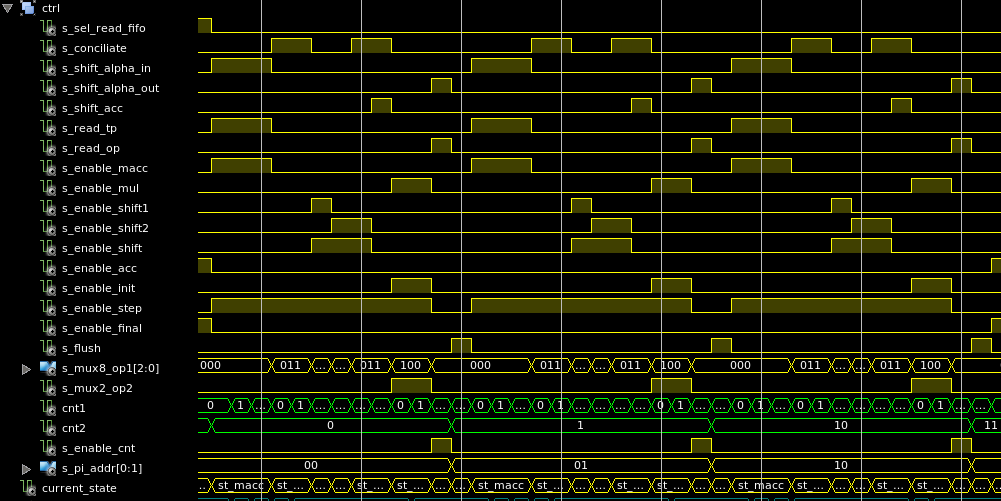
\includegraphics[width=1\columnwidth]{./schema/test_ctrl.png}
    \caption{Simulation example of the controller}
    \label{fig:test_ctrl}
\end{figure}

The implementation as been kept as generic as possible with only
one configuration package that allows to set the values $N$, $L$ and $M$ as well
as the operand widths. This generic options have however no impact on the
blocks automatically generated by the Xilinx CORE Generator
tool\footnote{http://www.xilinx.com/tools/coregen.htm}. These need to be
generated again if parameters in the configuration package are changed.

A big issue going from simulation to a real implementation on a physical
\gls{hw} board, are the timing constraints. In order to operate at a specific
frequency, the longest critical path is not allowed to be longer than the
period.  Synthesizer options like "register balancing" may help to reduce the
critical path, but often there is no way around adding additional registers
(and increase the pipeline length and hence the latency) or manually placing
critical components in closer proximity to each other. Optimizations for higher
frequencies have not been done. The goal was to run the accelerator at 100MHz.

%===============================================================================
%%%%%%%%%%%%%%%%%%%%%%%%%%%%%%%%%%%%%%%%%%%%%%%%%%%%%%%%%%%%%%%%%%%%%%%%%%%%%%%%
\chapter{Results}
\label{ch:results}
\glsresetall % reset acronyms

\begin{itemize}
    \item nexys4 board with artix-7 fpga
    \item limited recourses -> proof of concept
    \item bord \gls{hw} for testing
\end{itemize}

%-------------------------------------------------------------------------------
%===============================================================================
\section{Speedup}

%-------------------------------------------------------------------------------
%===============================================================================
\section{Accuracy}

%===============================================================================
%%%%%%%%%%%%%%%%%%%%%%%%%%%%%%%%%%%%%%%%%%%%%%%%%%%%%%%%%%%%%%%%%%%%%%%%%%%%%%%%
\chapter{Conclusion}
\label{ch:conc}
\glsresetall % reset acronyms

%-------------------------------------------------------------------------------
%===============================================================================
\section{Main Contribution}
\label{ch:conc_ach}

This thesis proposes a novel design of the basic forward algorithm on
\gls{fpga}, by using a fixed point representation and a custom operand scaling
scheme. The pipelined architecture allows to reduce memory access by a factor
of $L$. As the design targets embedded systems, the main focus was to reduce
the resource footprint as much as possible while keeping throughput and latency
at an acceptable level.

The thesis further proposes a design solution for a failure prediction model,
described in \cite{salfner08}. This includes the design of an extension to the
forward algorithm, a classifier and a memory management. The extension is
designed by adding a computation unit to calculate a new transition
probability matrix for every arriving observation symbol (the delay of one
symbol with respect to another is taken into account). The proposed design
of the predictor allows to implement a system capable of predicting one failure
type on a \gls{fpga} board, by using custom peripherals (\gls{ram}, Flash,
communication interface).

On a conceptional point of view, the thesis provides argumentation on why
in a world full of cloud server systems a failure prediction system for a single
node can still be beneficial.

%-------------------------------------------------------------------------------
%===============================================================================
\section{Future Work}
\label{ch:conc_work}

\begin{itemize}
    \item sparse matrix storage implementation
    \item study of parallelism options for sparse matrices
    \item thorough study of floating point implementation on \gls{fpga}
    \item implementation of the extension
    \item fixed-point design and implementation of the extension
    \item real case application implementation with proper memory interface
\end{itemize}

\nocite{*}

\appendix %optional, use only if you have an appendix

%===============================================================================
%%%%%%%%%%%%%%%%%%%%%%%%%%%%%%%%%%%%%%%%%%%%%%%%%%%%%%%%%%%%%%%%%%%%%%%%%%%%%%%%
\chapter{some material}
%\section{it's over\dots}

\backmatter

%\chapter{glossary} %optional

%\bibliographystyle{alpha}
%\bibliographystyle{dcu}
%\bibliographystyle{plainnat}
%\bibliographystyle{plain}
%\bibliographystyle{abbrvnat}
\bibliographystyle{siam}
%\bibliographystyle{ieeetr}
\bibliography{biblio}
\printglossaries

%\cleardoublepage
%\theindex %optional, use only if you have an index, must use
	  %\makeindex in the preamble

\end{document}
